%LTeX: language=pt-br
\documentclass[12pt,a4paper,oneside]{article}



%%%%%%%%%%%%%%%%%%%%%%%%%%%%%% Pacotes: basicos %%%%%%%%%%%%%%%%%%%%%%%%%%%%%% 
\usepackage[utf8]{inputenc}
\usepackage[T1]{fontenc}
\usepackage[brazil]{babel}
\usepackage[sectionbib]{natbib}

\usepackage{chapterbib}  

\usepackage{cmap}
\usepackage[margin=1cm,top=1cm,bottom=1cm,outer=1.5cm,includefoot]{geometry}
\usepackage{helvet}
\renewcommand{\familydefault}{\sfdefault}

\counterwithin*{equation}{section}
\counterwithin*{figure}{section}

\usepackage{titlesec}


%\usepackage[nottoc,numbib]{tocbibind}



\usepackage{fancyhdr}
\pagestyle{fancyplain}
\fancyhf{}
\lfoot{ \fancyplain{}{\footnotesize  IM381 - Elementos Finitos I} }
\rfoot{ \fancyplain{}{\footnotesize  \thepage} }
\renewcommand{\headrulewidth}{0pt}
\renewcommand{\footrulewidth}{1pt}

\usepackage{indentfirst}
\usepackage{enumerate}

%%%%%%%%%%%%%%%%%%%%%%%%%%%%%%% Fonte %%%%%%%%%%%%%%%%%%%%%%%%%%%%%%%%%%%%%%%%%%%%%%

\makeatletter
\renewcommand\footnotesize{\@setfontsize\footnotesize{9pt}{11}}
\makeatother

\makeatletter
\renewcommand\small{\@setfontsize\small{10pt}{12}}
\makeatother

\makeatletter
\renewcommand\normalsize{\@setfontsize\normalsize{12pt}{13}}
\makeatother

\makeatletter
\renewcommand\large{\@setfontsize\large{14pt}{14}}
\makeatother

\makeatletter
\renewcommand\Large{\@setfontsize\Large{16pt}{16}}
\makeatother


%%%%%%%%%%%%%%%%%%%%%%%%%%%%%%% Pacotes: links %%%%%%%%%%%%%%%%%%%%%%%%%%%%%%%

\usepackage[hidelinks]{hyperref}


%%%%%%%%%%%%%%%%%%%%%%%%%%%%%%%% Pacotes: ams %%%%%%%%%%%%%%%%%%%%%%%%%%%%%%%% 


\usepackage{amsmath}
\usepackage{amssymb}
\usepackage{tabularx}
\usepackage{scalerel}
\usepackage{listings}
\usepackage{bm}

%%%%%%%%%%%%%%%%%%%%%%%%%%%%%% Pacotes: figuras %%%%%%%%%%%%%%%%%%%%%%%%%%%%%% 
\usepackage{graphicx}
\usepackage{float}
\usepackage[table,xcdraw]{xcolor}

\usepackage{caption}
\usepackage{subcaption}

\usepackage{setspace}
\singlespacing

\usepackage{helvet}

\hypersetup{
    colorlinks=true,
    linkcolor=black,
    filecolor=black,      
    urlcolor=blue,
	citecolor=black,
}


\usepackage{listings}
\usepackage{color}

\definecolor{dkgreen}{rgb}{0,0.6,0}
\definecolor{gray}{rgb}{0.5,0.5,0.5}
\definecolor{mauve}{rgb}{0.58,0,0.82}
\definecolor{dkorange}{rgb}{0.97,0.45,0.25}

\lstset{frame=tb,
  language=Python,
  aboveskip=3mm,
  belowskip=3mm,
  showstringspaces=false,
  columns=flexible,
  basicstyle={\small\ttfamily},
  numbers=none,
  numberstyle=\tiny\color{gray},
  keywordstyle=\color{mauve},
  commentstyle=\color{gray},
  stringstyle=\color{dkgreen},
  breaklines=true,
  breakatwhitespace=true,
  tabsize=3,
  classoffset=1,        
  keywordstyle=\color{dkorange},
  classoffset=0,          
}

\DeclareMathOperator*{\assembly}{\scalerel*{\mathsf{A}}{\sum}}

\newcommand{\sing}[3]{{\left\langle #1-#2\right\rangle^{#3}}}
\usepackage{amsmath,scalefnt}
\usepackage{afterpage} 

\newcommand\blankpage{%
    \null
    \thispagestyle{empty}%
    \addtocounter{page}{-1}%
    \newpage}
 
\begin{document}

	

\newcommand{\HRule}{\rule{\linewidth}{0.5mm}} % Defines a new command for the horizontal lines, change thickness here

\vspace*{6cm}
\begin{center}

\HRule \\[0.4cm]
{ \huge \bfseries IM381 - Elementos Finitos I}\\[0.4cm] % Title of your document
\HRule \\[1.0cm]

\vspace*{2cm}

Professor: Heitor Nigro Lopes


\vspace*{12cm}

\today

\end{center}
	\thispagestyle{empty}
	\cleardoublepage

	\tableofcontents
	\cleardoublepage


	%LTeX: language=pt-br
% !TeX root = Apostila_IM381.tex

\section{Introdução}

    \subsection{Sobre a apostila e o método}

        Esta apostila serve como base para a disciplina IM381 - Elementos Finitos I, do programa de Engenharia Mecânica da Faculdade de Engenharia Mecânica da Universidade Estadual de Campinas. Esta apostila tem como objetivo auxiliar os alunos desta disciplina o acompanhamento destes no curso. Ela não tem pretensão de substituir qualquer livro, e um aprendizado adequado aos conteúdos apresentados aqui deve ser feito com auxílio de um bom livro de Elementos Finitos da literatura. 

        Esta apostila se encontra em um estágio inicial ainda, vários erros ainda podem estar presentes nela, entretanto, sugere-se cautela dos alunos estudando com base nela. Em caso de dúvidas, ou caso você deseje reportar algum erro ou fazer alguma sugestão, entre em contato com o autor por \url{hnlopes@unicamp.br}.

    \subsection{Instalação da biblioteca}

        Esta disciplina, quando ministrada pelo autor desta apostila, conta com o auxílio da biblioteca em Python de elementos finitos desenvolvido por seu grupo de pesquisa. Esta biblioteca se chama finelpy (Finite Element Python library). O código base desta biblioteca pode ser encontrado em \url{https://github.com/Lopes941/finelpy}, sendo esta programada nas linguagens Python e C++.

        A instalação dessa biblioteca pode ser feita pelo Python Package Index (PyPI). 

        \begin{center}
            \fbox{pip install finelpy}
        \end{center}

        
        Segue uma breve indicação de como começar a usar o Python em um computador com Windows.

        \subsubsection*{Instalação do Anaconda}

        Anaconda é uma plataforma para distribuição e para rodar programas em linguagem Python. Para alguém que nunca usou essa linguagem, talvez seja a plataforma mais intuitiva para iniciar. A instalação é feita diretamente no site em \url{https://www.anaconda.com/download/success}. Sinta-se livre para baixar a versão completa ou o miniconda.

        Ao instalar, abra o navegador conda (Anaconda Navigator). Na aba ``Home'', haverá vários softwares e IDEs que você pode usar. Aqui, usaremos o Spyder, por se tratar do mais parecido com o MATLAB, com o qual alguns alunos talvez já tenham familiaridade. A página principal do Spyder é conforme a Figura \ref{fig:spyder}.

        \begin{figure}[h!]
            \centering
            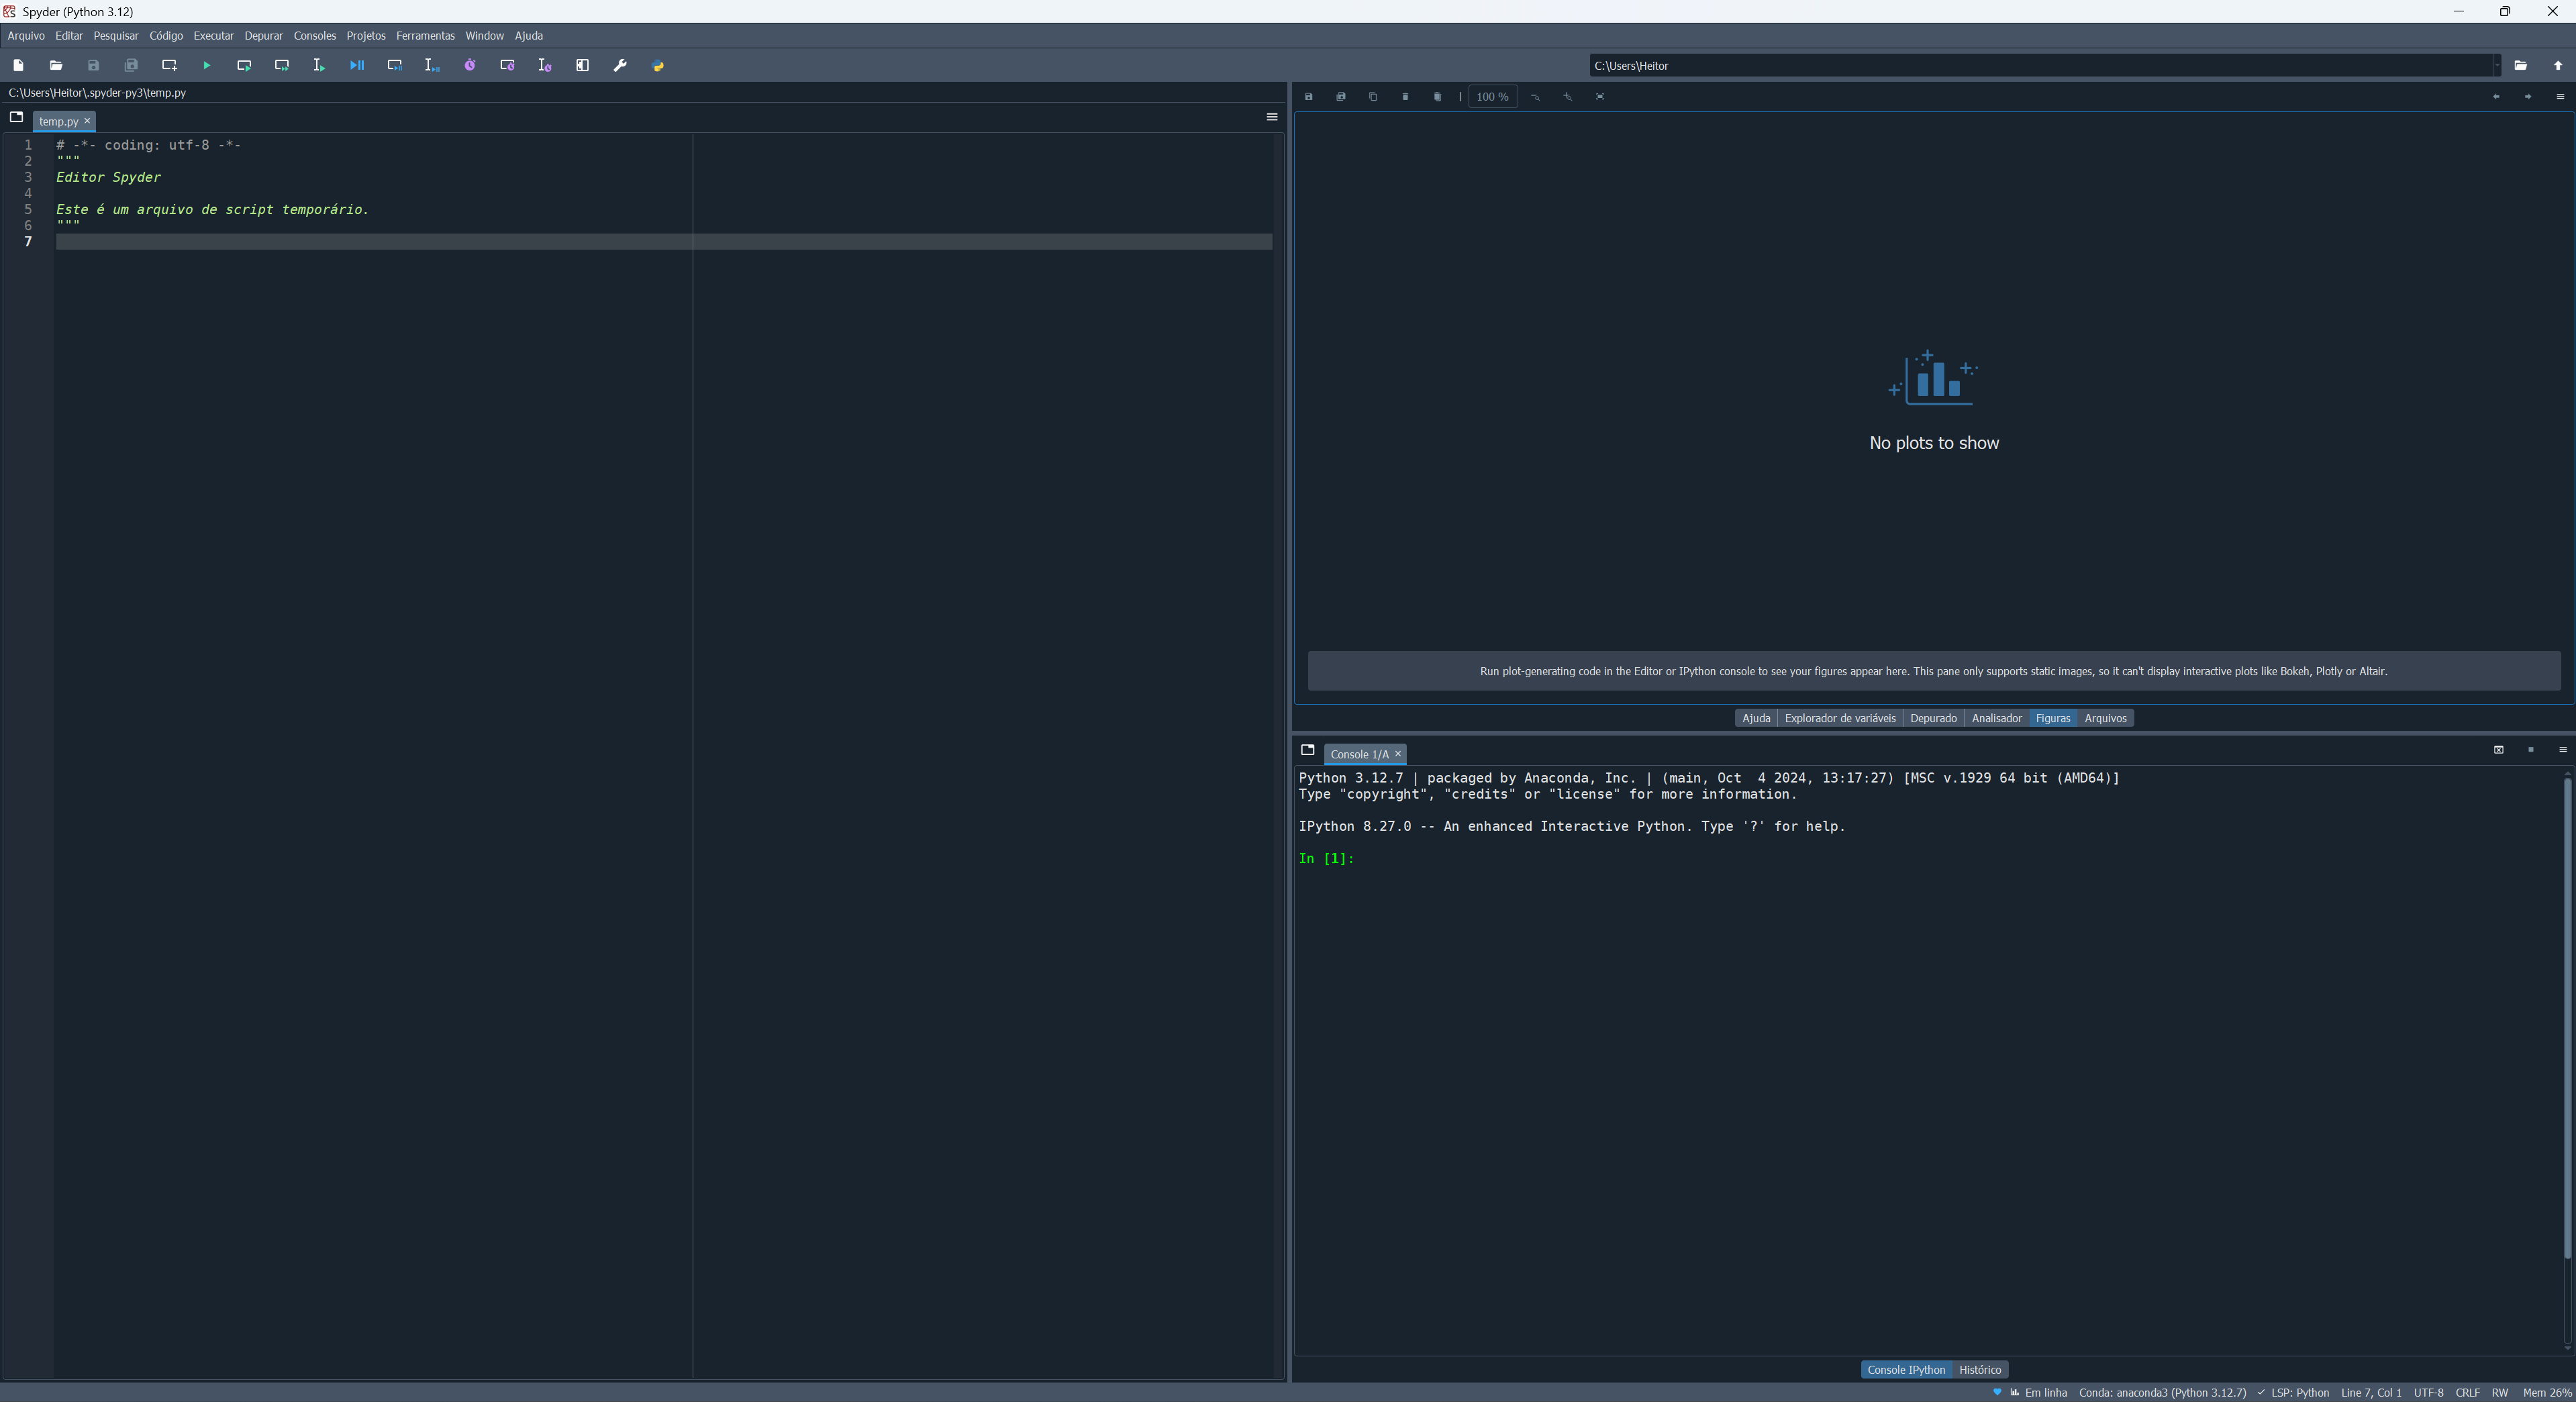
\includegraphics[scale=0.25]{Figures/1-Introducao/Spyder.png}
            \caption{Interface do Spyder ao abri-lo a primeira vez}
            \label{fig:spyder}
        \end{figure}




        Uma recomendação, caso você deseje que as figuras abram em outra janela, é abrir ``Preferências'' (O ícone de chave de boca), ``Console IPython'', ``Plotting'' e mudar ``Saída'' de ``Em linha'' para ``Automático''.
        

        
    \subsection{Revisão programação em Python}

        O Python é uma linguagem de programação bastante simples. Um programa simples para rodar ``Hello World'' é dado da simples forma:

        \begin{lstlisting}[language=Python]
            print("Hello world")
        \end{lstlisting}


        No Python, a indentação (o espaçamento antes de iniciar o texto em cada linha) é fundamental. Este espaçamento indica a hierarquia das estruturas de programação. Ele que indica onde um \textit{if}, \textit{for}, \textit{while}, ou função começa e termina. Por exemplo, o programa a seguir utiliza um \textit{if} para imprimir se um número é par ou ímpar:

        \begin{lstlisting}[language=Python]
            # Em Python, o simbolo # indica um comentario
            N = 3 #Numero inteiro que sera avaliado 
            
            # O simbolo % retorna o resto da divisao
            if N % 2 == 0:
                print(f"O numero {N} e par")
            else:
                print(f"O numero {N} e impar")
        \end{lstlisting}

        Perceba que após o \textit{if}, há um espaçamento com Tab, indicando o que está no \textit{if}. Mesma coisa para o \textit{else}.

        O \textit{for} percorre alguma lista ou vetor. A forma mais tradicional de percorrer um \textit{for} em Python é utilizando o \textit{range}. Observe o programa abaixo que calcula o quadrado de alguns números.

        \begin{lstlisting}[language=Python]
            # Exemplo 1 - calculando o quadrado de 0 a 3
            for i in range(4):
                # Em Python, o operador ^ se faz com **
                print(i**2)

            # >> 0
            # >> 1
            # >> 4
            # >> 9

            # Exemplo 2 - calculando o quadrado de 2 a 3
            for i in range(2,4):
                print(i**2)

            # >> 4
            # >> 9

            # Podemos percorrer diretamente os itens de uma lista
            # Exemplo 3 - calculando o quadrado dos itens de uma lista
            lista = [4, 2, 5]
            for i in lista:
                print(i**2)

            # >> 16
            # >> 4
            # >> 25

            # Uma estrutura Python bem comum tambem se trata do enumerate
            # enumerate retorna o indice do elemento na lista e o valor
            # deste elemento
            # Exemplo 4 - mesmo caso, com enumerate

            lista = [4, 2, 5]
            for i,item in enumerate(lista):
                valor = item**2
                print(f"O quadrado do {i}-esimo elemento e: {valor}")

            # >> O quadrado do 0-esimo elemento e: 16
            # >> O quadrado do 1-esimo elemento e: 4
            # >> O quadrado do 2-esimo elemento e: 25

        \end{lstlisting}


        Outra funcionalidade importante é a definição de funções. Podemos definir uma função com a palavra chave ``def'', em algum lugar do nosso código. Por exemplo, observe o programa abaixo que retorna um número elevado ao outro.

        \begin{lstlisting}[language=Python]
            
            # Funcao que retorna a elevado a b
            def quadrado(a,b):
                return a**b

            # Para rodar a funcao, apenas chamamos ela
            valor1 = quadrado(2,4)
            valor2 = quadrado(5,2)

            print(valor1, valor2)
            # >> 16
            # >> 25

        \end{lstlisting}

        Por último, outra funcionalidade que utilizaremos é a definição de classes. Uma classe é um objeto que carrega consigo algumas funções próprias e variáveis. Nas funções da classe, aparece a variável \textit{self}, que se refere ao próprio objeto. Toda classe tem uma função \_\_\textit{init}\_\_(), que é rodada ao criar uma variável do tipo desta classe.
        
        Por exemplo:

        \begin{lstlisting}[language=Python]
            
            # Classe pessoa, que carrega a idade e o nome.
            
            class Pessoa:

                # Construtor da classe
                def __init__(self, nome, idade):
                    self.nome = nome
                    self.idade = idade

                # Funcao que retorna se aquela pessoa 
                # tem idade para votar
                def pode_votar(self):
                    return self.idade >= 16

            lucas = Pessoa("Lucas",15)
            maria = Pessoa("Maria",40)
            
            print(lucas.pode_votar())
            print(lucas.idade)
            print(maria.pode_votar())
            print(maria.nome)

            # >> False
            # >> 15
            # >> True
            # >> "Maria"

        \end{lstlisting}

        Uma funcionalidade importante de classes é a herança. É possível criar uma classe que herde funções de uma classe pai:

        \begin{lstlisting}[language=Python]
            
            # Classe pessoa, que carrega a idade e o nome.

            class Pessoa:
                def __init__(self, nome, idade):
                    self.nome = nome
                    self.idade = idade

                def pode_votar(self):
                    return self.idade >= 16
            
            class Estudante(Pessoa):

                def __init__(self, nome, idade, curso):
                    #Roda o __init__ da classe pai
                    super().__init__(nome,idade) 
                    self.curso = curso
                
                def nome_do_curso():
                    return self.curso

            leo = Estudante("Leonardo",19,"Engenharia Mecanica")
            maria = Pessoa("Maria",40)
            
            print(leo.pode_votar())
            print(leo.nome_do_curso())
            print(maria.pode_votar())

            # print(maria.nome_do_curso())
            # Nao roda, pois maria e uma Pessoa
            # mas nao e Estudante

            # >> True
            # >> "Engenharia Mecanica"
            # >> True

        \end{lstlisting}
        
        \subsubsection*{Biblioteca Numpy}

        No Python, é usual utilizar bibliotecas que possuem já possuem funções prontas. A biblioteca mais comum para manipulações matemáticas é o Numpy. O Numpy é usado para manipulação de vetores de matrizes, assim como para utilizar funções matemáticas mais comuns. O exemplo abaixo mostra como importar o numpy (usualmente importado sob o nome ``np''), usá-lo para criar um vetor com N pontos linearmente espaçados e calcular o seno desses pontos:

        \begin{lstlisting}
            # Importa biblioteca numpy
            import numpy as np

            # Cria um vetor com 11 pontos linearmente espacados
            # entre 0 e 1, incluindo 0 e 1.
            v = np.linspace(0,1,11)
            print(v)

            # >> [0, 0.1, 0.2, 0.3, 0.4, 0.5, 0.6, 0.7, 0.8, 0.9, 1.0]

            # Calcula o seno dos pontos (v em radianos)
            sen_v = np.sin(v)
            print(sen_v)

            # >>[0.         0.09983342 0.19866933 0.29552021 0.38941834 
            # >> 0.47942554 0.56464247 0.64421769 0.71735609 0.78332691 
            # >> 0.84147098]

        \end{lstlisting}

        Recomenda-se fazer manipulações matemáticas diretamente em um vetor numpy do que fazer termo a termo. Como o Python é uma linguagem interpretada, e o numpy possui funções pré-compiladas, manipular os vetores diretamente é muito mais rápido:

        \begin{lstlisting}
            import numpy as np

            v = np.linspace(0,1,11)

            # Opcao 1 - Lento
            sen_v = np.empty(11) # Cria um vetor tamanho 11 "vazio"
            for i,vi in enumerate(v):
                sen_v[i] = np.sin(vi)

            # Opcao 2 - Mais rapido (recomendado)
            sen_v = np.sin(v)

        \end{lstlisting}

    \subsection{Revisão de conceitos de cálculo}

        Na definição do Método de Elementos Finitos, são necessários alguns conceitos de cálculo. Nesta seção, será apresentado alguns conceitos de cálculo importantes.

        \subsubsection*{Derivada de uma função}

        Seja uma função $f(x)$, sua derivada em um ponto $x=a$ é definida pelo limite:

        \begin{equation*}
            \left.\frac{df}{dx}\right|_{x=a} = f'(a) = \lim_{\Delta x\rightarrow 0 }\frac{f(a+\Delta x)-f(a)}{\Delta x}
        \end{equation*}

        De forma geral, podemos escrever uma função $\frac{df}{dx}$ das derivadas de $f(x)$ em um dado intervalo $\Omega$. As funções mais comuns e suas derivadas são:

        \begin{equation*}
            f(x) = x^n \rightarrow f'(x) = n x^{n-1}
        \end{equation*}

        \begin{equation*}
            f(x) = sen(x) \rightarrow f'(x) = cos(x)
        \end{equation*}

        \begin{equation*}
            f(x) = cos(x) \rightarrow f'(x) = -sen(x)
        \end{equation*}

        E algumas relações importantes são: a \textbf{regra do produto}:

        \begin{equation*}
            \frac{d}{dx}\left(f(x) \cdot h(x)\right) = \frac{df(x)}{dx} \cdot h(x) + f(x) \cdot \frac{dh(x)}{dx},
        \end{equation*}

        \noindent a \textbf{regra do quociente}:

        \begin{equation*}
            \frac{d}{dx}\left(\frac{f(x)}{ h(x)}\right) = \frac{\frac{df(x)}{dx} \cdot h(x) - f(x) \cdot \frac{dh(x)}{dx}}{h(x)^2},
        \end{equation*}

        \noindent e a \textbf{regra da cadeia}:

        \begin{equation*}
            \frac{d}{dx}\left[f(h(x))\right] = \frac{df}{dh} \cdot \frac{dh}{dx},
        \end{equation*}

        A derivada da função derivada é a \textbf{derivada segunda}, e assim sucessivamente:

        \begin{equation*}
            f''(x) = \frac{d^2f}{dx^2} = \frac{df'}{dx}
        \end{equation*}

        \begin{equation*}
            \frac{d^nf}{dx^n} = \frac{d}{dx} \left(\frac{d^{n-1}f}{dx^{n-1}}\right)
        \end{equation*}

        Para funções com mais de uma variável, como $f(x,y,z)$, podemos definir derivadas em relação a cada variável, neste caso, temos uma \textbf{derivada parcial}:

        \begin{equation*}
            \frac{\partial f}{\partial x}, \quad \frac{\partial f}{\partial y}, \quad \frac{\partial f}{\partial z}
        \end{equation*}

        O \textbf{gradiente} de uma função de mais de uma variável é um vetor tal que cada componente é uma derivada parcial:

        \begin{equation*}
            grad \; f = \nabla f = 
            \begin{Bmatrix}
                \frac{\partial f}{\partial x}\\
                \frac{\partial f}{\partial y}\\
                \frac{\partial f}{\partial z}
            \end{Bmatrix}
        \end{equation*}

        Uma \textbf{função vetorial}, é um vetor que cada termo é uma função, por exemplo:

        \begin{equation*}
            \mathbf{f}(x,y) = 
            \begin{Bmatrix}
                f_1(x,y)\\
                f_2(x,y)
            \end{Bmatrix}
        \end{equation*}

        O \textbf{divergente} de uma função vetorial é a soma das derivadas em relação a cada variável:

        \begin{equation*}
            div \; \mathbf{f} = 
            \nabla \cdot \mathbf{f} = 
            \frac{\partial f_1}{\partial x} + \frac{\partial f_2}{\partial y}
        \end{equation*}

        O gradiente de uma função vetorial é uma matriz em que cada linha é o gradiente de cada função

        \begin{equation*}
            grad \; \mathbf{f} = 
            \nabla \mathbf{f} = 
            \begin{bmatrix}
                \frac{\partial f_1}{\partial x} & \frac{\partial f_2}{\partial x} \\
                \frac{\partial f_1}{\partial y} & \frac{\partial f_2}{\partial y}
            \end{bmatrix}
        \end{equation*}

        O \textbf{laplaciano} é o divergente do gradiente de uma função escalar:

        \begin{equation*}
            \Delta f(x) = \nabla \cdot \left(\nabla f(x)\right) = \nabla \cdot 
            \begin{Bmatrix}
                \frac{\partial f}{\partial x}\\
                \frac{\partial f}{\partial y}
            \end{Bmatrix} =
            \frac{\partial^2 f_1}{\partial x^2} + \frac{\partial^2 f_2}{\partial y^2}
        \end{equation*}


        \subsubsection*{Integral de uma função}

        Nesta disciplina, usaremos integrais definidas. Uma integral definida (integral de Riemann) em um intervalo $\Omega = (a,b)$ é definida como:
        
        \begin{equation*}
            \int_{a}^{b} f(x) dx = \lim_{i\rightarrow\infty} \sum_{i=1}^n f(x_i) \Delta x_i, \quad \Delta x_i = \frac{b-a}{n}
        \end{equation*}

        Segundo o teorema fundamental do cálculo, uma integral pode ser vista como a operação inversa da derivada:

        \begin{equation}
            \int_{a}^{b} f'(x) dx = f(b)-f(a)
        \end{equation}

        Portanto, para integrar uma função, normalmente utilizam-se procedimentos para facilitar encontrar a função cuja derivada é o integrando. 
        
        Um procedimento é o da \textbf{substituição de variáveis}. Dada a integral:

        \begin{equation*}
            \int_{x_1}^{x_2} f(x) dx
        \end{equation*}
        
        \noindent se conseguirmos definir uma variável $y$, com $x(y)$, tal que $dx = \frac{dx}{dy} dy$, $x_1 = x(y_1)$ e $x_2 = x(y_2)$. Então podemos reescrever a integral como:

        \begin{equation*}
            \int_{x_1}^{x_2} f(x) dx = 
            \int_{y_1}^{y_2} f(x(y)) \frac{dx}{dy} dy
        \end{equation*}
        
        Outro procedimento usual é a \textbf{integração por partes:}

        \begin{equation}
            \int_{a}^{b} f'(x) h(x) dx = \left[f(x)h(x)\right]_{a}^{b} - \int_{a}^{b} f(x) h'(x) dx
        \end{equation}


        Uma integral dupla, tripla, e assim sucessivamente, é uma integral definida de funções de mais de uma variável:

        \begin{equation*}
            \int_{y_1}^{y_2} \int_{x_1}^{x_2} f(x,y) dx dy
        \end{equation*}

        Em uma área qualquer $\Omega$, vamos escrever como:

        \begin{equation*}
            \int_{\Omega} f(x,y) dA
        \end{equation*}

        Considerando uma área $\Omega$ definida pelo sistema de coordenadas $xy$, podemos realizar uma mudança de coordenadas na integração para a mesma área, porém descrita por um sistema de coordenadas diferente $\hat{x}\hat{y}$, da seguinte forma:

        \begin{equation*}
            \int_{\Omega} f(x,y) dA = \int_{\Omega} f(x(\hat{x},\hat{y}),y(\hat{x},\hat{y})) \det \mathbf{J} d\hat{A}
        \end{equation*}

        \noindent no qual:

        \begin{equation*}
            \mathbf{J} = 
            \begin{bmatrix}
                \frac{\partial x}{\partial \hat{x}} & \frac{\partial y}{\partial \hat{x}}\\
                \frac{\partial x}{\partial \hat{y}} & \frac{\partial y}{\partial \hat{y}}
            \end{bmatrix}
        \end{equation*}

        Dada uma superfície $\Gamma$ no espaço $\mathbb{R}^3$, uma \textbf{integral de superfície} é dada por:

        \begin{equation*}
            \int_{\Gamma} f dS
        \end{equation*}

        O \textbf{teorema do divergente} transforma a integral no volume do divergente de uma função vetorial em uma integral de superfície, ao longo da superfície do domínio de integração original:

        \begin{equation*}
            \int_{\Omega} \nabla \cdot \mathbf{f} dV = \int_{\partial \Omega}  \mathbf{f} \cdot \mathbf{n} dS
        \end{equation*}

        \noindent no qual $\partial \Omega$ é o fecho de $\Omega$, isto é, o contorno fechado de $\Omega$, e $\mathbf{n}$ é o vetor normal à superfície, apontando para fora.

    \subsection{Revisão de conceitos de álgebra linear}
    \label{sec:algelin}

        A álgebra linear, embora não estritamente necessária para ter um entendimento básico e para aplicar o Método dos Elementos Finitos, é essencial para entender mais a fundo como este funciona. Portanto, esta seção apresenta a revisão de alguns conceitos básicos de espaço vetorial, e apresenta alguns espaços citados no texto.

        Um corpo $K$ é um conjunto no qual as operações de adição e multiplicação entre termos são definidas e satisfazem as seguintes condições:

        Axiomas da adição:
        \begin{itemize}
            \item \textit{Associatividade:} $(a+b)+c = a+(b+c)$
            \item \textit{Comutatividade:} $a+b=b+a$
            \item \textit{Elemento neutro:} $\exists 0 \in K : a+0=a, \forall a \in K$
            \item \textit{Simétrico:} $\forall a \in K, \exists (-a)\in K : a + (-a) = 0$
        \end{itemize}

        Axiomas da multiplicação:
        \begin{itemize}
            \item \textit{Associatividade:} $(a \cdot b) \cdot c = a \cdot (b \cdot c)$
            \item \textit{Comutatividade:} $a \cdot b=b \cdot a$
            \item \textit{Elemento neutro:} $\exists 1 \in K, 1\neq 0 : a \cdot 0 = 0, \forall a \in K$
            \item \textit{Inverso multiplicativo:} $\forall a \neq 0 \in K : \exists a^{-1}\in K : a \cdot a^{-1} = 1$
        \end{itemize}

        Um corpo ordenado é aquele no qual os seus elementos podem ser descritos como positivos, negativos ou zero. O conjunto dos números reais $\mathbb{R}$ é um corpo ordenado completo.

        Um espaço vetorial $V$ sobre um corpo $K$ é um conjunto munido das operações de soma entre dois elementos de $V$ e de multiplicação por escalar, entre um elemento de $K$ e um elemento de $V$. Estas operações devem obedecem aos seguintes axiomas:

        \begin{itemize}
            \item \textit{Associatividade da adição:} $(\mathbf{u} + \mathbf{v}) + \mathbf{w} = \mathbf{u} + (\mathbf{v} + \mathbf{w})$
            \item \textit{Comutatividade da adição:} $\mathbf{u} + \mathbf{v} = \mathbf{v} + \mathbf{u}$
            \item \textit{Elemento neutro na adição:} $\exists \mathbf{0} \in V :\mathbf{u} + \mathbf{0} = \mathbf{u}$
            \item \textit{Simétrico na adição:} $\forall \mathbf{u} \in V, \exists (\mathbf{-u}) \in V :\mathbf{u} + (\mathbf{-u}) = \mathbf{0}$
            \item \textit{Associatividade na multiplicação por escalar:} $a,b \in K, u \in V : a(b\mathbf{u}) = (ab)\mathbf{u}$
            \item \textit{Elemento neutro na multiplicação por escalar:} seja $1$ o elemento neutro de $K : 1\mathbf{u} = \mathbf{u}$
            \item \textit{Distributividade do vetor na multiplicação por escalar:} $a(\mathbf{u} + \mathbf{v}) = a\mathbf{u} + a\mathbf{v}$
            \item \textit{Distributividade do escalar na multiplicação por escalar:} $(a+b)\mathbf{u} = a\mathbf{u} + b\mathbf{u}$
        \end{itemize}

        O espaço vetorial mais fácil de entender visualmente é o espaço vetorial dos vetores em $\mathbb{R}^3$, representado por ``setas'' no espaço tridimensional. Entretanto, essas definições podem ser aplicadas mesmo em conceitos mais amplos de espaço vetorial.

        A \textbf{dimensão} de um espaço vetorial é número de variáveis independentes (em $K$) necessárias e suficientes para representar, de forma única, um vetor em $V$. Por exemplo, o espaço $\mathbb{R}^3$ tem dimensão $3$, pois precisamos de três números independentes para representar um vetor, por exemplo, suas três componentes no sistema cartesiano.

        Uma \textbf{base} é um conjunto de vetores linearmente independentes que podem representar qualquer vetor do espaço vetorial. Um conjunto de vetores linearmente independentes de um espaço de dimensão $n$ ($\mathbf{u}_1, \mathbf{u}_2, \ldots, \mathbf{u}_n$) é aquele que nenhum vetor da base pode ser escrito como uma combinação linear dos outros, isto é, não existe nenhuma combinação de escalares ($a_1, a_2, \ldots, a_n$), tal que um vetor possa ser escrito como uma soma dos outros:

        \begin{equation}
            \mathbf{u}_j \neq a_1 \mathbf{u}_1 + \cdots + a_{j-1} \mathbf{u}_{j-1} + a_{j+1} \mathbf{u}_{j+1} + \cdots + a_n \mathbf{u}_n = \sum\limits_{\underset{i\neq j}{i=0}}^n a_i \mathbf{u}_i , \quad \forall a_1, a_2, \ldots, a_n \in K
        \end{equation}

        Qualquer vetor do espaço vetorial pode ser escrito de forma única como uma combinação linear dos vetores que formam uma base:

        \begin{equation}
            \mathbf{v} = a_1 \mathbf{u}_1 + \cdots + a_{i} \mathbf{u}_{i} + \cdots + a_n \mathbf{u}_n = \sum\limits_{i=0}^n a_i \mathbf{u}_i
        \end{equation}

        Por exemplo, para o espaço vetorial $\mathbb{R}^3$, normalmente é usada a base ortogonal dos vetores unitários $\mathbf{i}, \mathbf{j}, \mathbf{k}$, de forma que qualquer $\mathbf{u}$ pode ser escrito como:

        \begin{equation}
            \mathbf{u} = u_x \mathbf{i} + u_y \mathbf{j} + u_z \mathbf{k}
        \end{equation}

        O espaço vetorial dos polinômios de grau menor ou igual a $2$, denominado $\mathcal{P}_2$, tem dimensão $3$ e pode ser escrito pela base $p_1(x) = 1, p_2(x) = x, p_3(x) = x^2$, tal que, para qualquer polinômio deste espaço:

        \begin{equation}
            q(x) = a_0 + a_1x + a_2 x^2 = a_0 p_1(x) + a_1 p_2(x) + a_2 p_3(x)
        \end{equation}
    
        Existem espaços vetoriais de \textbf{dimensão infinita}, isso significa que não é possível escrever uma base para este espaço. Um exemplo de espaço vetorial de dimensão infinita é o espaço formado pelas funções suaves (funções contínuas com todas as derivadas contínuas) $\mathcal{C}^\infty$.

        Um \textbf{subespaço} é um espaço vetorial que é subconjunto de um espaço vetorial. Por exemplo, o espaço vetorial dos polinômios de grau menor ou igual 2 $\mathcal{P}_2$ é composta por funções suaves, portanto, $\mathcal{P}_2$ é um subespaço de $C^\infty$. Da mesma forma, polinômios de grau menor ou igual a 2 têm grau menor ou igual a 5, então $\mathcal{P}_2$ é um subespaço de $\mathcal{P}_5$. Note que subespaços sempre devem ter dimensão menor ou igual à dimensão do espaço maior.

        O \textbf{produto interno} é uma operação $\left\langle \cdot, \cdot \right\rangle $ entre dois vetores de um espaço vetorial que retornam um escalar. Ele deve obedecer às relações:

        \begin{itemize}
            \item \textit{Simetria conjugada:} $\left\langle \mathbf{u}, \mathbf{v} \right\rangle = \bar{\left\langle \mathbf{v}, \mathbf{u} \right\rangle}$
            \item \textit{Linearidade:} $\left\langle a\mathbf{u} + b\mathbf{v}, \mathbf{w} \right\rangle = \left\langle a\mathbf{u}, \mathbf{w} \right\rangle + \left\langle b\mathbf{v}, \mathbf{w} \right\rangle$
            \item \textit{Positividade:} $\left\langle \mathbf{u}, \mathbf{u} \right\rangle > 0 , \quad\forall \mathbf{u} \neq \mathbf{0}$
        \end{itemize}

        O exemplo mais usual de produto interno é o produto escalar entre vetores euclideanos:

        \begin{equation}
        \left\langle \mathbf{u}, \mathbf{v} \right\rangle  = 
        \mathbf{u} \cdot \mathbf{v} =
        \begin{Bmatrix}
            u_1\\
            u_2\\
            \vdots\\
            u_n
        \end{Bmatrix} \cdot
        \begin{Bmatrix}
            v_1\\
            v_2\\
            \vdots\\
            v_n
        \end{Bmatrix}
        =
        u_1 v_1 + u_2 v_2 + \cdots + u_n v_n
    \end{equation}

    Em espaços definidos por funções, o produto interno mais comum é dado por uma integral definida:

    \begin{equation}
        \left\langle p(x), q(x) \right\rangle  = \int_{a}^{b} p(x) \bar{q(x)} dx
    \end{equation}

    Dois vetores são ditos \textbf{ortogonais} se o produto interno entre eles for nulo. Desta forma, uma base ortogonal é formada por vetores linearmente independentes que também são ortogonais entre si.

    A definição de \textbf{norma} é baseada no produto interno e presenta uma operação do vetor sobre ele mesmo que retorna um escalar. Por exemplo, no espaço euclideano:

    \begin{equation}
        \left\Vert \mathbf{u} \right\Vert = \sqrt{\left\langle \mathbf{u},\mathbf{u} \right\rangle} = \sqrt{ u_1^2 + u_2^2 + \cdots + u_n^2}
    \end{equation}

    No caso de funções com o produto interno definido pela integral:

    \begin{equation}
        \left\Vert p(x) \right\Vert = \sqrt{\left\langle p(x),p(x) \right\rangle} = \int_{a}^{b} p(x)^2 dx
    \end{equation}

    \noindent como veremos logo a seguir, na próxima seção, o espaço vetorial munido dessa operação é chamado espaço de Lebesgue.

    \subsubsection*{Espaço de Sobolev}

    Com as definições anteriores, definiremos alguns espaços vetoriais de funções. O espaço $\mathcal{C}^p (\Omega)$ (às vezes representado apenas por $\mathcal{C}^p$) já citado anteriormente, é o espaço composto pelas contínuas em $\Omega$ e com até a $p$-ésima derivada também contínua em $\Omega$. Por exemplo, a função rampa:

        \begin{equation*}
            f(x) = \left\{\begin{array}{l}
                x, x \geq 0\\
                0, x<0
            \end{array}\right.,
        \end{equation*}

    é contínua, mas possui derivada não contínua no intervalo $\Omega = ]-\infty, \infty[$, portanto $f(x) \in \mathcal{C}^0(\Omega)$. Porém, no intervalo $\Omega_2 = [3, 10]$, por exemplo, ele possui derivadas contínuas não importa a ordem (a partir da segunda, se anula). Portanto, $f(x) \in \mathcal{C}^\infty(\Omega)$. O espaço $\mathcal{C}^\infty$ muitas vezes é chamado de espaço das \textbf{funções suaves}.


    Com as definições anteriores, podemos definir o \textbf{espaço de Lebesgue} $\mathcal{L}^p(\Omega)$. Este é composto pela funções $p$-integráveis, isto é:

        \begin{equation}
            \int_\Omega \left|f(x)\right|^p dx < \infty
        \end{equation}

    Normalmente, definem-se as funções quadrado integráveis $\mathcal{L}^2(\Omega)$:

    \begin{equation}
        \int_\Omega \left[f(x)\right]^2 dx < \infty
    \end{equation}

    A importância deste espaço, é que este define um espaço com um produto interno finito para todos os membros deste espaço, isto é:

    \begin{equation}
        \left\langle f(x), h(x) \right\rangle = \int_\Omega f(x)h(x) dx < \infty
    \end{equation}

    Finalmente, temos o \textbf{espaço de Sobolev} $\mathcal{H}^p(\Omega)$. Um espaço de Sobolev de ordem $p$ é aquele que todas as funções e todas as suas respectivas derivadas até a ordem $p$ pertencem a $\mathcal{L}^2(\Omega)$. Isto é:

    \begin{equation}
        \int_\Omega \left[f(x)\right]^2 dx < \infty
    \end{equation}

    \begin{equation}
        \int_\Omega \left[\frac{d^nf}{dx^n}\right]^2 dx < \infty \quad, \forall n \leq p
    \end{equation}

    A importância deste tipo de espaço está na solução de equações diferenciais. Considere a equação diferencial de ordem $n$ abaixo em algum domínio $\Omega$:

    \begin{equation*}
        p\left(x, f(x), \frac{df}{dx}, \ldots, \frac{d^nf}{dx^n}\right) + q(x) = 0,
    \end{equation*}

    \noindent então sabemos que, se existir solução, ela será um membro de $\mathcal{H}^p(\Omega)$.

    Esta relação será utilizada nos métodos para obter soluções aproximadas de equações diferenciais mostrados aqui. A solução da equação pertence ao espaço vetorial de dimensão infinita $\mathcal{H}^p(\Omega)$. A aproximação se baseará em encontrar a função em um subespaço de $\mathcal{H}^p(\Omega)$ de dimensão finita, por exemplo $\mathcal{P}_q$, que melhor se aproxima da solução real.

	%LTeX: language=pt-br
% !TeX root = Apostila_IM381.tex

\cleardoublepage
\section{Revisão modelo de barra}

    Nesta seção, será apresentada uma revisão do modelo de barra, sua equação diferencial, com alguns exemplos e exercícios.

    \subsection{Hipóteses}

        As principais hipóteses do modelo de barra são:

        \begin{itemize}
            \item Estrutura esbelta - comprimento muito maior que sua largura ou espessura;
            \item Material linear elástico isotrópico;
            \item Pequenas deformações e pequenos deslocamentos;
            \item Submetido apenas a cargas ao longo do seu comprimento;
            \item Deformações locais desprezíveis (princípio de Saint-Venant).
        \end{itemize}

        A última hipótese está relacionada ao princípio de Saint-Venant. Este afirma que, dado um conjunto de forças aplicada em uma parte da superfície de um corpo, tal que sua força e momento resultantes são nulos, então os efeitos de deformação devido a esta deve ser ínfima em regiões suficientemente distantes (Figura \ref{fig:venant}). Para a barra, isto implica em um perfil de forças uniforme.

        \begin{figure}[h!]
            \centering
            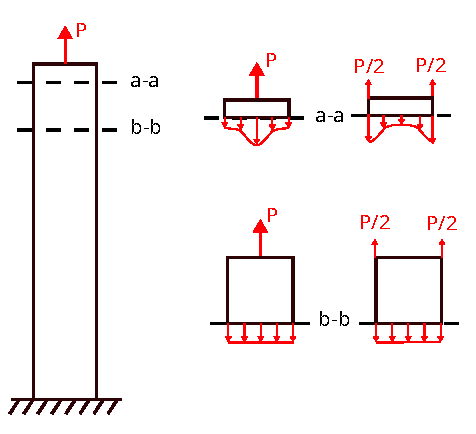
\includegraphics[scale=1]{Figures/2-Resmat/Venant.pdf}
            \caption{Princípio de Saint-Venant. Forças com mesma resultante possuem os mesmos efeitos se estivermos suficientemente distantes de seu ponto de aplicação.}
            \label{fig:venant}
        \end{figure}

    \subsection{Dedução da equação diferencial}

        Considere uma barra com uma área da seção transversal variável $A(x)$, sujeita a uma força distribuída $p(x)$. Fazendo de um elemento infinitesimal desta estrutura (Figura \ref{fig:barra}), podemos calcular o seu equilíbrio de forças:

        \begin{figure}[h!]
            \centering
            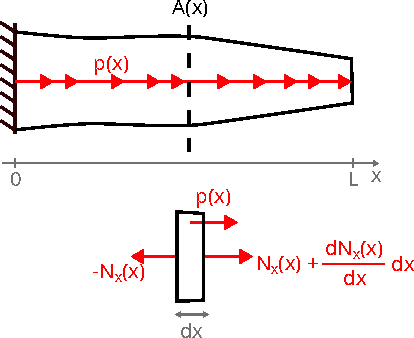
\includegraphics[scale=1]{Figures/2-Resmat/Bar.pdf}
            \caption{Equilíbrio de uma barra. Elemento infinitesimal da barra em equilíbrio.}
            \label{fig:barra}
        \end{figure}

        \begin{equation*}
            \sum F_x = 0
        \end{equation*}

        \begin{equation*}
            \frac{dN_x}{dx} = -p(x)
        \end{equation*}


        Conforme mencionado anteriormente, podemos considerar que os esforços internos ao longo da seção tranversal são uniformes. Portanto, a tensão normal $\sigma_{xx}$ é constante ao longo da largura e espessura:

        \begin{equation*}
            \int_A \sigma_{xx}(x) dA = N_x(x)
        \end{equation*}

        \begin{equation}
            \sigma_{xx}(x) = \frac{N_x(x)}{A(x)}
        \end{equation}


        Como o material é considerado linear elástico e isotrópico, podemos correlacionar as tensões com as deformações pela Lei de Hooke, a partir do Módulo de Young $E(x)$ do material:

        \begin{equation}
            \sigma_{xx}(x) = E(x)\varepsilon_{xx}(x)
        \end{equation}

        Finalmente, como os deslocamentos e as deformações são pequenas, os deslocamentos axiais $u(x)$ podem ser escritos como:

        \begin{equation}
            \frac{du(x)}{dx} = \varepsilon_{xx}(x)
        \end{equation}

        Juntando todas as expressões anteriores, chega-se à equação diferencial da barra:

        \begin{equation}
            \frac{d}{dx}\left(E A \frac{du}{dx}\right) = -p(x)
        \end{equation}

        Se considerarmos uma barra com seção transversal e módulo de elasticidade uniformes, chegamos à expressão simplificada:

        \begin{equation}
            E A \frac{d^2u}{dx^2} = -p(x)
        \end{equation}


        Esta equação deve ser resolvida com o auxílio de condições de contorno. Estas podem ser de dois principais tipos: condição de Dirichlet ou de Neumann. As condições de contorno de Dirichlet são condições no deslocamento na extremidade do domínio. Por exemplo, para uma barra de comprimento $L$ da Figura \ref{fig:barra_exemplo1}, com $x \in \left(0,L\right)$, podemos impor que $u(0) = u_0$. As condições de Neumann são condições na força aplicadas na extremidade do domínio. Por exemplo, para a mesma barra que a anterior, podemos aplicar uma força $F$ de tração na extremidade direita da barra. Neste caso, $N_x(L) = F$. Os sinais desta condição de contorno devem seguir o diagrama da Figura \ref{fig:convencao_normal}. Note que, embora usualmente estes diagramas sejam chamados de ``convenção da Resmat'', estes não são definidos arbitrariamente, mas são provenientes dos cálculos do equilíbrio.

        \begin{figure}[h!]
            \centering
            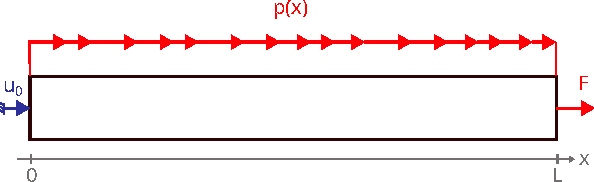
\includegraphics[scale=1]{Figures/2-Resmat/Barra_exemplo.pdf}
            \caption{Exemplo de barra com deslocamento imposto à esquerda e força aplicada à direita.}
            \label{fig:barra_exemplo1}
        \end{figure}

        \begin{figure}[h!]
            \centering
            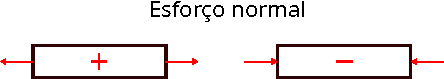
\includegraphics[scale=1]{Figures/2-Resmat/Esforcos.pdf}
            \caption{Convenção de sinais para esforços normais}
            \label{fig:convencao_normal}
        \end{figure}

        Desta forma, chega-se à seguinte equação diferencial para a barra (para este exemplo de condições de contorno):

        \begin{equation}
            \left\{
            \begin{array}{l}
                E A \frac{d^2u}{dx^2} = -p(x)\\
                u(0) = u_0\\
                N_x(L) = \left.EA\frac{du}{dx}\right|_{x=L} = F
            \end{array}
            \right.
        \end{equation}


    \subsection{Solução por funções de singularidade}
    \label{sec:singularidade}

        Para resolver a equação diferencial analiticamente, é necessário representar as forças como uma função $p(x)$. Entretanto, em muitos casos, a força não será contínua, como no caso de forças concentradas. Para representar essas forças, são usadas \textbf{funções de singularidade}.

        As funções de singularidade, de forma geral, são representadas por $\left\langle x-a \right\rangle^n$, modificando $a$ e $n$. Para representar uma força concentrada, podemos usar a função delta de Dirac. A função delta de Dirac é a função impulso unitário $\delta_a(x)$, conforme mostrado na Figura \ref{fig:dirac}, com o intervalo $\Delta$ sendo levado ao seu limite zero, tal que:

        \begin{figure}[h!]
            \centering
            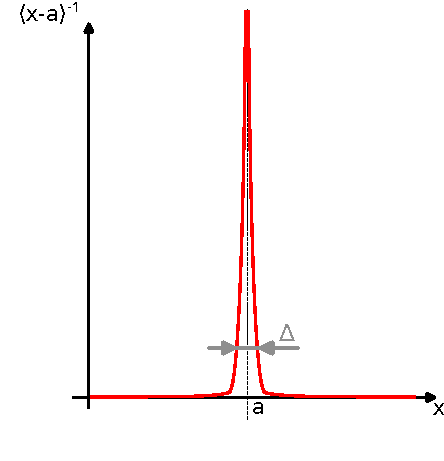
\includegraphics[scale=1]{Figures/2-Resmat/Dirac.pdf}
            \caption{Função impulso unitário.}
            \label{fig:dirac}
        \end{figure}

        \begin{equation*}
            \delta_a(x) = \left\{\begin{array}{l}
                0, x \neq a\\
                \text{não definido}, x=a
            \end{array}
            \right.
        \end{equation*}

        \begin{equation*}
            \int_{-\infty}^{\infty} \delta_a(x) dx = 1
        \end{equation*}

        No contexto de funções de singularidade, esta é $\delta_a(x) = \left\langle x-a\right\rangle^{-1}$

        Sua integral é a função degrau unitário (ou função Heaviside):

        \begin{equation*}
            H(x) = \left\langle x-a\right\rangle^0
            =
            \begin{array}{l}
                0, x < a\\
                1, x > a
            \end{array}
        \end{equation*}

        A partir de $n=0$, temos funções nulas para $x<a$ e polinomiais para $x\geq a$:

        \begin{equation*}
            \left\langle x-a\right\rangle^n =
            \left\{
            \begin{array}{l}
                0, x < a\\
                \left(x-a\right)^n, x > a
            \end{array}
            \right.
            \quad , n \in \left\{1,2, \ldots \right\}
        \end{equation*}

        A Figura \ref{fig:singularidade} ilustra algumas funções de singularidade.

        \begin{figure}[h!]
            \centering
            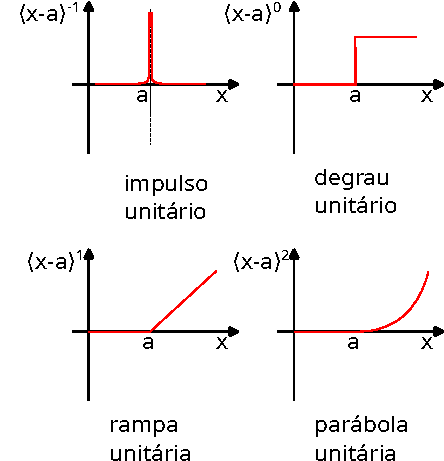
\includegraphics[scale=1.4]{Figures/2-Resmat/Singularidade.pdf}
            \caption{Funções de singularidade}
            \label{fig:singularidade}
        \end{figure}

        As derivadas das funções de singularidade podem, portanto, ser escrita da seguinte forma:

        \begin{equation*}
            \frac{d}{dx}\left\langle x-a\right\rangle^n =
            \left\{
            \begin{array}{l}
                \left\langle x-a\right\rangle^{n-1}, n \leq 0\\
                n\left\langle x-a\right\rangle^{n-1}, n > 0
            \end{array}
            \right.
        \end{equation*}

        As funções de singularidade podem ser usadas, portanto, para representar não apenas forças unitárias, mas também para forças distribuídas quaisquer no domínio. Na próxima seção, serão mostrados alguns exemplos de solução de problemas de barra por funções de singularidade.

    \subsection{Exemplos}

        \subsubsection{Exemplo 1:}

        Encontre o campo de deslocamento, os esforços internos e as reações de apoio da barra da Figura \ref{fig:barra_ex1}. Suponha $EA = 10^{3} N$.

        \begin{figure}[h!]
            \centering
            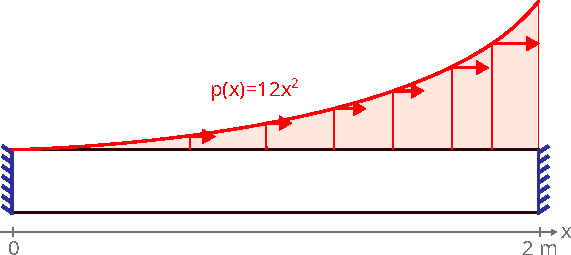
\includegraphics[scale=1]{Figures/2-Resmat/Exemplo1.pdf}
            \caption{Barra do Exemplo 1}
            \label{fig:barra_ex1}
        \end{figure}


        \subsubsection*{Solução:}

        O sistema está engastado nas duas extremidades, logo $u(0) = u(2) = 0$. A força distribuída pode ser escrita como:

        \begin{equation*}
            p(x) = 12x^2
        \end{equation*}

        Portanto, a equação diferencial é:

        \begin{equation*}
            \left\{
            \begin{array}{l}
                EAu''(x) = -12x^2\\
                u(0) = 0\\
                u(2) = 0
            \end{array}
            \right.
        \end{equation*}

        Para resolver, integramos sucessivamente a equação:

        \begin{equation*}
            EAu''(x) = -12x^2
        \end{equation*}

        \begin{equation*}
            EAu'(x) = -4x^3 + C_1
        \end{equation*}

        \begin{equation*}
            EAu(x) = -x^4 + C_1 x + C_2
        \end{equation*}

        \begin{equation*}
            u(x) = \frac{1}{EA} \left[-x^4 + C_1 x + C_2\right]
        \end{equation*}

        \noindent no qual as constantes $C_1$ e $C_2$ surgem da integração. Para obtê-las, aplicamos as condições de contorno:


        \begin{equation*}
            u(0) = 0 \rightarrow EAu(0) = -0^4 + C_1 0 + C_2 = 0
        \end{equation*}
        
        \begin{equation*}
            C_2 = 0
        \end{equation*}

        \begin{equation*}
            u(2) = 0 \rightarrow EAu(2) = -2^4 + 2C_1 = 0
        \end{equation*}

        \begin{equation*}
            C_1 =-8 N
        \end{equation*}

        Portanto:

        \begin{equation*}
            u(x) = \frac{1}{10^{3}} \left[-x^4 + 8 x\right] [m]
        \end{equation*}

        \begin{equation*}
            u(x) = -x^4 + 8 x [mm]
        \end{equation*}

        O esforço interno é:
        
        \begin{equation*}
            N_x(x) = EAu'(x) = -4x^3 + 8 [N]
        \end{equation*}

        As Figuras \ref{fig:ex1_barra_ux} e \ref{fig:ex1_barra_Nx} mostram as curvas do deslocamento e esforço normal. As reações de apoio são encontradas pelo esforço interno nas extremidades, usando também a convenção da Figura \ref{fig:convencao_normal}:

        \begin{figure}[h!]
            \centering
            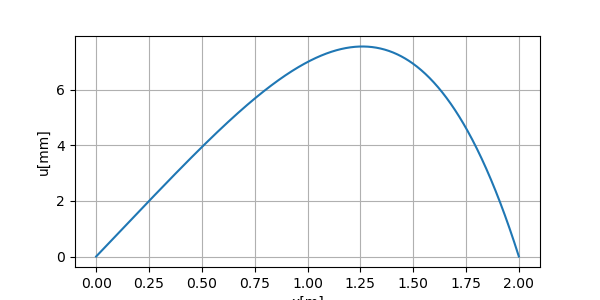
\includegraphics[scale=1]{Figures/2-Resmat/deslocamento_ex1.png}
            \caption{Campo de deslocamento do Exemplo 1}
            \label{fig:ex1_barra_ux}
        \end{figure}

        \begin{figure}[h!]
            \centering
            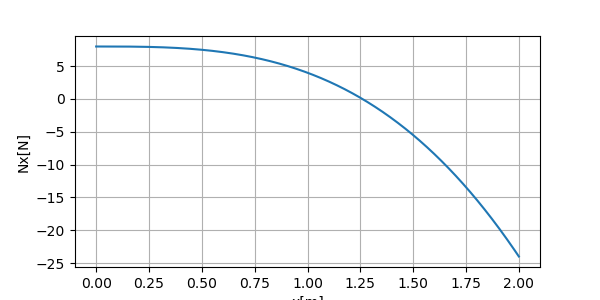
\includegraphics[scale=1]{Figures/2-Resmat/esforco_ex1.png}
            \caption{Esforço normal do Exemplo 1}
            \label{fig:ex1_barra_Nx}
        \end{figure}

        \begin{equation*}
            N_x(0) = 8 N
        \end{equation*}

        \begin{equation*}
            N_x(2) = -24 N
        \end{equation*}

        Na extremidade esquerda, pela convenção, o sinal positivo da condição de contorno é para a esquerda, portanto a força $N_x(0)$ deve apontar para a esquerda. Da mesma forma, na extremidade direita, o positivo é para a direita, portanto $N_x(2)$ deve apontar no sentido oposto, para a esquerda:

        \begin{equation*}
            R_A = -8N
        \end{equation*}

        \begin{equation*}
            R_B = -24N
        \end{equation*}

        Finalmente, se quiséssemos a deformação e a tensão, usaríamos:

        \begin{equation*}
            \sigma_{xx}(x) = \frac{N_x(x)}{A} = \frac{1}{A} \left[-4x^3 + 8\right]
        \end{equation*}

        \begin{equation*}
            \varepsilon_{xx}(x) = \frac{\sigma_{xx}}{E} = \frac{1}{EA} \left[-4x^3 + 8\right]
        \end{equation*}



        \subsubsection{Exemplo 2:}

        Encontre o campo de deslocamento, os esforços internos e as reações de apoio da barra da Figura \ref{fig:barra_ex2}. Suponha $EA = 10^{3} N$.

        \begin{figure}[h!]
            \centering
            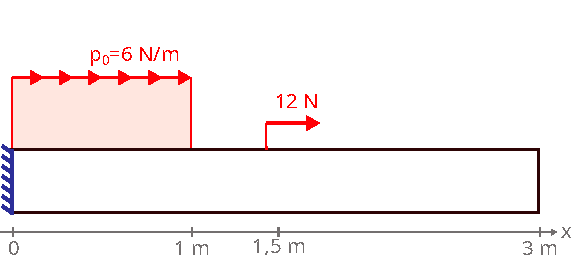
\includegraphics[scale=1]{Figures/2-Resmat/Exemplo2.pdf}
            \caption{Barra do Exemplo 2}
            \label{fig:barra_ex2}
        \end{figure}


        \subsubsection*{Solução}

        As condições de contorno neste problema são o engaste à esquerda ($u(0) = 0$) e a ausência de forças à direita ($N_x(3) = EAu'(3) = 0$).

        Para escrever $p(x)$, usaremos as funções de singularidade. A força distribuída pode ser escrita como a soma de uma força distribuída constante ao longo de todo o domínio com uma que anula com ela a partir de $x=1$ (Figura \ref{fig:barra_ex2_soma_forc}). A força concentrada é representada pelo delta de Dirac, multiplicado pela sua amplitude $12$ N:

        \begin{figure}[h!]
            \centering
            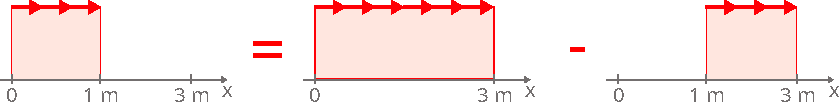
\includegraphics[scale=1]{Figures/2-Resmat/Soma_forc.pdf}
            \caption{Montagem da força distribuída}
            \label{fig:barra_ex2_soma_forc}
        \end{figure}

        \begin{equation*}
            p(x) = 6 - 6\sing{x}{1}{0} + 12\sing{x}{1,5}{-1}
        \end{equation*}


        Portanto, temos a equação diferencial:

        \begin{equation*}
            \left\{
            \begin{array}{l}
                EAu''(x) = -6 + 6\sing{x}{1}{0} - 12\sing{x}{1,5}{-1}\\
                u(0) = 0\\
                EAu'(3) = 0
            \end{array}
            \right.
        \end{equation*}


        Integrando sucessivamente:

        \begin{equation*}
            EAu''(x) = -6 + 6\sing{x}{1}{0} - 12\sing{x}{1,5}{-1}
        \end{equation*}

        \begin{equation*}
            EAu'(x) = -6x + 6\sing{x}{1}{1} - 12\sing{x}{1,5}{0} + C_1
        \end{equation*}

        \begin{equation*}
            EAu(x) = -3x^2 + 3\sing{x}{1}{2} - 12\sing{x}{1,5}{1} + C_1 x + C_2
        \end{equation*}

        \begin{equation*}
            u(x) = \frac{1}{EA} \left[-3x^2 + 3\sing{x}{1}{2} - 12\sing{x}{1,5}{1} + C_1 x + C_2\right]
        \end{equation*}

        Aplicando as condições de contorno:

        \begin{equation*}
            u(0) = 0 \rightarrow EAu(0) = C_2 = 0
        \end{equation*}

        \begin{equation*}
            EAu'(3) = 0 \rightarrow EAu'(3) = -6 \cdot 3 + 6\sing{3}{1}{1} - 12\sing{3}{1,5}{0} + C_1 = 0
        \end{equation*}

        \begin{equation*}
           -18 + 12 - 12 + C_1 = 0 \rightarrow C_1 = 18 N
        \end{equation*}


        Portanto:

        \begin{equation*}
            u(x) = \frac{1}{10^3} \left[-3x^2 + 3\sing{x}{1}{2} - 12\sing{x}{1,5}{1} + 18 x\right] [m]
        \end{equation*}

        \begin{equation*}
            u(x) = -3x^2 + 3\sing{x}{1}{2} - 12\sing{x}{1,5}{1} + 18 x [mm]
        \end{equation*}

        Perceba que $u(x)$ é uma função definida por trechos (já substituindo e fazendo as distributivas):

        \begin{equation*}
            u(x) = 
            \left\{
            \begin{array}{cl}
                -3x^2 + 18x &, x<1\\
                12x + 3 &, 1\leq x<1,5\\
                21 &, x\geq 1,5\\
            \end{array}
            \right. [mm]
        \end{equation*}


        O esforço normal:

        \begin{equation*}
            N_x(x) = EAu'(x) = -6x + 6\sing{x}{1}{1} - 12\sing{x}{1,5}{0} + 18
        \end{equation*}

        \begin{equation*}
            N_x(x) = 
            \left\{
            \begin{array}{cl}
                -6x + 18 &, x<1\\
                12 &, 1\leq x<1,5\\
                0 &, x\geq 1,5\\
            \end{array}
            \right. [N]
        \end{equation*}

        As Figuras \ref{fig:ex2_barra_ux} e \ref{fig:ex2_barra_Nx} mostram as curvas do deslocamento e esforço interno. A reação de apoio é dado por:

        \begin{figure}[h!]
            \centering
            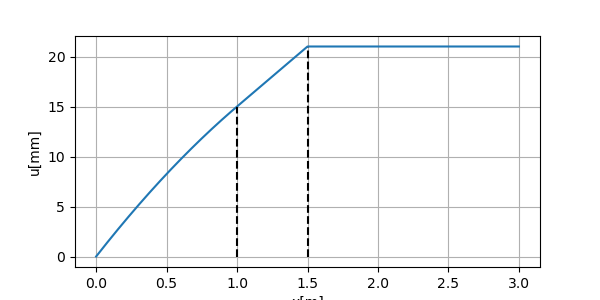
\includegraphics[scale=1]{Figures/2-Resmat/deslocamento_ex2.png}
            \caption{Campo de deslocamento do Exemplo 2}
            \label{fig:ex2_barra_ux}
        \end{figure}

        \begin{figure}[h!]
            \centering
            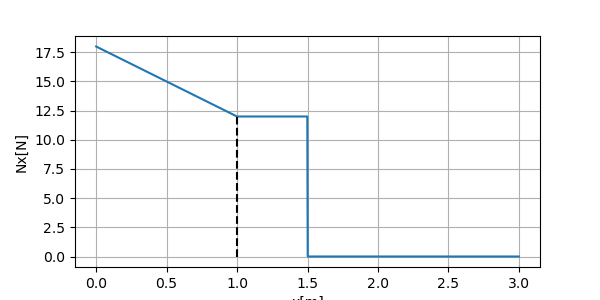
\includegraphics[scale=1]{Figures/2-Resmat/esforco_ex2.png}
            \caption{Esforço normal do Exemplo 2}
            \label{fig:ex2_barra_Nx}
        \end{figure}

        \begin{equation*}
            N_x(0) = -6 \cdot 0 + 18 = 18 N
        \end{equation*}

        Como a reação é positiva para a esquerda, na extremidade esquerda, então:

        \begin{equation*}
            R_A = -18 N
        \end{equation*}
    
        




	%LTeX: language=pt-br
% !TeX root = Apostila_IM381.tex

\cleardoublepage
\section{Solução aproximada de problema unidimensional - barra}

    Conforme mostrada na seção anterior, a equação diferencial da barra é dada pela equação:

    \begin{equation}
        E A \frac{d^2u}{dx^2} = -p(x),
    \end{equation}

    \noindent já considerando $E$, $A$ constantes.
    
    Nesta seção, vamos resolver esta equação de forma numérica. Dada a simplicidade desta equação, é possível avaliar a qualidade de nossa aproximação comparando-a com a solução analítica. Porém, de forma geral, não teremos uma solução de referência para avaliar nossa aproximação.

    O procedimento apresentado aqui é discutido para o caso específico da barra, porém ele pode ser usado para qualquer equação diferencial, ordinárias ou parciais. Na Seção \ref{sec:conducao}, ele será usado para o problema de condução de calor. Na Seção \ref{sec:estado_plano}, será usado no equilíbrio de estruturas elásticas.

    \subsection{Forma forte e forma fraca}

        Para exemplificar, resolveremos a seguinte equação diferencial com as seguintes condições de contorno (Figura \ref{fig:barra_exemplo_deducao}):

        \begin{figure}[h!]
            \centering
            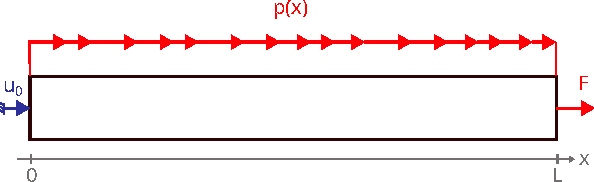
\includegraphics[scale=1]{Figures/2-Resmat/Barra_exemplo.pdf}
            \caption{Barra que servirá de exemplo.}
            \label{fig:barra_exemplo_deducao}
        \end{figure}

        \begin{equation}
            \begin{array}{c}
                E A \frac{d^2u}{dx^2} = -p(x)\\
                u(0) = u_0\\
                N_x(L) = \left.EA\frac{du}{dx}\right|_{x=L} = F
            \end{array}
        \end{equation}

        Embora analisemos este caso específico como um exemplo, o procedimento matemático é o mesmo para qualquer combinação de condições de contorno.

        A equação diferencial em sua forma original é chamada \textbf{forma forte}. Esta é a equação que obtemos diretamente das condições de equilíbrio do sistema ou de balanços de energia.

        A solução $u(x)$ dessa equação diferencial deve pertencer ao espaço de Sobolev $\mathcal{H}^1$ (Seção \ref{sec:algelin}). Mais especificamente, consideraremos aqui que a solução pertence ao espaço das funções com todas as derivadas contínuas (funções suaves) $C^\infty \subset \mathcal{H}^1$, e isso acontecerá se os esforços aplicados forem desta forma também.

        Portanto, definimos um espaço chamado espaço das funções teste $V$ (\textit{test functions}), que contém as soluções candidatas desta equação diferencial (incluindo sua solução):

        \begin{equation}
            V = \left\{u| u \in \mathcal{H}^1, u(0)=u_0 \right\}
        \end{equation}

        Na verdade, o espaço $V$ não é tecnicamente um espaço vetorial, pois ela não respeita o princípio da linearidade. Isto é, dadas duas funções $u_1,u_2 \in V$, $u_1(0) + u_2(0) \neq u_0$, logo, $u_1(x) + u_2(x) \notin V$. Entretanto, se pegarmos apenas os termos com $x \neq 0$ de cada função, ela se comportará como um espaço vetorial. Portanto, daqui em diante, trataremos ela como se fosse um espaço vetorial.

        Definiremos também um outro espaço, bastante similar, chamado espaço das funções peso $W$ (\textit{trial functions}). A diferença entre eles é que esté é realmente um espaço vetorial, com o(s) ponto(s) de condição de contorno de Dirichlet nulos:

        \begin{equation}
            W = \left\{w| w \in \mathcal{H}^1, w(0)=0 \right\}
        \end{equation}

        Podemos, então reescrever a equação diferencial da seguinte forma. Se a equação diferencial deve se anular, então o produto interno entre ela e uma função peso $w(x)$ também deve se anular, para qualquer $w(x) \in W$:

        \begin{equation}
            \int_0^L w(x)\left(EA\frac{d^2u}{dx^2} + p(x)\right) dx= 0 , \quad \forall w(x) \in W
        \end{equation}

        Suprimiremos a dependência de $x$ nas equações para simplificar a notação, porém ela permanece.

        Esta expressão é similar ao que se estuda na mecânica como o princípio do trabalho virtual. Este princípio enuncia que, dados os esforços externos e internos que mantenham o sistema em equilíbrio, se calcularmos o trabalho desses para qualquer campo de deslocamento (que obedeçam às restrições cinemáticas do problema), este deve ser nulo. Isto é, o trabalho das forças reais, quando sujeitas a um deslocamento virtual qualquer, deve ser nulo.

        Podemos reescrever a expressão acima, utilizando o procedimento de integração por partes:


        \begin{equation}
            \int_0^L EA w \frac{d^2u}{dx^2} dx + \int_0^Lwp(x) dx = 0
        \end{equation}

        \begin{equation}
            -\int_0^L EA \frac{dw}{dx} \frac{du}{dx} dx  + \left[EA w \frac{du}{dx}\right]_0^L+ \int_0^Lwp(x) dx = 0
        \end{equation}

        \begin{equation}
            \int_0^L EA \frac{dw}{dx} \frac{du}{dx} dx  = F w(L) + \int_0^Lwp(x) dx , \quad \forall w(x) \in W
            \label{eq:forma_fraca}
        \end{equation}

        Esta expressão é chamada \textbf{forma fraca}. As formas fraca e forte são equivalentes, mesmo que os nomes induzam o leitor a achar que uma delas se sobressaia a outra de alguma forma. Ambas descrevem de forma única a equação diferencial, e existe apenas uma única solução para ambas. Na forma fraca, entretanto, essa unicidade de solução só é garantida pelo fato da função peso poder assumir qualquer função em $W$.

        Na forma fraca, as condições de contorno de Dirichlet ainda devem aparecer explicitamente na definição de $u(x)$, entretanto, as condições de Neumann aparecem implicitamente nos termos de contorno que aparecem da integração por partes.

        Muitas vezes, podemos encontrar a forma fraca representada a partir de operadores bidirecionais, isto é:

        \begin{equation}
            a(w,u)  = (w,p)
        \end{equation}

        \noindent no qual $a(w,u)$ é um operador comutativo, que representa a integral à esquerda da igualdade. Já o termo $(w,p)$ representa os termos de esforços que aparecem do lado direito da igualdade.

        \subsubsection*{Equivalência entre as formas forte e fraca}

        Conforme dito na seção anterior, as formas fraca e forte são equivalentes, e encontrar a solução que satisfaça uma é equivalente a encontrar a solução da outra. A prova de que a solução da forma forte é solução da forma fraca já foi demonstrada na seção anterior, através da integração por partes. Agora, nos preocupamos em fazer o caminho inverso, provar que a solução da forma fraca implica na solução da forma forte.

        Suponha que $u(x)$ seja solução da forma fraca. Logo $u(0) = u_0$ ($w(0) = 0$) e:

        \begin{equation*}
            \int_0^L EA \frac{dw}{dx} \frac{du}{dx} dx  = F w(L) + \int_0^Lwp(x) dx , \quad \forall w(x) \in W
        \end{equation*}

        Aplicando integração por partes:

        \begin{equation*}
            -\int_0^L EA w \frac{d^2u}{dx^2} dx +  \left[EA w \frac{du}{dx}\right]_0^L = F w(L) + \int_0^Lwp(x) dx , \quad \forall w(x) \in W
        \end{equation*}

        \begin{equation*}
            \int_0^L EA w(x) \left(\frac{d^2u}{dx^2} + p(x)\right) dx +  w(L)\left[F - EAu'(L) \right] = 0 , \quad \forall w(x) \in W
            \label{eq:fraca_igual_forte}
        \end{equation*}

        Para que esta igualdade se verifique, basta que:

        \begin{equation*}
            I = \frac{d^2u}{dx^2} + p(x) = 0
        \end{equation*}

        \begin{equation*}
            II = F - EA u'(L) = 0
        \end{equation*}

        Como a forma fraca é válida para qualquer $w(x) \in W$, então podemos verificar para um exemplo de $w(x)$:

        \begin{equation*}
            w(x) = \phi(x)\left(\frac{d^2u}{dx^2} + p(x)\right)
        \end{equation*}

        \noindent no qual $\phi(x)$ é uma função suave no intervalo $(0,L)$ e satisfaz $\phi(0) = \phi(L) = 0$. Por exemplo, se $\phi(x) = x(L-x)$, então $w(0) = 0$, logo $w(x) \in W$. Inserindo este valor na Eq. \eqref{eq:fraca_igual_forte}:

        \begin{equation*}
            \int_0^L EA \phi\left(\frac{d^2u}{dx^2} + p(x)\right)^2 dx + 0 = 0
        \end{equation*}

        Como $\phi(x) >0$ e $\left(\frac{d^2u}{dx^2} + p(x)\right)^2 \geq 0$ para qualquer $x$ entre $0$ e $L$, então para que a integral se anule, $\frac{d^2u}{dx^2} + p(x) = 0$ para todo $x$ entre $0$ e $L$.

        Agora que provamos que $I=0$, a Eq. \eqref{eq:fraca_igual_forte} pode ser reduzida a:

        \begin{equation*}
           w(L)\left[F - EAu'(L) \right] = 0 , \quad \forall w(x) \in W
        \end{equation*}

        Como $W$ não impõe nenhuma restrição no valor de $w(L)$, então este ainda pode assumir qualquer valor. Portanto, a única forma dessa igualdade ser verificada é se:

        \begin{equation*}
            F - EAu'(L) = 0 
        \end{equation*}

        Portanto, $II = 0$ é verificado. Desta forma, com as expressões de $I$, $II$ e da condição de Dirichlet imposta em $V$, temos que a solução da forma fraca também é solução da forma forte.



    \subsection{Método dos Resíduos Ponderados e Método de Galerkin}

        Até o momento, trabalhamos apenas com soluções exatas da equação diferencial. Salvo casos muito específicos, normalmente não será viável ou possível resolver o problema desta forma. Portanto, propomos aqui um método para aproximar a solução.

        Suponha que agora, desejamos obter uma solução aproximada $u^h(x)$ da equação diferencial. Esta solução pertencerá a um espaço $V^h$. Isto é:

        \begin{equation}
            u^h(x) \in V^h \subset V
        \end{equation}

        O espaço original $V$ possui dimensão infinita. Definimos o subespaço $V^h$ tal que este possua dimensão finita.

        Similarmente, definimos uma função peso $w^h(x) \in W^h \subset W$.

        O \textbf{Método dos Resíduos Ponderados} implica em obter a função $u^h(x)$ que zere o resíduo de seu produto interno com qualquer $w^h(x),$ isto é:

        \begin{equation}
            \int_0^L w^h(x)\left(EA\frac{d^2u^h}{dx^2} + p(x)\right) dx= r = 0 , \quad \forall w^h(x) \in W^h
        \end{equation}

        Em um procedimento similar ao anterior, obtemos a equação na forma:

        \begin{equation}
            \int_0^L EA \frac{dw^h}{dx} \frac{du^h}{dx} dx  = N_x(L) w^h(L) - N_x(0) w^h(0) + \int_0^Lw^hp(x) dx , \quad \forall w^h(x) \in W
        \end{equation}

        Antes de prosseguir, vamos fazer algumas considerações sobre as fontes de erro na aproximação da nossa solução. Primeiramente, por se tratar de um subespaço, a solução aproximada será a mais próxima possível da projeção da solução real neste mesmo subespaço (análogo à projeção de vetores, Figura \ref{fig:projecao}). Entretanto, ainda haverá erros devido aos termos fora do subespaço de aproximação.

        \begin{figure}[h!]
            \centering
            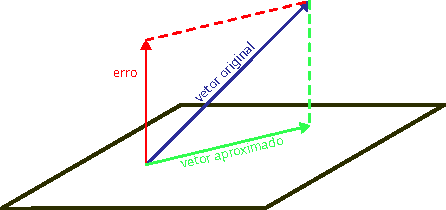
\includegraphics[scale=1]{Figures/3-Barra/Projecao.pdf}
            \caption{Exemplo de projeção de vetor em um subespaço: projeção de um vetor de $\mathbb{R}^3$ em $\mathbb{R}^2$}
            \label{fig:projecao}
        \end{figure}

        Sobre as condições de contorno, as condições de Dirichlet continuam sendo aplicadas explicitamente em $u^h(x)$, portanto, elas continuam exatas. Entretanto, as condições de Neumann aparecem implicitamente nos termos da integração por partes. Isto é, as condições de Neumann também podem não ser exatas.

        A forma mais usual, no contexto de elementos finitos, para continuar a solução dessa equação é utilizando o \textbf{Método de Galerkin}. Para este, assumimos que os subespaços $V^h$ e $W^h$ são iguais (salvo o termo de condição de contorno). Isto é $V^h = W^h$.

    \subsection{Funções de forma}

        Como os espaços $V^h$ e $W^h$ são finitos, podemos escrever qualquer termo deles como uma combinação linear de uma base que forme este espaço. Chamaremos estas funções que formam uma base desse espaço \textbf{funções de forma}, $N_1(x), N_2(x), \cdots, N_n(x)$. Portanto, podemos escrever o deslocamento e a função peso como:

        \begin{equation}
            u^h(x) = a_1 N_1(x) + a_2 N_2(x) + \cdots + a_n N_n(x) = \sum_{i=1}^n a_i N_i(x) =
            \begin{bmatrix}
                N_1 & 
                N_2 &
                \cdots&
                N_n
            \end{bmatrix}
            \begin{Bmatrix}
                a_1 \\ 
                a_2 \\
                \vdots\\
                a_n
            \end{Bmatrix} 
            = \mathbf{N} \mathbf{a}
        \end{equation}

        \begin{equation}
            w^h(x) = b_1 N_1(x) + b_2 N_2(x) + \cdots + b_n N_n(x) = \sum_{i=1}^n b_i N_i(x) = \mathbf{N} \mathbf{b}
        \end{equation}

        Substituíndo essas expressões na forma fraca:

        \begin{equation*}
            \int_0^L EA \left(\sum_{i=1}^n b_i\frac{dN_i}{dx}\right) \left(\sum_{j=1}^n a_j\frac{dN_j}{dx}\right) dx = \left(\sum_{i=1}^n b_i N_i(L)\right)F + \int_0^L \left(\sum_{i=1}^n b_i N_i(x)\right) p(x) dx
        \end{equation*}

        \begin{equation*}
            \sum_{i=1}^n b_i \left( \sum_{j=1}^n a_j\int_0^L EA \frac{dN_i}{dx} \frac{dN_j}{dx} dx \right) = \sum_{i=1}^n b_i \left(N_i(L) F + \int_0^L N_i(x) p(x) dx\right)
        \end{equation*}

        Como a equação deve se satisfazer para qualquer $w^h(x)$, então ela deve se satisfazer para qualquer combinação de $b_i$. Portanto, igualamos os termos com mesmo $b_i$ para obtermos um sistema de $n$ equações:

        \begin{equation*}
            \sum_{j=1}^n \left(\int_0^L EA \frac{dN_i}{dx} \frac{dN_j}{dx} dx\right) a_j = N_i(L) F + \int_0^L N_i(x) p(x) dx, \quad i=1,2\cdots, n
        \end{equation*}

        Este procedimento normalmente é representado em equação matricial, ficando da seguinte forma:

        \begin{equation*}
            \left(\int_0^L 
            \begin{Bmatrix}
            \frac{dN_1}{dx}\\
            \frac{dN_2}{dx}\\
            \vdots\\
            \frac{dN_n}{dx}\\
            \end{Bmatrix}
            EA
            \begin{bmatrix}
            \frac{dN_1}{dx} &
            \frac{dN_2}{dx} &
            \cdots &
            \frac{dN_n}{dx}
            \end{bmatrix} dx\right) \begin{Bmatrix}
            a_1\\
            a_2\\
            \vdots\\
            a_n\\
            \end{Bmatrix} = \mathbf{N}^T(L) F + \int_0^L \mathbf{N}^T p(x) dx
        \end{equation*}

        \begin{equation*}
            \left(\int_0^L 
            \mathbf{B}^T
            \mathbf{D}
            \mathbf{B} dx \right)
            \mathbf{a} = \mathbf{N}^T(L) F + \int_0^L \mathbf{N}^T p(x) dx
        \end{equation*}


        Chega-se portanto a um sistema linear. A matriz que aparece à esquerda é chamada \textbf{matriz de rigidez}:

        \begin{equation}
            \mathbf{K} = \int_0^1 
            \mathbf{B}^T
            \mathbf{D}
            \mathbf{B} dx = 
            \begin{bmatrix}
                K_{11} & K_{12} & \cdots & K_{1n}\\
                K_{21} & K_{22} & \cdots & K_{2n}\\
                \vdots & \vdots & \ddots & \vdots\\
                K_{n1} & K_{n2} & \cdots & K_{nn}\\
            \end{bmatrix}
        \end{equation}

        Esta matriz é uma matriz quadrada, simétrica e semi-positivo definida. Ela normalmente é escrita como um produto entre uma matriz $\mathbf{B}$ e uma matriz $\mathbf{D}$. Estes representam, respectivamente, as relações cinemáticas e as propriedades do modelo de material usados no problema. De forma geral, para qualquer caso podemos escrever a matriz desta forma, variando esses termos de acordo com a física e o material.

        Do lado direito da igualdade, aparece o \textbf{vetor de forças nodais}:

        \begin{equation}
            \mathbf{f} = \mathbf{N}^T(1) F + \int_0^1 \mathbf{N}^T p(x) dx =
            \begin{Bmatrix}
                F_1\\
                F_2\\
                \vdots\\
                F_n
            \end{Bmatrix}
        \end{equation}

        Finalmente, as incógnitas do problema estão no vetor de \textbf{deslocamentos nodais}:

        \begin{equation*}
            \mathbf{a} =
            \begin{Bmatrix}
                a_1\\
                a_2\\
                \vdots\\
                a_n
            \end{Bmatrix}
        \end{equation*}

        Portanto, reduzimos o problema a um sistema linear:

        \begin{equation}
            \mathbf{K} \mathbf{a} = \mathbf{f} 
        \end{equation}

        Resolvendo este, obtemos os coeficientes $a_i$ e, portanto o campo de deslocamento aproximado $u^h(x)$.
    
    \subsection{Considerações sobre condições de contorno e a solução}
    \label{sec:condicao_contorno}

        Para aplicar as condições de contorno no sistema, normalmente já partimos do sistema montado.

        Para as condições de Neumann, isto é, condições na derivada do deslocamento, elas já aparecem do lado direito da expressão da forma fraca. No caso da barra, surge, por exemplo, no termo:

        \begin{equation}
            \mathbf{N}^T(1) F
        \end{equation}

        Portanto, deve-se avaliar todas as funções de forma no ponto de aplicação da força concentrada, que por sua vez, retorna um vetor:

        \begin{equation}
            \mathbf{N}^T(1) F = \begin{Bmatrix}
                N_1(1)\\
                N_2(1)\\
                \vdots\\
                N_n(1)
            \end{Bmatrix}
            F
        \end{equation}

        Este vetor é somado ao vetor de forças $\mathbf{f}$. Como veremos na próxima seção, em alguns pontos do domínio, chamados \textbf{nós}, todas as funções de forma são nulas, exceto uma, que assume valor unitário. Portanto, uma força aplicada neste nó aparece como:

        \begin{equation}
            \mathbf{N}^T(1) F = \begin{Bmatrix}
                0\\
                0\\
                \vdots\\
                F
            \end{Bmatrix}
        \end{equation}

        Para as condições de Dirichlet, temos que o deslocamento em algum ponto será dado, portanto:

        \begin{equation*}
            u(0) = u_0
        \end{equation*}

        \begin{equation*}
             \begin{bmatrix}
                N_1(0) & 
                N_2(0) &
                \cdots&
                N_n(0)
            \end{bmatrix}
            \begin{Bmatrix}
                a_1 \\ 
                a_2 \\
                \vdots\\
                a_n
            \end{Bmatrix}  = u_0
        \end{equation*}

        Novamente, essas condições de contorno devem ser aplicadas usualmente em nós, nos quais apenas uma função de forma será não nula, portanto, assumindo que $N_1(0) = 1$ e os outros nulos:

        \begin{equation*}
            a_1 = u_0
        \end{equation*}

        O sistema global, portanto, fica:

        \begin{equation*}
             \begin{bmatrix}
                K_{11} & K_{12} & \cdots & K_{1n}\\
                K_{21} & K_{22} & \cdots & K_{2n}\\
                \vdots & \vdots & \ddots & \vdots\\
                K_{n1} & K_{n2} & \cdots & K_{nn}\\
            \end{bmatrix}
            \begin{Bmatrix}
                u_0 \\ 
                a_2 \\
                \vdots\\
                a_n
            \end{Bmatrix}
            =
             \begin{Bmatrix}
                F_1 + R\\
                F_2\\
                \vdots\\
                F_n
            \end{Bmatrix}
        \end{equation*}

        \noindent no qual aparece uma reação de apoio $R$ na mesma linha (seguindo a lógica da condição de Neumann acima, porém em x = 0).

        A primeira linha desse sistema envolve uma incógnita a mais ($R$), portanto, podemos removê-la. Se quisermos calcular $R$ após resolver o sistema, basta voltarmos a esta linha:

        \begin{equation*}
            K_{11}u_0  + K_{12}a_2 + \cdots + K_{1n}a_n = F_1 + R
        \end{equation*}

        \begin{equation*}
            \begin{bmatrix}
                K_{21} & K_{22} & \cdots & K_{2n}\\
                \vdots & \vdots & \ddots & \vdots\\
                K_{n1} & K_{n2} & \cdots & K_{nn}\\
            \end{bmatrix}
            \begin{Bmatrix}
                u_0\\
                a_2 \\
                \vdots\\
                a_n
            \end{Bmatrix}
            =
             \begin{Bmatrix}
                F_2\\
                \vdots\\
                F_n
            \end{Bmatrix}
        \end{equation*}

        Entretanto, agora temos um sistema retangular. Porém, conhecemos o valor de $a_1$, que deve ser $u_0$, então podemos reescrever o sistema como:

        \begin{equation*}
            \begin{Bmatrix}
                K_{11}\\
                K_{21} \\
                \vdots\\
                K_{n1}
            \end{Bmatrix}
            u_0
            +
            \begin{bmatrix}
                K_{22} & K_{23} & \cdots & K_{2n}\\
                \vdots & \vdots & \ddots & \vdots\\
                K_{n2} & K_{n3} & \cdots & K_{nn}\\
            \end{bmatrix}
            \begin{Bmatrix}
                a_2 \\
                \vdots\\
                a_n
            \end{Bmatrix}
            =
             \begin{Bmatrix}
                F_2\\
                \vdots\\
                F_n
            \end{Bmatrix}
        \end{equation*}

        \begin{equation*}
            \begin{bmatrix}
                K_{22} & K_{23} & \cdots & K_{2n}\\
                \vdots & \vdots & \ddots & \vdots\\
                K_{n2} & K_{n3} & \cdots & K_{nn}\\
            \end{bmatrix}
            \begin{Bmatrix}
                a_2 \\
                \vdots\\
                a_n
            \end{Bmatrix}
            =
             \begin{Bmatrix}
                F_2\\
                \vdots\\
                F_n
            \end{Bmatrix}
            -
            \begin{Bmatrix}
                K_{11}\\
                K_{21} \\
                \vdots\\
                K_{n1}
            \end{Bmatrix}
            u_0
        \end{equation*}

        \noindent que é um sistema linear quadrado.

        Resumindo, de forma algorítmica, fazemos o seguinte procedimento:

        \begin{enumerate}
            \item Identificamos a linha e coluna correspondente ao coeficiente que conhecemos devido à condição de contorno
            \item ``Cortamos'' esta linha e esta coluna da matriz de rigidez e a linha do vetor de forças. A matriz de rigidez agora deve ser quadrada e menor que antes.
            \item Se a condição de contorno for nula ($u_0=0$), continuar. Caso contrário, subtrair no vetor de forças a coluna removida da matriz de rigidez multiplicada pela condição de contorno.
            \item Prosseguir na resolução do sistema. 
        \end{enumerate}




    \subsection{Condiderações sobre o método}

        O procedimento mostrado nessa seção já descreve totalmente como partir da equação diferencial e chegar ao sistema linear que nos fornece os coeficientes da solução aproximada. Este procedimento pode ser aplicado em qualquer PVI, sejam equações diferenciais ordinárias, sejam equações diferenciais parciais. Com as ferramentas apresentadas até aqui, o leitor já deve ser capaz de propor e resolver alguns problemas, mesmo que esta solução aproximada não seja a melhor, ou mesmo que o procedimento não seja tão computacionalmente barato quanto ele pode ser.

        O procedimento geral para qualquer problema físico é o mesmo, partir da forma forte, definir funções peso e fazer integração por partes (Teorema de Green em 2D e 3D) para encontrar a forma fraca. Aplicar o Método dos Resíduos Ponderados, propondo um subespaço para as soluções aproximadas. Aplicar o Método de Galerkin, propondo as mesmas funções de forma para o espaço das funções peso aproximadas. Fazer a manipulação algébrica necessária para reduzir o problema a um sistema linear. Resolvendo o sistema, obtém-se uma solução aproximada.

        Nos próximos capítulos, formalizaremos este método, sistematizando-o. Definiremos o tipo de função de forma mais usual. Veremos como definir essas funções de forma para podemrmos utilizá-las de forma intercambiável em qualquer domínio de integração, possibilitando a aplicação dessas mesmo em geometrias complexas. Estudaremos um método simples e barato para fazer as integrações necessárias para a matriz de rigidez e vetor de forças.

	%LTeX: language=pt-br
% !TeX root = Apostila_IM381.tex

\cleardoublepage
\section{Elemento de barra}
\label{sec:elemento_barra}
    Na seção anterior, definimos os procedimentos para partirmos da equação diferencial do problema para chegarmos a um sistema linear que resulta numa solução aproximada para o problema. Nesta seção, definiremos as características que caracterizam o método dos elementos finitos. Mostraremos como sistematizar o procedimento da seção anterior.

    \subsection{Funções de forma definidas por trecho}

        Como um método numérico, a força do Método dos Elementos Finitos (MEF) está em sua aplicabilidade mesmo em problemas de alta complexidade geométrica. Mesmo componentes com geometrias bastante irregulares podem ter seu movimento descrito pelo MEF. Para tanto, é necessário sistematizar como definir as funções de forma que aproximam a solução.

        Não é fácil (e muitas vezes não é possível), definir um conjunto de funções no domínio de análise que obedeçam as condições de contorno de Dirichlet e que sejam linearmente independentes. Desta forma, o mais simples é subdividir esse domínio, e definir as funções apenas dentro de cada subdomínio. Cada subdomínio desses é chamado \textbf{elemento}. Ao conjunto de todos os elementos, damos o nome de \textbf{malha}.

        Desta forma, subdividimos o domínio de análise em elementos, isto é, discretizamos o domínio de análise em uma malha de elementos finitos (Figura \ref{fig:discretizacao}). Este procedimento de discretização por si só já pode gerar erros, visto que estamos aproximando as superfícies da estrutura. As funções de forma são definidas tais que cada uma delas apenas assume valores diferentes de zero em um único elemento. Considere o domínio da Figura \ref{fig:malha_barra} para a solução do problema da barra. Dividimos este domínio em quatro elementos. As funções de forma mais usuais são a ``função chapéu'', que recebe este nome devido a sua forma (Figura \ref{fig:malha_barra_forma}). Os pontos de interface entre cada elemento são chamados \textbf{nós}.

        \begin{figure}[h!]
            \centering
            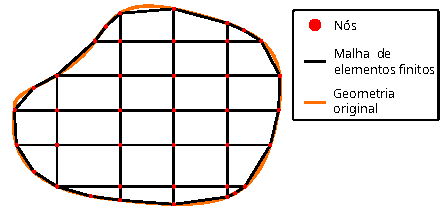
\includegraphics[scale=1]{Figures/4-Elemento_barra/Malha.pdf}
            \caption{Discretização em elementos finitos quadrangulares de uma geometria.}
            \label{fig:discretizacao}
        \end{figure}


        \begin{figure}[h!]
            \centering
            \begin{subfigure}{0.99\textwidth}
                \centering
                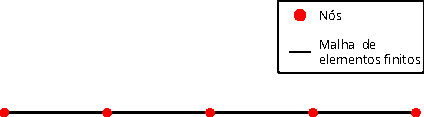
\includegraphics[scale=1]{Figures/4-Elemento_barra/Malha_Barra.pdf}
                \caption{}
                \label{fig:malha_barra}
            \end{subfigure}
            \\
            \begin{subfigure}{0.99\textwidth}
                \centering
                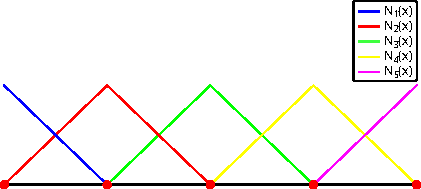
\includegraphics[scale=1]{Figures/4-Elemento_barra/Barra_Funcao_Forma.pdf}
                \caption{}
                \label{fig:malha_barra_forma}
            \end{subfigure}
            \caption{Discretização da barra. (a) Elementos e nós de um sistema de elementos de barra, (b) funções de forma ``chapéu''.}
            \label{fig:malha_barra_tot}
        \end{figure}

        Matematicamente, uma função chapéu qualquer pode ser descrita como:

        \begin{equation}
            N_i(x) = 
            \left\{
            \begin{array}{cl}
                \frac{x-x_{i-1}}{h_{i-1}} & x_{i-1} \leq x \leq x_i\\
                \frac{x_{i+1}-x}{h_i} & x_i \leq x \leq x_{i+1}\\
                0 & \text{qualquer outro ponto}\\
            \end{array}
            \right.
        \end{equation}

        \noindent no qual $h_i = x_{i+1}-x_i$ e $h_{i-1} = x_i -x_{i-1}$.

        Conforme vimos na seção anterior, precisaremos também da derivada dessa função:

        \begin{equation}
            \frac{dN_i}{dx} = 
            \left\{
            \begin{array}{cl}
                \frac{1}{h_{i-1}} & x_{i-1} \leq x \leq x_i\\
                \frac{-1}{h_i} & x_i \leq x \leq x_{i+1}\\
                0 & \text{qualquer outro ponto}\\
            \end{array}
            \right.
        \end{equation}

        Desta forma, conseguimos encontrar a matriz de rigidez do sistema resolvendo a integral:

        \begin{equation}
            \mathbf{K} = \int_0^L EA 
            \begin{Bmatrix}
            \frac{dN_1}{dx}\\
            \frac{dN_2}{dx}\\
            \vdots\\
            \frac{dN_n}{dx}\\
            \end{Bmatrix}
            \begin{bmatrix}
            \frac{dN_1}{dx} &
            \frac{dN_2}{dx} &
            \cdots &
            \frac{dN_n}{dx}
            \end{bmatrix} dx
            = \int_0^L \mathbf{B}^T \mathbf{D}\mathbf{B} dx
        \end{equation}

        \subsubsection*{Particularidade da função chapéu}

            O deslocamento aproximado pode ser reconstruído por:

            \begin{equation}
                u^h(x) = a_1 N_1(x) + a_2 N_2(x) + \cdots + a_n N_n(x)
            \end{equation}

            Considere agora o deslocamento em um nó $x_i$, apenas uma função chapéu terá valor diferente de zero, e este será unitário, isto é:

            \begin{equation}
                u^h(x) = a_i
            \end{equation}

            Portanto, ao usar funções de forma com esta propriedade, podemos chamar o vetor $\mathbf{a}$ de vetor de deslocamento nodais, e cada termo desse vetor representará o deslocamento de cada um dos nós.

            Entretanto, é precso se lembrar sempre que o MEF é um método para obter a solução aproximada ao longo de \textbf{todo} o domínio de análise, não apenas dos nós. Portanto, qualquer análise a ser feita em cima deste método \textbf{deve} considerar as interpolações em cada elemento.

            Outra particularidade na solução do problema de barra é a propriedade da \textbf{superconvergência} (Apêndice \ref{app:superconvergencia}). Para este problema, os deslocamentos nodais serão exatos, isto é, os coeficientes encontrados no sistema linear serão iguais aos deslocamentos da solução analítica (salvo erros numéricos). Note que, para um caso geral de elementos finitos, essa propriedade não se observa, isto é, \textbf{os deslocamentos nodais são aproximados.}

        \subsubsection*{Exemplo:}

            Considere uma barra com $L=1$ m com uma força distribuída uniforme de $4$ N/m e uma força concentrada de $10$ N na extremidade direita. A barra está apoiada na extremidade esquerda. Considere $E = 10^9$ Pa e $A = 10^{-6}$ m$^2$.

            Suas funções de forma serão:

            \begin{equation*}
            N_1(x) = 
            \left\{
            \begin{array}{cl}
                1-2x & 0 \leq x \leq 0.5\\
                0 & \text{qualquer outro ponto}\\
            \end{array}
            \right.
            \rightarrow
            \frac{dN_1}{dx} = 
            \left\{
            \begin{array}{cl}
                -2 & 0 \leq x \leq 0.5\\
                0 & \text{qualquer outro ponto}\\
            \end{array}
            \right.
        \end{equation*}

        \begin{equation*}
            N_2(x) = 
            \left\{
            \begin{array}{cl}
                2x & 0 \leq x \leq 0.5\\
                2-2x & 0.5 \leq x \leq 1\\
                0 & \text{qualquer outro ponto}\\
            \end{array}
            \right.
            \rightarrow
            \frac{dN_2}{dx} = 
            \left\{
            \begin{array}{cl}
                2 & 0 \leq x \leq 0.5\\
                -2 & 0.5 \leq x \leq 1\\
                0 & \text{qualquer outro ponto}\\
            \end{array}
            \right.
        \end{equation*}

        \begin{equation*}
            N_3(x) = 
            \left\{
            \begin{array}{cl}
                2x-1 & 0.5 \leq x \leq 1\\
                0 & \text{qualquer outro ponto}\\
            \end{array}
            \right.
            \rightarrow
            \frac{dN_3}{dx} = 
            \left\{
            \begin{array}{cl}
                2 & 0.5 \leq x \leq 1\\
                0 & \text{qualquer outro ponto}\\
            \end{array}
            \right.
        \end{equation*}

        Com isso, podemos encontrar a matriz de rigidez. Lembre-se que uma integral pode ser dividida como a soma de integrais cujos domínios de integração se somem no domínio original.

        \begin{equation*}
            \mathbf{K} = \int_0^1 EA 
            \begin{Bmatrix}
            \frac{dN_1}{dx}\\
            \frac{dN_2}{dx}\\
            \frac{dN_3}{dx}\\
            \end{Bmatrix}
            \begin{bmatrix}
            \frac{dN_1}{dx} &
            \frac{dN_2}{dx} &
            \frac{dN_3}{dx}
            \end{bmatrix} dx
        \end{equation*}

        \begin{equation*}
            \mathbf{K} = \int_0^{0.5} EA 
            \begin{Bmatrix}
            \frac{dN_1}{dx}\\
            \frac{dN_2}{dx}\\
            \frac{dN_3}{dx}\\
            \end{Bmatrix}
            \begin{bmatrix}
            \frac{dN_1}{dx} &
            \frac{dN_2}{dx} &
            \frac{dN_3}{dx}
            \end{bmatrix} dx + \int_{0.5}^{1} EA 
            \begin{Bmatrix}
            \frac{dN_1}{dx}\\
            \frac{dN_2}{dx}\\
            \frac{dN_3}{dx}\\
            \end{Bmatrix}
            \begin{bmatrix}
            \frac{dN_1}{dx} &
            \frac{dN_2}{dx} &
            \frac{dN_3}{dx}
            \end{bmatrix} dx
        \end{equation*}

        \begin{equation*}
            \mathbf{K} = \int_0^{0.5} EA 
            \begin{Bmatrix}
            -2\\
            2\\
            0\\
            \end{Bmatrix}
            \begin{bmatrix}
            -2 &
            2 &
            0
            \end{bmatrix} dx + \int_{0.5}^{1} EA 
            \begin{Bmatrix}
            0\\
            -2\\
            2\\
            \end{Bmatrix}
            \begin{bmatrix}
            0 &
            -2 &
            2
            \end{bmatrix} dx
        \end{equation*}

        \begin{equation*}
            \mathbf{K} = \int_0^{0.5} EA 
            \begin{bmatrix}
            4 & -4 & 0\\
            -4 & 4 & 0\\
            0 & 0 & 0
            \end{bmatrix} dx + 
            \int_{0.5}^{1} EA 
            \begin{bmatrix}
            0 & 0 & 0 \\
            0 & 4 & -4 \\
            0 & -4 & 4
            \end{bmatrix} dx
        \end{equation*}

        \begin{equation*}
            \mathbf{K} = 10^3 
            \begin{bmatrix}
            2 & -2 & 0\\
            -2 & 2 & 0\\
            0 & 0 & 0
            \end{bmatrix} + 
            10^3 
            \begin{bmatrix}
            0 & 0 & 0 \\
            0 & 2 & -2 \\
            0 & -2 & 2
            \end{bmatrix}
        \end{equation*}


        \begin{equation*}
            \mathbf{K} = 
            10^3\begin{bmatrix}
                2 & -2 & 0\\
                -2 & 4 & -2\\
                0 & -2 & 2
            \end{bmatrix}
        \end{equation*}

        Seguiremos de forma análoga para a força. Entretanto, a extremidade direita se encontra carregada com $F = 10$ N. Na extremidade esquerda, haverá a reação de apoio desconhecida $R_x$.

        \begin{equation*}
            \mathbf{f} = \mathbf{N}^T(1) F + \mathbf{N}^T(0) R_x + \int_0^1 \mathbf{N}^T p(x) dx
        \end{equation*}

        \begin{equation*}
            \mathbf{N}^T =
            \begin{Bmatrix}
                N_1(x) \\
                N_2(x) \\
                N_3(x)
            \end{Bmatrix}
        \end{equation*}

        \begin{equation*}
            \mathbf{f} = 
            \begin{Bmatrix}
                0 \\
                0 \\
                1
            \end{Bmatrix} F 
            + \begin{Bmatrix}
                1 \\
                0 \\
                0
            \end{Bmatrix} R_x 
            + \int_{0}^{0.5} 
            \begin{Bmatrix}
                1-2x\\
                2x \\
                0
            \end{Bmatrix} 4 dx 
            + \int_{0.5}^{1}
            \begin{Bmatrix}
                0\\
                2-2x \\
                2x-1
            \end{Bmatrix} 4 dx
        \end{equation*}

        \begin{equation*}
            \mathbf{f} = 
            \begin{Bmatrix}
                0 \\
                0 \\
                F
            \end{Bmatrix}
            + \begin{Bmatrix}
                R_x \\
                0 \\
                0
            \end{Bmatrix}
            + \left.
            \begin{Bmatrix}
                4x-4x^2\\
                4x^2 \\
                0
            \end{Bmatrix}\right|_{0}^{0.5}
            + \left.
            \begin{Bmatrix}
                0\\
                8x-4x^2 \\
                4x^2-4x
            \end{Bmatrix} \right|_{0.5}^{1}
        \end{equation*}

        \begin{equation*}
            \mathbf{f} = 
            \begin{Bmatrix}
                0 \\
                0 \\
                10
            \end{Bmatrix}
            + \begin{Bmatrix}
                R_x \\
                0 \\
                0
            \end{Bmatrix}
            +
            \begin{Bmatrix}
                1\\
                1\\
                0
            \end{Bmatrix}
            +
            \begin{Bmatrix}
                0\\
                4 \\
                0
            \end{Bmatrix}
            -
            \begin{Bmatrix}
                0\\
                3 \\
                -1
            \end{Bmatrix}
        \end{equation*}

        \begin{equation*}
            \mathbf{f} = 
            \begin{Bmatrix}
                1 + R_x\\
                2\\
                11
            \end{Bmatrix}
        \end{equation*}

        Portanto, o sistema linear fica da forma:

        \begin{equation*}
            \mathbf{K} \mathbf{a} = \mathbf{f} 
        \end{equation*}

        \begin{equation*}
            10^3\begin{bmatrix}
                2 & -2 & 0\\
                -2 & 4 & -2\\
                0 & -2 & 2
            \end{bmatrix}
            \begin{Bmatrix}
                a_1\\
                a_2\\
                a_3
            \end{Bmatrix}
            =
            \begin{Bmatrix}
                1 + R_x\\
                2\\
                11
            \end{Bmatrix}
        \end{equation*}

        Para aplicar as condições de contorno, usamos os procedimentos da Seção \ref{sec:condicao_contorno}, isto é, ``cortamos'' a primeira linha e a coluna do sistema (pois $a_1=0$):

        \begin{equation*}
            10^3\begin{bmatrix}
                4 & -2\\
                -2 & 2
            \end{bmatrix}
            \begin{Bmatrix}
                a_2\\
                a_3
            \end{Bmatrix}
            =
            \begin{Bmatrix}
                2\\
                11
            \end{Bmatrix}
        \end{equation*}

        Resolvendo, obtemos:

        \begin{equation*}
            a_2 = 6.5 mm
        \end{equation*}

        \begin{equation*}
            a_3 = 12 mm
        \end{equation*}

        Portanto, podemos escrever o deslocamento aproximado encontrado:

        \begin{equation*}
            u^h(x) = a_1 N_1(x) + a_2 N_2(x) + a_3 N_3(x)
        \end{equation*}

        \begin{equation*}
            u^h(x) = 
            \left\{
            \begin{array}{cl}
                13x [mm] & 0 \leq x \leq 0.5\\
                11x + 1 [mm] & 0.5 \leq x \leq 1\\
                0 & \text{qualquer outro ponto}\\
            \end{array}
            \right.
        \end{equation*}

        A solução analítica deste problema é dada por:

        \begin{equation*}
            u(x) = -2x^2 + 14 x [mm]
        \end{equation*}
 
        A Figura \ref{fig:exemplo_desl_comp} mostra uma comparação entre as soluções analítica e numérica do problema.

        \begin{figure}[h!]
            \centering
            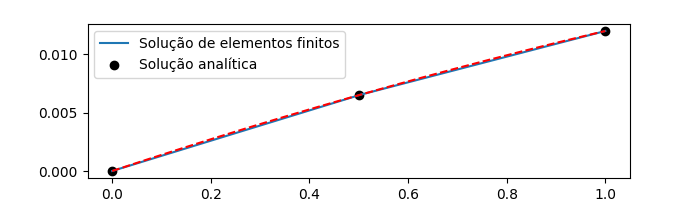
\includegraphics[scale=1]{Figures/4-Elemento_barra/Deslocamento_exemplo_4-1.png}
            \caption{Comparação entre deslocamento analítico e aproximado.}
            \label{fig:exemplo_desl_comp}
        \end{figure}

        Com a expressão do deslocamento, podemos reconstruir algumas outras grandezas associadas a ele. Por exemplo, podemos calcular a deformação aproximada em cada elemento como:

        \begin{equation*}
            \varepsilon^h(x) = \frac{du^h(x)}{dx} = a_1 \frac{d N_1}{dx} + a_2 \frac{d N_2}{dx} + a_3 \frac{d N_3}{dx} 
            = \begin{bmatrix}
            \frac{dN_1}{dx} &
            \frac{dN_2}{dx} &
            \frac{dN_3}{dx}
            \end{bmatrix}
            \begin{Bmatrix}
                a_1\\
                a_2\\
                a_3
            \end{Bmatrix}
            = \mathbf{B}\mathbf{a}
        \end{equation*}

        \begin{equation*}
            \varepsilon^h(x) = 
            \left\{
            \begin{array}{cl}
                0.013 & 0 \leq x \leq 0.5\\
                0.011 & 0.5 \leq x \leq 1\\
                0 & \text{qualquer outro ponto}\\
            \end{array}
            \right.
        \end{equation*}

        Note que, como a função chapéu é linear, a deformação então será constante dentro de cada elemento. Podemos comparar com a solução analítica (Figura \ref{fig:exemplo_def_comp}) dada por:

        \begin{figure}[h!]
            \centering
            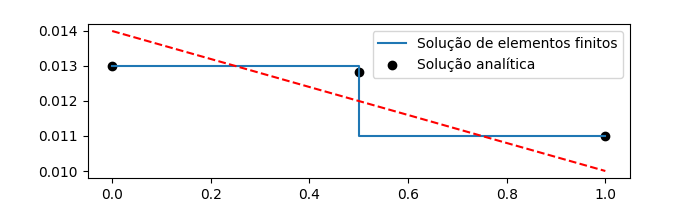
\includegraphics[scale=1]{Figures/4-Elemento_barra/Deformacao_exemplo_4-1.png}
            \caption{Comparação entre deformações analítica e aproximada.}
            \label{fig:exemplo_def_comp}
        \end{figure}

        \begin{equation*}
            \varepsilon(x) = -0.004x + 0.014
        \end{equation*}

        Podemos também comparar as tensões aproximada e analítica (Figura \ref{fig:exemplo_tens_comp}):

        \begin{figure}[h!]
            \centering
            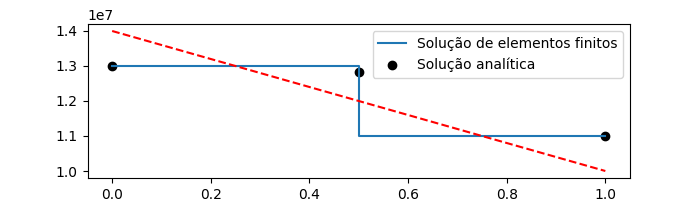
\includegraphics[scale=1]{Figures/4-Elemento_barra/Tensao_exemplo_4-1.png}
            \caption{Comparação entre tensões analítica e aproximada.}
            \label{fig:exemplo_tens_comp}
        \end{figure}

        \begin{equation*}
            \sigma^h(x) = E\varepsilon^h(x) = Ea_1 \frac{d N_1}{dx} + Ea_2 \frac{d N_2}{dx} + Ea_3 \frac{d N_3}{dx} 
            = E\begin{bmatrix}
            \frac{dN_1}{dx} &
            \frac{dN_2}{dx} &
            \frac{dN_3}{dx}
            \end{bmatrix}
            \begin{Bmatrix}
                a_1\\
                a_2\\
                a_3
            \end{Bmatrix}
            = \mathbf{D}\mathbf{B}\mathbf{a}
        \end{equation*}

        \begin{equation*}
            \sigma^h(x) = 
            \left\{
            \begin{array}{cl}
                13 MPa & 0 \leq x \leq 0.5\\
                11 MPa & 0.5 \leq x \leq 1\\
                0 & \text{qualquer outro ponto}\\
            \end{array}
            \right.
        \end{equation*}

        \begin{equation*}
            \sigma(x) = -4x + 14 [MPa]
        \end{equation*}

        Finalmente, podemos verificar a reação de apoio e o esforço normal interno na barra. Para encontrar a reação $R_x$, podemos voltar a equação que descartamos do sistema linear e resolvê-la:

        \begin{equation*}
            R_x = -14 N
        \end{equation*}

        Comparamos então os esforços internos:

        \begin{equation*}
            N_x(0) = \left.EA\frac{du}{dx}\right|_{x=0} = -4x+14 = 14 N
        \end{equation*}

        \begin{equation*}
            N_x(1) = \left.EA\frac{du}{dx}\right|_{x=1} = -4x+14 = 10 N
        \end{equation*}

        \begin{equation*}
            N_x^h(0) = \left.EA\frac{du^h}{dx}\right|_{x=0} = 13N
        \end{equation*}

        \begin{equation*}
            N_x^h(1) = \left.EA\frac{du^h}{dx}\right|_{x=1} = 11 N
        \end{equation*}

        Perceba que, embora a reação de apoio seja igual à reação analítica ($N_x(0)$), a condição de contorno de Neumann imposta não é exata, isto é $N_x^h(L) \neq N_x(L)$.

    \subsection{Matriz elementar}

        O procedimento mostrado anteriormente ainda é bastante trabalhoso. Podemos simplificá-lo, dividindo a integração elemento a elemento. Note que, ao integrarmos no exemplo, já tivemos que dividir o domínio de integração nos elementos. Portanto, podemos já fazer isso logo de início, integrar uma matriz menor para cada elemento, e depois juntá-la numa matriz maior.

        Considere o $e$-ésimo elemento de uma malha de elementos de barra, ele terá as seguintes funções de forma dentro dele:

        \begin{equation}
            N_1(x) = \frac{x_{e+1}-x}{h_e} \rightarrow \frac{dN_1}{dx} = -\frac{1}{h_e}
        \end{equation}

        \begin{equation}
            N_2(x) = \frac{x-x_e}{h_e} \rightarrow \frac{dN_2}{dx} = \frac{1}{h_e}
        \end{equation}

        Uma integração no domínio total da estrutura $\Omega$ pode ser subdividido na soma de integrais no domínio de cada elemento da malha (Figura \ref{fig:dominio_discretizado}):

        \begin{equation}
            \int_{\Omega} f(x) dA = \int_{\Omega_{e_1}} f(x) dA + \int_{\Omega_{e_2}} f(x) dA + \cdots + \int_{\Omega_{e_n}} f(x) dA
        \end{equation}

        \begin{figure}[h!]
            \centering
            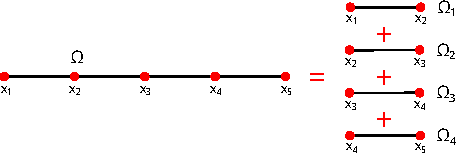
\includegraphics[scale=1.3]{Figures/4-Elemento_barra/Dominio.pdf}
            \caption{Dividindo o intervalo de integração nos vários elementos}
            \label{fig:dominio_discretizado}
        \end{figure}

        Portanto, em vez de montar a matriz do sistema global de uma vez, podemos encontrar uma matriz para cada elemento, avaliando a integral no domínio deste elemento.

        Considerando um elemento de barra $e$:

        

        \begin{equation*}
            \mathbf{K}_e = \int_{x_e}^{x_{e+1}} \mathbf{B}_e^T \mathbf{D}_e\mathbf{B}_e dx = \int_{x_e}^{x_{e+1}} EA 
            \begin{Bmatrix}
            \frac{dN_1}{dx}\\
            \frac{dN_2}{dx}
            \end{Bmatrix}
            \begin{bmatrix}
            \frac{dN_1}{dx} &
            \frac{dN_2}{dx}
            \end{bmatrix} dx
        \end{equation*}

        \begin{equation*}
            \mathbf{K}_e = \int_{x_e}^{x_{e+1}} EA 
            \begin{Bmatrix}
            -\frac{1}{h_e}\\
            \frac{1}{h_e}
            \end{Bmatrix}
            \begin{bmatrix}
            -\frac{1}{h_e} &
            \frac{1}{h_e}
            \end{bmatrix} dx
        \end{equation*}

        \begin{equation*}
            \mathbf{K}_e = \int_{x_e}^{x_{e+1}} \frac{EA}{h_e^2} 
            \begin{Bmatrix}
            -1\\
            1
            \end{Bmatrix}
            \begin{bmatrix}
            -1 &
            1
            \end{bmatrix} dx
        \end{equation*}

        \begin{equation*}
            \mathbf{K}_e = 
            \frac{EA}{h_e^2}\begin{bmatrix}
                1 & -1\\
                -1 & 1
            \end{bmatrix}
            \int_{x_e}^{x_{e+1}} dx
        \end{equation*}

        \begin{equation*}
            \mathbf{K}_e = 
            \frac{EA}{h_e^2}\begin{bmatrix}
                1 & -1\\
                -1 & 1
            \end{bmatrix}
            \left(x_{e+1} - x_e\right)
        \end{equation*}


        \begin{equation}
            \mathbf{K}_e = 
            \frac{EA}{h_e}\begin{bmatrix}
                1 & -1\\
                -1 & 1
            \end{bmatrix}
        \end{equation}

        Similarmente, podemos avaliar a integral da força elemento a elemento. Considere o mesmo elemento de barra com uma força distribuída uniforme $p$.


        \begin{equation*}
            \mathbf{f}_e = \int_{x_e}^{x_{e+1}} 
            \begin{Bmatrix}
            N_1\\
            N_2
            \end{Bmatrix} 
            p dx =
            \int_{x_e}^{x_{e+1}} 
            \begin{Bmatrix}
            \frac{x_{e+1}-x}{h_e}\\
            \frac{x-x_e}{h_e}
            \end{Bmatrix} 
            p dx
        \end{equation*}

        \begin{equation*}
            \mathbf{f}_e = 
            \left. p
            \begin{Bmatrix}
            \frac{2x_{e+1}x-x^2}{2h_e}\\
            \frac{x^2-2x_e x}{2h_e}
            \end{Bmatrix}\right|_{x_e}^{x_{e+1}} =
            p
            \begin{Bmatrix}
            \frac{x_{e+1}^2-2x_{e+1}x_e+x_e^2}{2h_e}\\
            \frac{x_{e+1}^2-2x_{e+1}x_e+x_e^2}{2h_e}
            \end{Bmatrix} = 
            p
            \begin{Bmatrix}
            \frac{\left(x_{e+1}-x_e\right)^2}{2h_e}\\
            \frac{\left(x_{e+1}-x_e\right)^2}{2h_e}
            \end{Bmatrix}
        \end{equation*}

        \begin{equation*}
            \mathbf{f}_e = 
            p
            \begin{Bmatrix}
            \frac{h_e^2}{2h_e}\\
            \frac{h_e^2}{2h_e}
            \end{Bmatrix} = 
            p
            \begin{Bmatrix}
            \frac{h_e}{2}\\
            \frac{h_e}{2}
            \end{Bmatrix}
        \end{equation*}

        \begin{equation*}
            \mathbf{f}_e = \frac{p h_e}{2}
            \begin{Bmatrix}
                1\\
                1 
            \end{Bmatrix}
        \end{equation*}


    \subsection{Montagem do sistema global}

        Um dado elemento $e$ vai ter sua matriz de rigidez $\mathbf{K}_e$ e seu vetor de forças $\mathbf{f}_e$. Este elemento apenas contém uma parte de todas as funções de forma do sistema (no caso da barra, duas), e portanto, essa matriz e esse vetor serão de tamanho bastante inferior ao tamanho da matriz global.

        Considerando o mesmo elemento anterior, o sistema deste elemento, fica $2 \times 2$, da seguinte forma:

        \begin{equation}
            \mathbf{K}_e \mathbf{a}_e = \mathbf{f}_e 
        \end{equation}
        
        \begin{equation}
            \frac{EA}{h_e}\begin{bmatrix}
                1 & -1\\
                -1 & 1
            \end{bmatrix}
            \begin{Bmatrix}
                a_{e}\\
                a_{e+1}\\
            \end{Bmatrix}=
            \begin{Bmatrix}
                f_{e}\\
                f_{e+1}\\
            \end{Bmatrix}
        \end{equation}

        Talvez uma das primeiras coisas que o leitor possa perceber é que o sistema acima não possui solução única. Isso é esperado, visto que um elemento é apenas uma pequena parte do sistema completo e por si só não representa adequadamente o sistema.

        O sistema global, conforme mostrado anteriormente, incluirá todos os graus de liberdade do sistema, inclusive aqueles apenas presentes em outros elementos:

        \begin{equation}
            \begin{bmatrix}
                K_{11} & K_{12} & \cdots & K_{1n}\\
                K_{21} & K_{22} & \cdots & K_{2n}\\
                \vdots & \vdots & \ddots & \vdots\\
                K_{n1} & K_{n2} & \cdots & K_{nn}\\
            \end{bmatrix}
            \begin{Bmatrix}
                a_1\\
                a_2\\
                \vdots\\
                a_n
            \end{Bmatrix}
            =
            \begin{Bmatrix}
                f_1\\
                f_2\\
                \vdots\\
                f_n
            \end{Bmatrix}
        \end{equation}

        Portanto, para obtermos o sistema global, precisamos fazer o procedimento de montagem da matriz de global. A montagem é feita da seguinte forma: verificamos a matriz de rigidez elementar do elemento que estamos analisando. Vemos os deslocamentos deste elemento. Inserimos os termos da matriz elementar na matriz global, nas linhas e colunas correspondentes àquele deslocamento. O procedimento de montagem muitas vezes tem a seguinte notação:

        \begin{equation}
            \mathbf{K} = \assembly_{e=1}^n \mathbf{K}_e
        \end{equation}
 

        Por exemplo, considere uma barra sujeita a uma carga distribuída uniforme, discretizada em dois elementos. O primeiro elemento possui os graus de liberdade $1$ e $2$. O segundo possui os graus de liberdade $2$ e $3$. A montagem da matriz e vetor globais, é feita inserindo esses termos nas posições correspondentes na matriz global, isto é:

        \begin{equation*}
            \mathbf{K} = 
            \begin{bmatrix}
                \frac{EA}{h_1} & -\frac{EA}{h_1} & 0\\
                -\frac{EA}{h_1} & \frac{EA}{h_1} + \frac{EA}{h_2} & -\frac{EA}{h_2}\\
                0 & -\frac{EA}{h_2} & \frac{EA}{h_2}
            \end{bmatrix}
        \end{equation*}

        \begin{equation*}
            \mathbf{f} = 
            \begin{Bmatrix}
                \frac{p h_1}{2}\\
                \frac{p h_1}{2} + \frac{p h_2}{2}\\
                \frac{p h_2}{2}
            \end{Bmatrix}
        \end{equation*}

        Portanto, em vez de resolvermos as integrais no domínio global, montamos as matrizes de rigidez de cada elemento (note que, se os elementos forem idênticos, suas matrizes serão iguais!). Montadas a matriz e vetor globais, nós realizamos o procedimento de montagem.

        Esta abordagem nos permite simplificar as integrais, reduzindo o domínio de integração de uma geometria possivelmente complexa na soma de integrais em geometrias mais simples (como quadrados e triângulos no 2D). Ela também nos permite adicionar tipos diferentes de elementos em locais diferentes do domínio.

        Nas próximas seções, veremos como tratar cada elemento. Como definir as funções de forma em coordenadas locais centradas no próprio elemento de análise, nos permitindo a construção de ``blocos'' para montar a malha, independentemente de onde esse elemento estará.

        \subsubsection*{Propriedades da matriz global}

        Antes de continuar a trabalhar nos elementos e suas funções de forma, vamos salientar algumas propriedades importantes da matriz de rigidez de elementos finitos. Em muitos casos, para simular de forma precisa alguma estrutura, precisamos usar milhões ou até bilhões de elementos finitos. Nestes casos, chegamos à matrizes com possivelmente centenas de milhões ou até bilhões de linhas e colunas. Evidentemente, se a solução de um sistema linear desta magnitude fosse impossível, o MEF não seria um método tão importante na engenharia quanto ele é. Esta seção discutirá algumas propriedades da matriz que torna esse sistema linear viável de resolver.

        A matriz de rigidez elementar (e consequentemente a global), será simétrica e semi-positivo definida. Uma matriz é dita semi-positivo definida quando:

        \begin{equation}
            x^T K x \geq 0, \quad \forall x \in \mathcal{R}^n,
        \end{equation}

        \noindent isto é equivalente a dizer que todos os autovalores da matriz são não negativos (positivos ou nulos).

        Após aplicar as condições de contorno suficientes para tornar o sistema isostático ou hiperestático, a matriz se torna positivo definida. Neste caso, seus autovalores serão estritamente positivos e a desigualdade da expressão acima tem um operador de maior, em vez de maior ou igual. A consequência direta dessa propriedade é que o sistema linear terá apenas uma solução.

        Outra vantagem dessas propriedades da matriz de rigidez está na seleção dos métodos de solução do sistema. A matriz ser simétrica e real permite a utilização da fatoração de Cholesky (similar a fatoração LU, porém com $L = U^T$, utilizando metade da memória e do tempo). A matriz ser positivo-definida permite a aplicação de métodos iterativos na solução do sistema (comuns em casos muito grandes), como o método dos Gradientes Conjugados.

        Entretanto, a propriedade mais importante dessas matrizes, é que elas são esparsas. Uma matriz esparsa é uma matriz cuja grande maioria dos termos é nula. No MEF, a matriz global terá os termos da diagonal principal não nulos. Fora da diagonal principal, serão não nulos apenas termos correspondentes a deslocamentos que compartilham algum elemento. No caso de uma malha com elementos de barra dispostos sequencialmente, cada linha da matriz terá, no máximo, três termos não nulos, mesmo que a matriz tenha milhões de linhas! Similarmente, se temos um elemento quadrado com quatro nós, cada um com deslocamento horizontal e vertical, cada linha da matriz global terá, no máximo, 18 termos não nulos. Note que, além de possuir poucos termos não nulos, o número máximo possível é bastante previsível.

        Na computação, existem duas formas de armazenar matrizes na memória. A primeira e mais usual é armazená-la como uma matriz densa. Uma matriz densa possui todos os seus elementos salvos na memória de forma explícita. Por exemplo, uma matriz 100x100, ocupará um espaço de 10 mil variáveis \textit{float} na memória. Outra forma de salvar uma matriz na memória é como uma matriz esparsa. Existem várias formas de armazenar uma matriz esparsa, mas a mais usual é salvá-la como COO (lista coordenada). Em vez de salvar cada termo, salvam-se apenas os termos não nulos (Figura \ref{fig:matriz_esparsa}). Para isso, para cada um deles, salvam-se três valores: sua linha, sua coluna e seu valor. No exemplo de uma matriz 100x100, considerando 5 termos não nulos por linha, teremos apenas 500 não nulos na matriz inteira. Portanto, precisamos de apenas 1000 variáveis do tipo \textit{int} e 500 do tipo float para armazenar a mesma matriz que necessitaria de 10 mil \textit{floats} para armazenar como densa.

        \begin{figure}[h!]
            \centering
            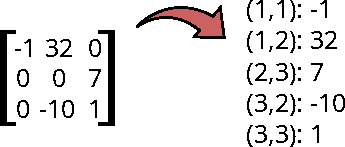
\includegraphics[scale=1]{Figures/4-Elemento_barra/Esparsa.pdf}
            \caption{Representação de uma matriz como uma matriz densa e como uma matriz esparsa do tipo COO.}
            \label{fig:matriz_esparsa}
        \end{figure}

        Por exemplo, considere um problema de MEF 2D de condução de calor com um milhão de elementos. Cada linha, neste caso, terá nove termos não nulos. O número total de linhas na matriz será por volta de um milhão também, então suponhamos que continue com este valor, para simplificar o exemplo. Se armazenássemos essa matriz de forma densa, precisariamos salvar $10^6 \times 10^6 = 10^{12}$ termos do tipo \textit{float}. Supondo que cada variável ocupe 8 \textit{bytes} na memória, precisaríamos de $73$ TB de memória! Nem um disco rígido médio seria capaz de armazenar esta matriz!

        Como uma matriz COO, considerando que as duas variáveis \textit{int} e a variável \textit{float} ocupem o mesmo espaço na memória, teremos apenas $9 \times 3 \times 10^6 = 27 \cdot 10^6$ termos para salvar. Considerando os mesmos 8 \textit{bytes} por termo, reduzimos o espaço na memória para apenas $206$ MB! Reduz-se o custo em memória para um valor que até a memória RAM de um \textit{smartwatch} ou uma calculadora gráfica seria capaz de armazenar!


    \subsection{Coordenadas locais e mudança de coordenadas}

        Na seção anterior, vimos que precisamos calcular apenas as matrizes elementares de cada elemento. Feito esse cálculo, apenas montamos eles para chegarmos na matriz global. Entretanto, a matriz elementar ainda possui limites de integração que dependem da posição do elemento na malha. Para modificar essa integração, tornando-a menos dependente diretamente da posição do elemento, utilizaremos coordenadas locais em cada elemento.

        Considere o elemento na Figura \ref{fig:coord_local_barra}. Definiremos um sistema de coordenadas locais $\xi$. Desta forma, todo elemento de barra será mapeado para este elemento em coordenadas locais. O sistema de coordenadas em coordenadas locais sempre será definido com os limites de $-1$ a $1$, para utilizarmos o procedimento de integração numérica da próxima seção. Portanto, os dois nós do elemento de barra estarão em $\xi_1 = -1$ e $\xi_2 = 1$, para cada elemento.

        \begin{figure}[h!]
            \centering
            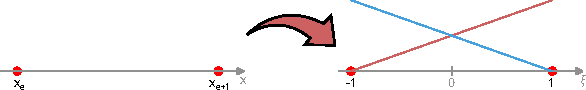
\includegraphics[scale=1.5]{Figures/4-Elemento_barra/Coordenada_local.pdf}
            \caption{Mudança de coordenadas de um elemento de barra de coordenadas globais para coordenadas locais. Funções de forma representadas na coordenada local.}
            \label{fig:coord_local_barra}
        \end{figure}

        Ademais, as funções de forma de cada elemento serão definidas em coordenadas locais. De forma similar a seção anterior, as funções de forma do elemento de barra com dois nós são:

        \begin{equation*}
            N_1(\xi) = \frac{1}{2}\left(1-\xi\right)
       \end{equation*}

       \begin{equation*}
            \frac{dN_1}{d\xi} = -\frac{1}{2}
       \end{equation*}

       \begin{equation*}
            N_2(\xi) = \frac{1}{2}\left(1+\xi\right)
       \end{equation*}

       \begin{equation*}
            \frac{dN_2}{d\xi} = \frac{1}{2}
       \end{equation*}

       Portanto, o deslocamento em um dado elemento é dado por:

       \begin{equation*}
            u^h(\xi) = N_1(\xi) a_1 + N_2(\xi) a_2
       \end{equation*}

       Se considerarmos que o elemento de barra em questão possui como nós os pontos com coordenadas $x_i$ e $x_{i+1}$, podemos definir um mapeamento entre a coordenada global $x$ e a coordenada local $\xi$ pelas funções de forma:

       \begin{equation*}
            x(\xi) = N_1(\xi) x_i + N_2(\xi) x_{i+1}
       \end{equation*}

       A derivada desse mapeamento será importante nas deduções a seguir, portanto vamos escrevê-la aqui:

       \begin{equation*}
            \frac{dx}{d\xi} = \frac{dN_1}{d\xi} x_i + \frac{dN_2}{d\xi} x_{i+1}
       \end{equation*}

       \begin{equation}
            \frac{dx}{d\xi} = \frac{x_{i+1}-x_i}{2} = \frac{h_e}{2}
       \end{equation}

       No caso unidimensional, temos essa expressão da derivada. Em casos 2D ou 3D, teremos um sistema com duas ou três coordenadas, respectivamente, tanto globais quanto locais. A combinação das derivadas das coordenadas globais em relação às locais definira um termo conhecido como \textbf{matriz Jacobiana}. O determinante dessa matriz representa a razão do comprimento/área/volume (a depender se é 1D, 2D ou 3D) entre o elemento em coordenadas globais e locais.

       Também precisaremos do inverso dessa derivada, para isso, usamos a regra da cadeia:

       \begin{equation*}
            \frac{dx}{d\xi} \frac{d\xi}{dx} = \frac{dx}{dx} = 1 
       \end{equation*}

       \begin{equation*}
            \frac{d\xi}{dx} = \left(\frac{dx}{d\xi}\right)^{-1} = \frac{2}{h_e}
       \end{equation*}

       Finalmente, para calcularmos a matriz de rigidez do elemento, precisamos dos termos $\frac{dN_1}{dx}$ e $\frac{dN_2}{dx}$. Note que as derivadas são em relação \textbf{às coordenadas globais, não às locais!} Uma grande fonte de erro é utilizar as derivadas $\frac{dN_1}{d\xi}$ em vez de $\frac{dN_1}{dx}$ na montagem da matriz. Para encontramos a derivada em relação à coordenada global, podemos usar a regra da cadeia, novamente:

       \begin{equation*}
            \frac{dN_1}{dx} = \frac{dN_1}{d\xi} \frac{d\xi}{dx} = -\frac{1}{2} \frac{2}{h_e} = -\frac{1}{h_e}
       \end{equation*}

       \begin{equation*}
            \frac{dN_2}{dx} = \frac{dN_2}{d\xi} \frac{d\xi}{dx} = \frac{1}{2} \frac{2}{h_e} = \frac{1}{h_e}
       \end{equation*}


       \begin{equation*}
            \mathbf{B} = 
            \begin{bmatrix}
            \frac{dN_1}{dx} &
            \frac{dN_2}{dx}
            \end{bmatrix} = 
            \begin{bmatrix}
            -\frac{1}{h_e} &
            \frac{1}{h_e}
            \end{bmatrix}=
            \frac{1}{h_e}
            \begin{bmatrix}
            -1 &
            1
            \end{bmatrix}
       \end{equation*}

       Finalmente, voltamos à integração da matriz elementar:

       \begin{equation*}
            \mathbf{K}_e = \int_{\Omega_e} \mathbf{B}^T \mathbf{D} \mathbf{B} dx
        \end{equation*}

        Do Cálculo, podemos nos lembrar que é possível modificar o domínio de integração por mudança de coordenadas da seguinte forma:

        \begin{equation*}
            \int_{\Omega_x} f(x) dx = \int_{\Omega_y} f(x(y)) \frac{dx}{dy} dy
        \end{equation*}


        Portanto, para o elemento de barra:

        \begin{equation*}
            \mathbf{K}_e = \int_{\Omega_e} \mathbf{B}^T \mathbf{D} \mathbf{B} dx
        \end{equation*}


        \begin{equation*}
            \mathbf{K}_e = \int_{-1}^1 \mathbf{B}^T \mathbf{D} \mathbf{B} \frac{dx}{d\xi} d\xi
        \end{equation*}


        \begin{equation*}
            \mathbf{K}_e = \int_{-1}^1 \frac{EA}{h_e^2}
            \begin{Bmatrix}
            -1 \\
            1
            \end{Bmatrix}
            \begin{bmatrix}
            -1 &
            1
            \end{bmatrix} \frac{h_e}{2} d\xi
        \end{equation*}

        \begin{equation*}
            \mathbf{K}_e =  \frac{EA}{2h_e}
            \begin{bmatrix}
             1 & -1\\
            -1 &  1
            \end{bmatrix} \int_{-1}^1 d\xi
        \end{equation*}

        \begin{equation*}
            \mathbf{K}_e = 
            \frac{EA}{h_e}
            \begin{bmatrix}
                1 & -1 \\
                -1 & 1 \\
            \end{bmatrix}
        \end{equation*}

        Chegamos ao mesmo resultado que o anterior. Embora possa parecer trivial para o caso da barra, mostraremos como isso pode simplificar ao modificar as funções de forma na seção seguinte.

        A mesma coisa pode ser feita para o vetor de forças:

        \begin{equation*}
            f_{1} = \int_{\Omega_e} N_1(x) p(x) dx = \int_{-1}^1 N_1(\xi) p(\xi) \frac{dx}{d\xi} d\xi
        \end{equation*}

        \begin{equation*}
            f_{2} = \int_{\Omega_e} N_2(x) p(x) dx = \int_{-1}^1 N_2(\xi) p(\xi) \frac{dx}{d\xi} d\xi
        \end{equation*}

    \subsection{Polinômios de Lagrange}
    \label{sec:lagrange}

        Já passamos toda a formulação do elemento em coordenadas locais, mantendo apenas o termo de transformação da variável de integração e da regra da cadeia das derivadas internas. Desta forma, temos agora a liberdade de modificar as funções de forma do elemento.

        De forma geral, as funções de forma são polinomiais. Mais especificamente, no MEF, são utilizados os polinômios de Lagrange. Os polinômios de Lagrange são um conjunto de $n+1$ polinômios de grau $n$ que interpolam $n+1$ pontos, de forma que apenas um deles é não nulo em cada ponto. Isto é, para definir um conjunto de polinômios de Lagrange de grau $n$, seguimos o procedimento:

        
        \begin{enumerate}
            \item Dados $n+1$ pontos $\left\{x_0, x_1, \cdots, x_n\right\}$;
            \item Os $n+1$ polinômios de Lagrange de ordem $n$ $\left\{l_0(x), l_1(x), \cdots, l_n(x)\right\}$ são aqueles que têm a propriedade:
            
            \begin{equation*}
                \begin{array}{cccc}
                    l_0(x_0) = 1 & l_0(x_1) = 0 & \cdots & l_0(x_n) = 0\\
                    l_1(x_0) = 0 & l_1(x_1) = 1 & \cdots & l_1(x_n) = 0\\
                    \vdots & \vdots & \ddots & \vdots\\
                    l_n(x_0) = 0 & l_n(x_1) = 0 & \cdots & l_n(x_n) = 1\\
                \end{array}
            \end{equation*}
        \end{enumerate}

        A grande consequência desta propriedade dos polinômios de Lagrange, é que, dada uma função definida pela composição desses polinômios:

        \begin{equation}
            f(x) = \sum\limits_{i=1}^{n+1} l_i(x) a_i,
        \end{equation}

        Em cada um dos pontos definidos, o valor da função será exatamente o coeficiente correspondente ao polinômio de Lagrange que é não nulo naquele ponto:

        \begin{equation}
            f(x_i) = a_i.
        \end{equation}

        Portanto, no contexto de elementos finitos, em que cada um desses pontos serão nós da malha, o deslocamento nos nós serão exatamente os termos do vetor de deslocamento nodal:

        \begin{equation}
            u(\xi_i) = \sum\limits_{i=1}^{n+1} l_i(\xi_i) a_i = a_i 
        \end{equation}

        Perceba que, até o momento, \textbf{já estamos utilizando o par de polinômios de Lagrange de grau 1!} Portanto, precisamos apenas saber como montar elementos de ordem superior, sendo a ordem do elemento definida como o grau das suas funções de forma.

        \subsubsection*{Exemplo: grau 1}

        \begin{equation*}
                \xi_0 = -1, \quad \xi_1 = 1
            \end{equation*}

        \begin{equation*}
            \begin{array}{cc}
                N_1(-1) = 1 & N_1(1) = 0\\
                N_2(-1) = 0 & N_2(1) = 1
            \end{array}
        \end{equation*}

        \begin{equation*}
            N_1(\xi) = a_0 + b_0 \xi
        \end{equation*}

        \begin{equation*}
            1 = a_0 - b_0, \quad 0 = a_0 + b_0
        \end{equation*}

        \begin{equation*}
            a_0 = \frac{1}{2}, \quad b_0 = -\frac{1}{2}
        \end{equation*}

        \begin{equation*}
            N_1(\xi) = \frac{1}{2}\left(1-\xi\right)
        \end{equation*}

        \begin{equation*}
            N_2(\xi) = \frac{1}{2}\left(1+\xi\right)
        \end{equation*}

        \subsubsection*{Exemplo: grau 2}

        \begin{equation*}
                \xi_0 = -1, \quad \xi_1 = 0 , \quad \xi_2 = 1
            \end{equation*}

        \begin{equation*}
            \begin{array}{ccc}
                N_1(-1) = 1 & N_1(0) = 0 & N_1(1) = 0\\
                N_2(-1) = 0 & N_2(0) = 1 & N_2(1) = 0\\
                N_3(-1) = 0 & N_3(0) = 0 & N_3(1) = 1\\
            \end{array}
        \end{equation*}

        \begin{equation*}
            N_1(\xi) = a_0 + b_0 \xi + c_0 \xi^2
        \end{equation*}

        \begin{equation*}
            1 = a_0 - b_0 + c_0, \quad 0 = a_0 , \quad 0 = a_0 + b_0 + c_0
        \end{equation*}

        \begin{equation*}
            a_0 = 0, \quad b_0 = -\frac{1}{2} , \quad c_0 = \frac{1}{2}
        \end{equation*}

        \begin{equation*}
            N_1(\xi) = \frac{\xi}{2}\left(\xi-1\right) \rightarrow \frac{dN_1}{d\xi} = \xi-\frac{1}{2}
        \end{equation*}

        \begin{equation*}
            N_2(\xi) = 1-\xi^2 \rightarrow \frac{dN_2}{d\xi} = -2\xi
        \end{equation*}

        \begin{equation*}
            N_3(\xi) = \frac{\xi}{2}\left(\xi+1\right) \rightarrow \frac{dN_3}{d\xi} = \xi+\frac{1}{2}
        \end{equation*}

        \begin{equation*}
            x(\xi) = N_1(\xi) x_i + N_2(\xi) x_{i+1} + N_3(\xi) x_{i+2}
        \end{equation*}

       \begin{equation*}
            \frac{dx}{d\xi} = \frac{dN_1}{d\xi} x_i + \frac{dN_2}{d\xi} x_{i+1} + \frac{dN_3}{d\xi} x_{i+2}
       \end{equation*}

       \begin{equation*}
            \frac{dx}{d\xi} = \left(\xi-\frac{1}{2}\right) x_i - 2\xi x_{i+1} + \left(\xi+\frac{1}{2}\right) x_{i+2}
       \end{equation*}

       \begin{equation*}
            \frac{dx}{d\xi} = \xi \left(x_i - 2x_{i+1} + x_{i+2}\right) + \frac{x_{i+2}-x_i}{2}
       \end{equation*}

       Se considerarmos que $x_{i+1}$ está no meio dos outros dois pontos $\left(x_{i+1} = \frac{x_{i+2}+x_i}{2}\right)$:

       \begin{equation*}
            \frac{dx}{d\xi} =\frac{h_e}{2}
       \end{equation*}

       \begin{equation*}
            \frac{d\xi}{dx} =\frac{2}{h_e}
       \end{equation*}

       \begin{equation*}
            \frac{dN_1}{dx} = \frac{dN_1}{d\xi} \frac{d\xi}{dx}  = \frac{1}{h_e}\left(2\xi-1\right)
        \end{equation*}

        \begin{equation*}
            \frac{dN_2}{dx} = \frac{dN_2}{d\xi} \frac{d\xi}{dx} = -\frac{4\xi}{h_e}
        \end{equation*}

        \begin{equation*}
            \frac{dN_3}{dx} = \frac{dN_3}{d\xi} \frac{d\xi}{dx} = \frac{1}{h_e}\left(2\xi+1\right)
        \end{equation*}

        \begin{equation*}
            \mathbf{K}_e = \int_{-1}^{1} \mathbf{B}^T\mathbf{D}\mathbf{B} \frac{dx}{d\xi} d\xi
        \end{equation*}

        \begin{equation*}
            \mathbf{K}_e = \int_{-1}^{1} EA 
            \begin{Bmatrix}
            \frac{dN_1}{dx}\\
            \frac{dN_2}{dx}\\
            \frac{dN_3}{dx}\\
            \end{Bmatrix}
            \begin{bmatrix}
            \frac{dN_1}{dx} &
            \frac{dN_2}{dx} &
            \frac{dN_3}{dx}
            \end{bmatrix} \frac{dx}{d\xi} d\xi
        \end{equation*}


        \begin{equation*}
            \mathbf{K}_e = 
            \frac{EA}{3h_e}
            \begin{bmatrix}
                7 & -8 & 1 \\
                -8 & 16 & -8 \\
                1 & -8 & 7
            \end{bmatrix}
        \end{equation*}


        \subsubsection*{Forma geral de definir o polinômio de Lagrange de grau $n$}

        \begin{equation*}
            l_j(x) = \frac{x-x_0}{x_j-x_0} \cdots \frac{x-x_{j-1}}{x_j-x_{j-1}} \frac{x-x_{j+1}}{x_j-x_{j+1}} \cdots \frac{x-x_n}{x_j-x_n}
        \end{equation*}

        \begin{equation*}
            l_j(x) = \prod_{\underset{k \neq j}{0\leq k \leq n}} \frac{x-x_k}{x_j-x_k}
        \end{equation*}

    \subsection{Integração por Quadratura de Gauss-Legendre}
    \label{sec:integracao1D}

        Finalmente, possuimos todos os blocos necessários para construir um programa adequado de elementos finitos. Apenas nos carece um detalhe sobre o procedimento: como realizar a integração nos elementos?

        Em alguns casos, como nos elementos de barra, é possível escrever analíticamente a expressão da integral e obter expressões fechadas para a matriz de rigidez. Neste caso, podemos apenas pegar diretamente essa matriz obtida analiticamnte e empregá-la na montagem do sistema. global. Entretanto, em elementos mais complexos, ou mesmo na integração de forças descritas por funções complexas, nem sempre é possível ou viável integrar analíticamente. Portanto, esta seção se empenhará em introduzir o método de integração numérica aplicado em elementos finitos: a integração por quadratura de Gauss-Legendre.

        Antes de falar sobre a integração em si, é necessário definir outro tipo de polinômio, os polinômios de Legendre.



        \subsubsection{Polinômios de Legendre}

        Suponha o espaço vetorial dos polinômios de grau menor ou igual a $n$, $\mathcal{P}_n(\mathbb{R})$. Este espaço terá dimensão $n$, podemos escrever uma base como, por exemplo, os monômios de cada grau. Por exemplo, um polinômio $p(x)$ pode ser escrito em função de uma base de $p_0(x)$, $p_1(x)$, $\cdots$, $p_n(x)$. Por exemplo:

        \begin{equation}
            p(x) = 4x^2 + 3x - 2 = 4p_2(x) + 3p_1(x) - 2p_0(x)
        \end{equation}

        No espaço de funções, podemos definir o produto interno através de uma integral. No caso, podemos definir um produto interno entre dois polinômios $p(x)$ e $q(x)$ como:

        \begin{equation}
            \int_{-1}^1 p(x) q(x) dx
        \end{equation}

        O polinômio de Legendre de grau $n$ é definido como o polinômio que, dado o produto interno acima, é ortogonal a todos os polinômios de grau inferior, isto é:

        \begin{equation}
            \int_{-1}^{1} P_n(x) p(x) = 0, \quad 0\leq dim(p(x)) <n
        \end{equation}

        Ele também tem a propriedade de $P_n(1) = 1$.

        Visto que o $P_n(x)$ é ortogonal a todos os polinômios de grau inferior, então ele será ortogonal a todos os polinômios de Legendre de grau inferior. Portanto, o conjunto $\left\{P_0(x), P_1(x), \cdots, P_n(x)\right\}$ formam uma base de $\mathcal{P}_n$.

        Do teorema fundamental da álgebra, o polinômio de grau $n$ deve possuir $n$ raízes. Consequentemente, ele também pode ser fatorado da seguinte forma:

        \begin{equation}
            P_n(x) = C \prod_{j=1}^n \left(x-x_j\right)
        \end{equation}

        Consequentemente, sua derivada também pode ser escrita como:

        \begin{equation}
            P_n'(x) = C \sum_{k=1}^n \left[\prod_{\underset{j \neq k}{j=1}}^n \left(x-x_j\right)\right]
        \end{equation}

        \begin{equation}
            P_n'(x_i) = C \prod_{\underset{j \neq i}{j=1}}^n \left(x_i-x_j\right)
        \end{equation}

        Um conjunto de polinômios de Lagrange também podem ser escritos em função dos polinômios de Legendre:

        \begin{equation}
            l_i(x) = \frac{P_n(x)}{\left(x-x_i\right)P_n'(x_i)} = 
            \frac{C \prod_{j=1}^n \left(x-x_j\right)}{\left(x-x_i\right)C \prod_{\underset{j \neq k}{j=1}}^n \left(x_i-x_j\right)}
        \end{equation}

        \begin{equation}
            l_i(x) =
            \frac{\prod_{\underset{j \neq k}{j=1}}^n \left(x-x_j\right)}{\prod_{\underset{j \neq i}{j=1}}^n \left(x_i-x_j\right)}
        \end{equation}

        Note que para cada $x=x_j$ com $j\neq i$, haverá algum fator nulo no numerador, que zerá a função. Se $x=x_i$, o numerador fica igual ao denominador e a função assume valor unitário.
    

        \subsubsection*{Exemplo: grau 0}

        \begin{equation*}
            P_0(x) = 1
        \end{equation*}

        \subsubsection*{Exemplo: grau 1}

        \begin{equation*}
            P_1(x) = a_1x + a_0
        \end{equation*}

        \begin{equation*}
            \int_{-1}^{1} P_1(x) P_0(x) = 0
        \end{equation*}

        \begin{equation*}
            \int_{-1}^{1} \left( a_1x + a_0\right) 1 = 0
        \end{equation*}

        \begin{equation*}
            \left[ \frac{a_1}{2}x^2 + a_0 x\right]_{-1}^1 = 0
        \end{equation*}

        \begin{equation*}
            a_0 = 0
        \end{equation*}

        \begin{equation*}
            P_1(1) = a_1 x = 1
        \end{equation*}

        \begin{equation*}
            a_1= 1
        \end{equation*}

        \begin{equation*}
            P_1(x) = x 
        \end{equation*}


        \subsubsection*{Exemplo: grau 2}

        \begin{equation*}
            P_2(x) = b_2x^2 + b_1 x + b_0
        \end{equation*}

        \begin{equation*}
            \int_{-1}^{1} \left(b_2x^2 + b_1 x + b_0\right) x = 0
        \end{equation*}

        \begin{equation*}
            \left[ \frac{b_2}{4}x^4 + \frac{b_1}{3}x^3 + \frac{b_0}{2}x^2\right]_{-1}^1 = 0
        \end{equation*}

        \begin{equation*}
            b_1= 0
        \end{equation*}


        \begin{equation*}
            \int_{-1}^{1} \left(b_2x^2 + b_0\right) 1 = 0
        \end{equation*}

        \begin{equation*}
            \left[ \frac{b_2}{3}x^3 + b_0 x\right]_{-1}^1 = 0
        \end{equation*}

        \begin{equation*}
            b_2 + 3b_0= 0
        \end{equation*}


        \begin{equation*}
            P_2(1) = b_2x^2 + b_0 = 1
        \end{equation*}

        \begin{equation*}
            b_2 + b_0= 0
        \end{equation*}

        \begin{equation*}
            b_2= \frac{3}{2}
        \end{equation*}

        \begin{equation*}
            b_0= -\frac{1}{2}
        \end{equation*}

        \begin{equation*}
            P_2(x) = \frac{3}{2}x^2 - \frac{1}{2}
        \end{equation*}


        \subsubsection{Quadratura de Gauss-Legendre}

        Agora podemos abordar diretamente o tópico da integração numérica. De forma geral, temos uma integral do seguinte tipo:
        
        \begin{equation}
            \int_{-1}^{1} f(\xi) d\xi
        \end{equation}

        No contexto de elementos finitos, note que sempre chegamos a uma integral deste tipo ao utilizar o procedimento de mudança de coordenadas:

        \begin{equation}
            \int_{\Omega_e} h(x) dx = \int_{-1}^{1} h(x(\xi)) \frac{dx}{d\xi} d\xi = \int_{-1}^{1} f(\xi) d\xi
        \end{equation}

        Desejamos aproximar a integral por poucos retângulos, aproximadas em pontos específicos e com retângulos de larguras específicas, a tornar a integral o mais exata possível com o mínimo de pontos possível:

        \begin{equation}
            \int_{-1}^{1} f(\xi) d\xi \approx \sum_{i=1}^n f(\xi_i) w_i
        \end{equation}

        O procedimento de integração será baseado em encontrar o melhor conjunto de $n$ pontos $\xi_i$ e seus respectivos pesos $w_i$ tais que a integral é mais exata possível. Para encontrar esses pontos, podemos usar as \textbf{raízes do polinômio de Legendre de grau n.}

        Considere então uma função $f(\xi)$ de grau menor ou igual a $n$. Ela pode ser escrita como uma combinação linear dos polinômios de Lagrange formado pelas raízes do polinômio de Legendre de grau $n$:

        \begin{equation}
            f(\xi) = \sum_{i=1}^n a_i l_i(\xi) = \sum_{i=1}^n f(\xi_i) l_i(\xi)
        \end{equation}

        \noindent no qual a segunda igualdade vem diretamente da propriedade dos polinômios de Lagrange.

        Portanto, a integral fica:

        \begin{equation}
            \int_{-1}^{1} f(\xi) d\xi = \int_{-1}^{1} \sum_{i=1}^n f(\xi_i) l_i(\xi) d\xi =  \sum_{i=1}^n f(\xi_i) \int_{-1}^{1} l_i(\xi) d\xi
        \end{equation}

        Portanto, já encontramos uma expressão \textbf{exata} para integrar um polinômio de grau $n$ com apenas $n$ pontos de integração para avaliar, o peso é o termo da integral do polinômio de Lagrange:

        \begin{equation}
            w_i = \int_{-1}^{1} l_i(\xi) d\xi = \int_{-1}^{1} \frac{P_n(\xi)}{\left(\xi-\xi_i\right)P_n'(\xi_i)} d\xi
        \end{equation}

        Empregando algumas propriedades do polinômio de Legendre, chegamos à seguinte expressão:

        \begin{equation}
            w_i = \frac{2}{\left(1-\xi_i^2\right)\left(P_n'(\xi_i)\right)^2}
        \end{equation}

        Usualmente, é comum tabelar os pontos e os pesos em função do grau $n$, em vez de resolver explicitamente as raízes de $P_n(\xi)$ para obter os $\xi_i$ e integrar para obter os $w_i$. A Tabela \ref{tab:gauss} mostra alguns pares de pontos e pesos para alguns valores de $n$.

        \begin{table}[h!]
        \centering
        \caption{Pontos e pesos variando o grau.}
        \label{tab:gauss}
        \begin{tabular}{|c|c|c|}
            \hline
            $n$  & $\xi_i$ & $w_i$ \\ \hline
            $1$ & $0$ & $2$ \\ \hline
            $2$ & $-\frac{1}{\sqrt{3}}$, $\frac{1}{\sqrt{3}}$ & $1$, $1$ \\ \hline
            $3$ & $-\sqrt{0.6}$, $0$ ,$\sqrt{0.6}$ & $\frac{5}{9}$, $\frac{8}{9}$, $\frac{5}{9}$ \\ \hline
        \end{tabular}
    \end{table}

        \subsubsection*{Verificação do erro}

        Considere agora um polinômio $f(\xi)$ de grau $P$. Se usarmos $N$ pontos de Gauss, teremos o polinômio de Legendre de grau $N$. Podemos dividir $f(\xi)$ por este polinômio:

        \begin{equation}
            f(\xi) = q(\xi) P_N(\xi) + r(\xi)
        \end{equation}

        \noindent no qual, o quociente $q(\xi)$ e o resto $r(\xi)$ deverão ter um grau menor ou igual a $P-N$.

        Se avaliarmos essa função nos pontos de Gauss, e lembrando que estes são raízes de $P_N(\xi)$, obtemos:

        \begin{equation}
            f(\xi_i) = q(\xi_i)P_N(\xi_i) + r(\xi_i) = r(\xi_i)
        \end{equation}

        Além disso, a integral de $f(\xi)$ fica:

        \begin{equation}
            \int_{-1}^{1} f(\xi) d\xi = \int_{-1}^{1} q(\xi)P_N(\xi) d\xi + \int_{-1}^{1} r(\xi) d\xi
        \end{equation}

        Pela propriedade dos polinômios de Legendre, se $q(\xi)$ tiver grau inferior a $P_N(\xi)$, então a primeira integral deve se anular. Isto é, se $P-N < N$, então:

        \begin{equation}
            \int_{-1}^{1} q(\xi)P_N(\xi) d\xi = 0
        \end{equation}

        Portanto:

        \begin{equation}
            \int_{-1}^{1} f(\xi) d\xi = \int_{-1}^{1} r(\xi) d\xi
        \end{equation}

        Como $r(\xi)$ é um polinômio de grau $P-N$, e já adotamos a hipótese que isso deve ser menor que $N$. Então a quadratura com $N$ pontos deve ser exata. Isto é, utilizando as relações anteriores:

        \begin{equation}
            \int_{-1}^{1} f(\xi) d\xi = \int_{-1}^{1} r(\xi) d\xi = \sum_{i=1}^n r(\xi_i) w_i = \sum_{i=1}^n f(\xi_i) w_i 
        \end{equation}


        Portanto, a integração de um polinômio de grau $P$ será exata se usarmos $N$ pontos de Gauss, respeitando a seguinte expressão:

        \begin{equation}
            N \geq \frac{P+1}{2}
        \end{equation}

        \subsubsection{Exemplo 1}

        Resolva a integral abaixo usando integração de Gauss-Legendre:

         \begin{equation*}
            \int_{0}^{1} sen(x) dx
        \end{equation*}

        \subsubsection*{Solução}

        A solução analítica desta derivada é da seguinte forma:

        \begin{equation*}
            \int_{0}^{1} sen(x) dx = -\left.cos(x)\right|_0^1 = -cos(1)+cos(0) \approx 0.4597
        \end{equation*}

        Para resolver por Gauss-Legendre, precisamos primeiro mudar o sistema de coordenadas para outro tal que os limites de integração sejam $-1$ e $1$. Um sistema de coordenadas linear que faz isso é:

        \begin{equation*}
            x(\xi) = \frac{1}{2}\left(1+\xi\right)
        \end{equation*}

        \begin{equation*}
            \frac{dx}{d\xi} = \frac{1}{2}
        \end{equation*}

        Portanto, podemos mudar o sistema de coordenadas da integral:

        \begin{equation*}
            \int_{0}^{1} sen(x) dx = \int_{-1}^{1} sen\left[\frac{1}{2}\left(1+\xi\right)\right] \frac{1}{2} d\xi
        \end{equation*}

        Usando a quadratura de Gauss, integramos para $n$ pontos, usando $f(\xi) = sen\left[\frac{1}{2}\left(1+\xi\right)\right] \frac{1}{2}$. Como a função seno não é polinomial, nunca teremos garantia da exatidão da integral, não importa quantos pontos adotarmos.

        \begin{equation*}
            n = 1 \rightarrow \int_{0}^{1} sen(x) dx \approx 0.4794 \rightarrow \text{erro de } 4,29\% 
        \end{equation*}

        \begin{equation*}
            n = 2 \rightarrow \int_{0}^{1} sen(x) dx \approx 0.4596 \rightarrow \text{erro de } 0,024\% 
        \end{equation*}

        \begin{equation*}
            n = 3 \rightarrow \int_{0}^{1} sen(x) dx \approx 0.4597 \rightarrow \text{erro de } 5,13 \cdot 10^{-5}\% 
        \end{equation*}

        Entretanto, note que o erro cai rapidamente quando aumentamos o número de pontos. 


        \subsubsection{Exemplo 2}

        Resolva a integral abaixo usando integração de Gauss-Legendre:

         \begin{equation*}
            \int_{2}^{4} 5x^4 dx
        \end{equation*}

        \subsubsection*{Solução}

        Novamente, podemos resolvê-la analiticamente:

        \begin{equation*}
            \int_{2}^{4} 5x^4 dx = \left.x^5\right|_{2}^4 = 4^5 - 2^5 = 1024 - 32 = 992 
        \end{equation*}

        Transformando para um sistema de coordenadas cujos limites de integração são $-1$ e $1$:

        \begin{equation*}
            x(\xi) = 3+\xi
        \end{equation*}

        \begin{equation*}
            \frac{dx}{d\xi} = 1
        \end{equation*}

        Portanto, a integral fica:

        \begin{equation*}
            \int_{2}^{4} 5x^4 dx = \int_{-1}^{1} 5\left(3+\xi\right)^4 d\xi
        \end{equation*}


        Note que esta integral é um polinômio de grau $P=4$ em $\xi$. Portanto, podemos encontrar um número mínimo de pontos de Gauss tal que esta integral é exata:

        \begin{equation*}
            N \geq \frac{P+1}{2} = \frac{4+1}{2} = 2,5
        \end{equation*}

        Como é impossível pegar ``meio'' ponto, então a integral deve ser exata a partir de $3$ pontos. Resolvemos para alguns pontos a seguir:

        \begin{equation*}
            n = 1 \rightarrow \int_{2}^{4} 5x^4 dx \approx 810 \rightarrow \text{erro de } 18,35\% 
        \end{equation*}

        \begin{equation*}
            n = 2 \rightarrow \int_{2}^{4} 5x^4 dx \approx 991,11 \rightarrow \text{erro de } 0,090\% 
        \end{equation*}

        \begin{equation*}
            n = 3 \rightarrow \int_{2}^{4} 5x^4 dx = 992 \rightarrow \text{erro de } 0\% 
        \end{equation*}

        A integral fica exata para $n=3$. Se a calculássemos para $n$ maiores, ainda obteríamos a integral exata.


\subsection{Conclusão}

    Nesta seção, verificamos como funciona o MEF para um elemento de barra. As ferramentas estudadas aqui já são suficientes para resolver qualquer problema, envolvendo qualquer física e qualquer geometria. Evidentemente, alguns ajustes devem ser feitos, seja nas funções de forma usadas, seja no método de integração, seja em outros aspectos. Desta forma, o procedimento geral é o seguinte:

    \begin{enumerate}
        \item Verificar qual a equação diferencial do problema;
        \item Aplicar o método dos resíduos ponderados e Galerkin, para obter a forma fraca da aproximação desta equação;
        \item Discretizar o domínio de análise em elementos finitos, estes que provêm de um mapeamento com um elemento em coordenadas locais. Este elemento em coordenadas locais deve ser definido pelas suas funções de forma;
        \item Utilizando as funções de forma e as relações entre coordenadas locais e globais, obter a expressão da matriz de rigidez e vetor de forças do sistema;
        \item Integrar a matriz de rigidez e o vetor de forças de cada elemento, usando um método de integração por quadratura;
        \item Montar a matriz global do sistema a partir das elementares;
        \item Resolver o sistema linear;
        \item Reconstruir o deslocamento/tensão/deformação a partir dos deslocamentos nodais e das funções de forma dos elementos.
    \end{enumerate}

    Muitas dessas etapas são realizadas a priori, por quem estiver programando o método. De forma geral, um programa de elementos finitos se empenha nas seguintes etapas:

    \begin{enumerate}
        \item Discretização do domínio (gerador de malha);
        \item Integrar a matriz de rigidez e o vetor de forças de cada elemento;
        \item Montar a matriz global do sistema a partir das elementares;
        \item Resolver o sistema linear;
        \item Reconstruir o deslocamento/tensão/deformação a partir dos deslocamentos nodais e das funções de forma dos elementos.
    \end{enumerate}


	%LTeX: language=pt-br
% !TeX root = Apostila_IM381.tex

\cleardoublepage
\section{Revisão modelo de viga}

    Nesta seção, será apresentada uma revisão do modelo de barra, sua equação diferencial, com alguns exemplos e exercícios.

    \subsection{Hipóteses}

        As principais hipóteses do modelo de barra são:

        \begin{itemize}
            \item Estrutura esbelta - comprimento muito maior que sua largura ou espessura;
            \item Material linear elástico isotrópico;
            \item Pequenas deformações e pequenos deslocamentos;
            \item Submetido apenas a forças transversais ou momentos fletores;
            \item Deformações locais desprezíveis (princípio de Saint-Venant).
            \item Seção plana permanece plana após a deformação
        \end{itemize}

    \subsection{Dedução da equação diferencial}

        Considere a viga com uma seção transversal variável, sujeita a forças $q(x)$ (Figura \ref{fig:viga}). Um elemento infinitesimal (Figura \ref{fig:infinitesimal_viga}) dessa viga também deve estar em equilíbrio.

        \begin{figure}[h!]
            \centering
            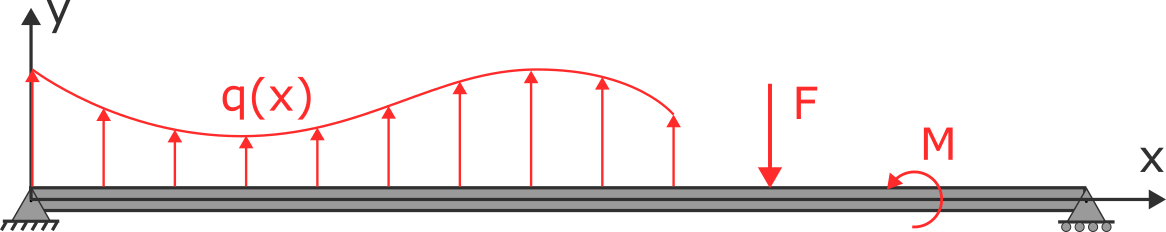
\includegraphics[scale=1]{Figures/5-Viga/Cargas.png}
            \caption{Viga sujeita a esforços externos}
            \label{fig:viga}
        \end{figure}

        \begin{figure}[h!]
            \centering
            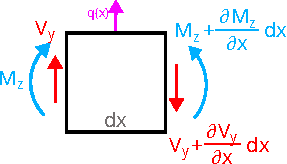
\includegraphics[scale=1.5]{Figures/5-Viga/Infinitesimal.pdf}
            \caption{Elemento infinitesimal de uma viga}
            \label{fig:infinitesimal_viga}
        \end{figure}

        \begin{equation*}
            \sum F_y = 0
        \end{equation*}

        \begin{equation*}
            q(x)dx + V_y - \left(V_y + \frac{dV_y}{dx}dx\right) = 0
        \end{equation*}

        \begin{equation}
            \frac{dV_y}{dx} = q(x)
            \label{eq:viga_dv}
        \end{equation}

        \begin{equation*}
            \sum M_z = 0
        \end{equation*}

        \begin{equation*}
            -V_y\frac{dx}{2} - \left(V_y + \frac{dV_y}{dx}dx\right)\frac{dx}{2} - M_z + \left(M_z + \frac{dM_z}{dx}dx\right) = 0
        \end{equation*}

        \begin{equation*}
            \frac{dM_z}{dx} = V_y + q(x)\frac{dx}{2}
        \end{equation*}

        \begin{equation}
            \frac{dM_z}{dx} = V_y
            \label{eq:viga_dm}
        \end{equation}

        \noindent no qual $M_z(x)$ é chamado momento fletor e $V_y(x)$ é o esforço cortante. Estes são os esforços internos que surgem na estrutura.

        As Eq. \eqref{eq:viga_dv} e Eq. \eqref{eq:viga_dm} representam o equilíbrio do sistema. Podemos juntá-la em:

        \begin{equation}
            \frac{d^2M_z}{dx^2} = q(x)
            \label{eq:viga_equilibrio}
        \end{equation}

        Para a cinemática da viga, consideremos a viga da Figura \ref{fig:deslocamento_viga}, com uma deflexão $v(x)$ e ângulo $\theta(x)$. O modelo mais simples de viga se chama modelo de Euler-Bernoulli. Neste modelo, a deformação devido ao cisalhamento da viga é desprezado. Por exemplo, se pegarmos um livro e dobrarmos, vemos que as folhas dele vão se atritar umas nas outras. No modelo de Euler-Bernoulli, consideramos que as folhas estão todas coladas entre si.

        \begin{figure}[h!]
            \centering
            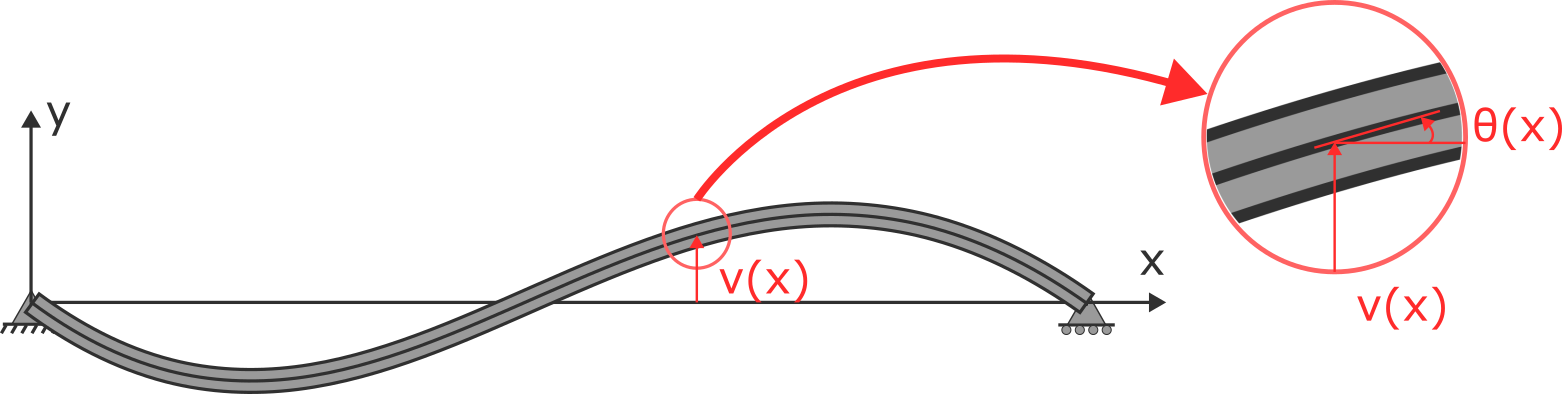
\includegraphics[scale=0.8]{Figures/5-Viga/Deslocado.png}
            \caption{Viga deslocada devido a esforços externos}
            \label{fig:deslocamento_viga}
        \end{figure}

        Considere o elemento infinitesimal não deformado e o deformado (Figura \ref{fig:viga_deform_infinitesimal}). Uma das hipóteses deste modelo, que se verifica na prática, é que suas superfícies planas permanecerão planas, isto é, os lados desse elemento permanecerão retos. O elemento se deformará, formando um arco de disco. Haverá uma linha transversal ao longo do elemento na qual o comprimento deste elemento não altera. Esta linha se chama linha neutra. O raio da circunferência descrita pela linha neutra neste elemento infinitesimal é o raio de curvatura $\rho(x)$.

        \begin{figure}[h!]
            \centering
            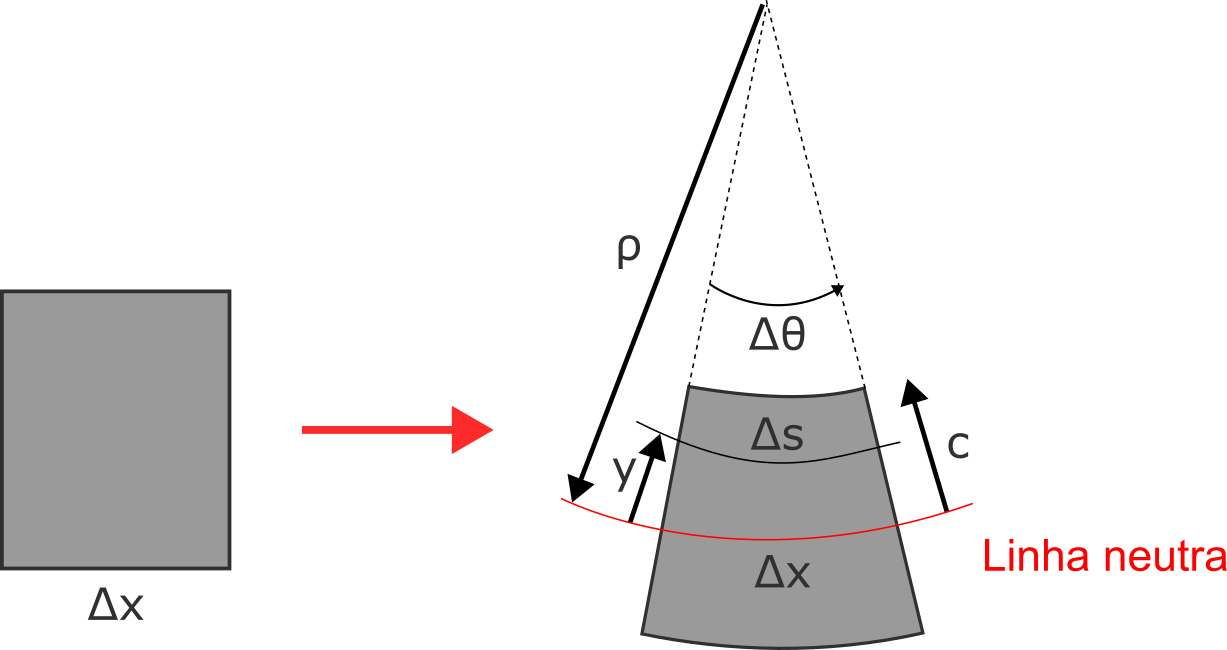
\includegraphics[scale=0.8]{Figures/5-Viga/Cinematica.png}
            \caption{Deformação de um elemento infinitesimal de viga}
            \label{fig:viga_deform_infinitesimal}
        \end{figure}

        A deformação normal ao longo desse elemento é calculada pela variação dos comprimentos desse elemento:

        \begin{equation*}
            \varepsilon_{xx}(x,y) = \lim_{\Delta x \rightarrow 0} \frac{\Delta s - \Delta x}{\Delta x}
        \end{equation*}

        \begin{equation}
            \varepsilon_{xx}(x,y) = -\frac{y}{\rho(x)}
        \end{equation}

        Portanto, a deformação segue um perfil linear, como na Figura \ref{fig:viga_deformacao}. Consequentemente, pela lei de Hooke ($\sigma_{xx} = E \varepsilon_{xx}$), temos que a tensão também será linear (Figura \ref{fig:viga_tensao}):

        \begin{figure}[h!]
            \begin{subfigure}{0.49\textwidth}
                \centering
                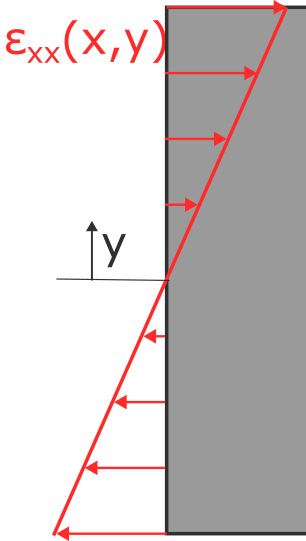
\includegraphics[scale=0.8]{Figures/5-Viga/Deformacao.png}
                \caption{}
                \label{fig:viga_deformacao}
            \end{subfigure}
            ~
            \begin{subfigure}{0.49\textwidth}
                \centering
                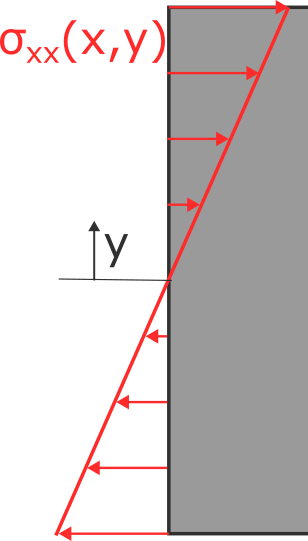
\includegraphics[scale=0.8]{Figures/5-Viga/Tensao.png}
                \caption{}
                \label{fig:viga_tensao}
            \end{subfigure}
            \caption{Tensão e deformação de viga ao longo da seção transversal. (a) Deformação, (b) tensão.}
        \end{figure}


        \begin{equation}
            \sigma_{xx}(x,y) = -\frac{Ey}{\rho(x)}
        \end{equation}

        Considere agora a seção da Figura \ref{fig:equilibrio_secao_viga}. A força resultante, devido a essas tensões, deve ser igual nula, pois não há forças axiais:

        \begin{figure}[h!]
            \centering
            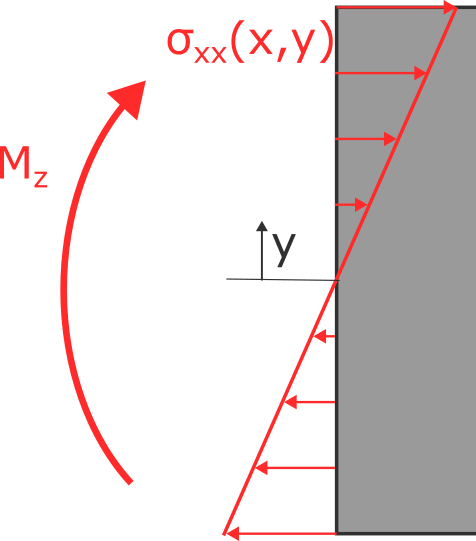
\includegraphics[scale=0.8]{Figures/5-Viga/Momento_res.png}
            \caption{Equilíbrio de forças na seção da viga}
            \label{fig:equilibrio_secao_viga}
        \end{figure}

        \begin{equation*}
            F_x = \int_A \sigma_{xx} dA = 0
        \end{equation*}

        \begin{equation*}
            F_x = -\frac{E}{\rho(x)} \int_A y dA = 0
        \end{equation*}

        \noindent a integral de área é pela área da seção transversal, que é função de $y$ e $z$, portanto, o termo $\rho(x)$ é constante e pode ser movido para fora.

        A expressão $\int_A y dA$ é o primeiro momento de área. Ela pode ser usada para encontrar a posição da linha neutra na estrutura. O resultado obtido aqui indica que a linha neutra deve passar pelo centroide da seção transversal.

        Da mesma forma, o momento resultante deve ser igual ao momento fletor (se atente aos sinais da expressão, conforme a regra da mão direita):

        \begin{equation*}
            -M_z - \int_A y \sigma_{xx} dA = 0
        \end{equation*}

        \begin{equation*}
            M_z = \frac{E}{\rho(x)} \int_A y^2 dA = \frac{EI_{zz}}{\rho}
        \end{equation*}

        \noindent no qual $I_{zz}$ será o momento de inércia da seção transversal em relação ao eixo z que passa pelo seu centroide.

        \begin{equation}
            \frac{1}{\rho} = \frac{M_z}{EI_{zz}}
        \end{equation}

        \begin{equation}
            \sigma_{xx}(x,y) = -\frac{M_z}{I_{zz}}y
        \end{equation}

        A tensão, na viga, portanto, deve ser máxima nas extremidades da seção transversal e onde se encontram os maiores valores de momento fletor.

        Finalmente, precisamos correlacionar as deflexões e o ângulo de inclinação com o raio de curvatura. Para isso, considere novamente a viga da Figura \ref{fig:deslocamento_viga}. Considerando pequenas deformações e deslocamentos, com ângulos pequenos de inclinação:

        \begin{equation}
            \frac{dv}{dx} = \theta(x)
            \label{eq:viga_defl}
        \end{equation}

        \begin{equation}
            \frac{d\theta}{dx} = \frac{1}{\rho}
            \label{eq:viga_angulo}
        \end{equation}


        Finalmente, juntando Eq. \eqref{eq:viga_equilibrio}, a Eq. \eqref{eq:viga_angulo} e Eq. \eqref{eq:viga_defl}:

        \begin{equation}
            \frac{d^2}{dx^2}\left(EI_{zz}\frac{d^2v}{dx^2}\right) = q(x)
        \end{equation}

        Considerando que a viga tem seção transversal constante e material uniforme:

        \begin{equation}
            EI_{zz}\frac{d^4v}{dx^4} = q(x)
        \end{equation}

        Para obtermos as outras grandezas, podemos integrar sucessivamente:

        \begin{equation}
            \theta(x) = \frac{dv}{dx}
        \end{equation}

        \begin{equation}
            M_z(x) = EI_{zz}\frac{d\theta}{dx} = EI_{zz}\frac{d^2v}{dx^2}
        \end{equation}

        \begin{equation}
            V_y(x) = \frac{dM_z}{dx} = EI_{zz}\frac{d^2\theta}{dx^2} = EI_{zz}\frac{d^3v}{dx^3}
        \end{equation}


    \subsection{Funções de sigularidade}

        Para resolver esta equação diferencial, usamos novamente as funções de singularidade. Neste caso, no entanto, usamos também a função $\left\langle x-a\right\rangle^{-2}$, a derivada do delta de Dirac. Esta é utilizada para representar binários aplicados na viga. A Figura \ref{fig:singularidade_viga} mostra algumas funções de singularidade, incluindo esta.

        \begin{figure}[h!]
            \centering
            
\includegraphics[scale=1.4]{Figures/5-Viga/Singularidade.pdf}
            \caption{Funções de singularidade usadas para a solução da equação da viga}
            \label{fig:singularidade_viga}
        \end{figure}

        A próxima seção mostrará alguns exemplos de solução de vigas usando essas funções.

    \subsection{Exemplo}

        Encontre o deslocamento, rotação, momento fletor e esforço cortante da viga da Figura \ref{fig:viga_exemplo_analit} usando funções de singularidade. Considere $EI_{zz} = 10^3$ Nm$^2$.

        \begin{figure}[h!]
            \centering
            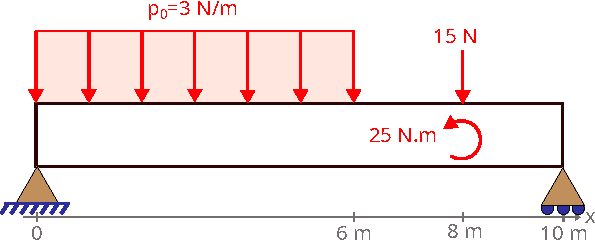
\includegraphics[scale=1]{Figures/5-Viga/Exemplo.pdf}
            \caption{Viga a ser resolvida no exemplo}
            \label{fig:viga_exemplo_analit}
        \end{figure}

        \subsubsection*{Solução}

        A força pode ser escrita como:

        \begin{equation*}
            q(x) = -3 + 3\sing{x}{6}{0} - 15\sing{x}{8}{-1} - 25\sing{x}{8}{-2}
        \end{equation*}


        As condições de contorno são: deslocamento fixo em ambas as extremidades $v(0) = v(10) = 0$ e rotação livre nas extremidades $M_z(0) = M_z(10) = 0$. Portanto:

        \begin{equation*}
            \left\{
            \begin{array}{l}
                EI_{zz}\frac{d^4v}{dx^4} = -3 + 3\sing{x}{6}{0} - 15\sing{x}{8}{-1} - 25\sing{x}{8}{-2}\\
                v(0) = 0\\
                v(10) = 0\\
                M_z(0) = EI_{zz}v''(0) = 0\\
                M_z(10) = EI_{zz}v''(10) = 0
            \end{array}
            \right.
        \end{equation*}

        Para resolver, integramos sucessivamente:

        \begin{equation*}
            V_y(x) = EI_{zz}v'''(x) = -3x + 3\sing{x}{6}{1} - 15\sing{x}{8}{0} - 25\sing{x}{8}{-1} + C_1
        \end{equation*}

        \begin{equation*}
            M_z(x) = EI_{zz}v''(x) = -\frac{3}{2}x^2 + \frac{3}{2}\sing{x}{6}{2} - 15\sing{x}{8}{1} - 25\sing{x}{8}{0} + C_1 x + C_2
        \end{equation*}

        Já podemos aplicar duas condições de contorno:

        \begin{equation*}
            M_z(0) = 0 \rightarrow C_2 = 0
        \end{equation*}

        \begin{equation*}
            M_z(10) = 0 \rightarrow -\frac{3}{2}10^2 + \frac{3}{2}\sing{10}{6}{2} - 15\sing{10}{8}{1} - 25\sing{10}{8}{0} + 10 C_1 = 0
        \end{equation*}

        \begin{equation*}
            C_1 = 18.1 Nm
        \end{equation*}

        Portanto:

        \begin{equation*}
            M_z(x) = EI_{zz}v''(x) = -\frac{3}{2}x^2 + \frac{3}{2}\sing{x}{6}{2} - 15\sing{x}{8}{1} - 25\sing{x}{8}{0} + 18.1 x
        \end{equation*}

        Continuando a integração:

        \begin{equation*}
            EI_{zz}v'(x) = EI_{zz}\theta(x)= -\frac{1}{2}x^3 + \frac{1}{2}\sing{x}{6}{3} - \frac{15}{2}\sing{x}{8}{2} - 25\sing{x}{8}{1} + \frac{18.1}{2} x^2 + C_3
        \end{equation*}

        \begin{equation*}
            EI_{zz}v(x) = -\frac{1}{8}x^4 + \frac{1}{8}\sing{x}{6}{4} - \frac{5}{2}\sing{x}{8}{3} - \frac{25}{2}\sing{x}{8}{2} + \frac{18.1}{6} x^3 + C_3 x + C_4
        \end{equation*}

        Aplicando as outras duas condições de contorno:

        \begin{equation*}
            v(0) = 0 \rightarrow C_4 = 0
        \end{equation*}

        \begin{equation*}
            v(10) = 0 \rightarrow -\frac{1}{8}10^4 + \frac{1}{8}\sing{10}{6}{4} - \frac{5}{2}\sing{10}{8}{3} - \frac{25}{2}\sing{10}{8}{2} + \frac{18.1}{6} 10^3 + 10C_3 = 0
        \end{equation*}

        \begin{equation*}
            C_3 = -17.387 Nm
        \end{equation*}

        O deslocamento, portanto, é:

        \begin{equation*}
            v(x) = \frac{1}{EI_{zz}}\left[-\frac{1}{8}x^4 + \frac{1}{8}\sing{x}{6}{4} - \frac{5}{2}\sing{x}{8}{3} - \frac{25}{2}\sing{x}{8}{2} + \frac{18.1}{6} x^3 - 17.387 x \right] [m]
        \end{equation*}

        \begin{equation*}
            v(x) = -\frac{1}{8}x^4 + \frac{1}{8}\sing{x}{6}{4} - \frac{5}{2}\sing{x}{8}{3} - \frac{25}{2}\sing{x}{8}{2} + \frac{18.1}{6} x^3 - 17.387 x [mm]
        \end{equation*}


        Integrando sucessivamente para voltar às outras grandezas:

        \begin{equation*}
            \theta(x) = \frac{1}{10^3}\left[-\frac{1}{2}x^3 + \frac{1}{2}\sing{x}{6}{3} - \frac{15}{2}\sing{x}{8}{2} - 25\sing{x}{8}{1} + \frac{18.1}{2} x^2 - 17.387\right] [rad]
        \end{equation*}

        \begin{equation*}
            M_z(x) = -\frac{3}{2}x^2 + \frac{3}{2}\sing{x}{6}{2} - 15\sing{x}{8}{1} - 25\sing{x}{8}{0} + 18.1 x [Nm]
        \end{equation*}

        \begin{equation*}
            V_y(x) = -3x + 3\sing{x}{6}{1} - 15\sing{x}{8}{0} + 18.1 [N]
        \end{equation*}

        \noindent note que as funções de singularidade com expoente menor que zero somem das expressões (visto que são funções nulas em qualquer ponto, exceto na singularidade).

        As funções acima são plotadas na Figura \ref{fig:viga_ex_curvas}.

        \begin{figure}
            \begin{subfigure}{0.99\textwidth}
                \centering
                
\includegraphics[scale=0.7]{Figures/5-Viga/deslocamento_ex1.png}
                \caption{}
            \end{subfigure}\\
            \begin{subfigure}{0.99\textwidth}
                \centering
                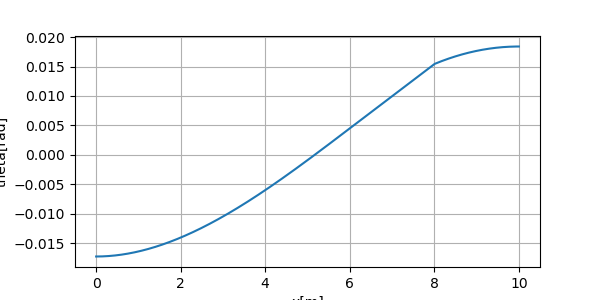
\includegraphics[scale=0.7]{Figures/5-Viga/angulo_ex1.png}
                \caption{}
            \end{subfigure}\\
            \begin{subfigure}{0.99\textwidth}
                \centering
                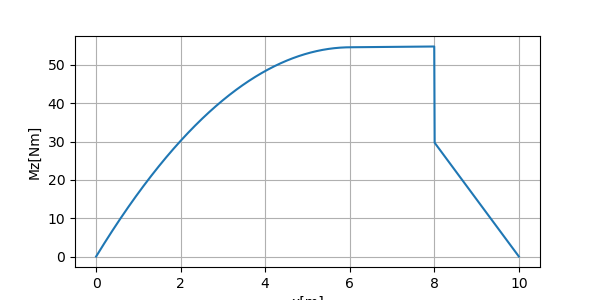
\includegraphics[scale=0.7]{Figures/5-Viga/fletor_ex1.png}
                \caption{}
            \end{subfigure}\\
            \begin{subfigure}{0.99\textwidth}
                \centering
                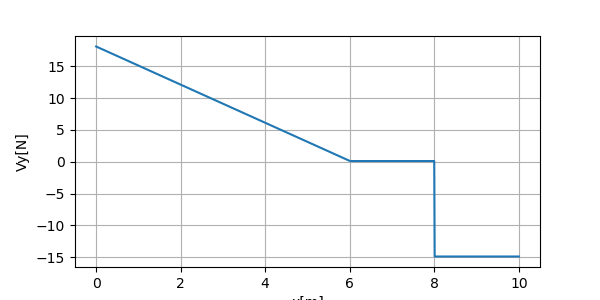
\includegraphics[scale=0.7]{Figures/5-Viga/cortante_ex1.png}
                \caption{}
            \end{subfigure}\\
            \caption{Curvas da viga do Exemplo. (a) Deflexão, (b) rotação, (c) momento fletor e (d) esforço cortante.}
            \label{fig:viga_ex_curvas}
        \end{figure}



	%LTeX: language=pt-br
% !TeX root = Apostila_IM381.tex

\cleardoublepage
\section{Elemento de viga}

    \subsection{Obtenção da forma fraca}

        Conforme visto na seção anterior, a equação diferencial do modelo de viga é:

        \begin{equation}
            EI_{zz}\frac{d^4v}{dx^4} = q(x).
        \end{equation}

        O procedimento a ser utilizado aqui para a aproximação é similar. Sabendo que a solução dessa equação se encontra com $v \in V$, propõe-se a utilização de uma função peso $w \in W$:

        \begin{equation}
            \int_0^L w EI_{zz}\frac{d^4v}{dx^4} dx - \int_0^L w q(x) dx = 0
        \end{equation}

       Da mesma forma como na barra, podemos aplicar integração por partes para chegar à forma fraca do problema de viga. Neste caso, entretanto, como estamos numa equação diferencial de ordem $4$, aplicaremos a integração por parte duas vezes:

        \begin{equation*}
            \int_0^L w EI_{zz}\frac{d^4v}{dx^4} dx = -\int_0^L \frac{dw}{dx} EI_{zz}\frac{d^3v}{dx^3} dx + \left[w EI_{zz}\frac{d^3v}{dx^3}\right]_0^L = -\int_0^L \frac{dw}{dx} EI_{zz}\frac{d^3v}{dx^3} dx + \left[w V_y\right]_0^L
        \end{equation*}

        \begin{equation}
            = \int_0^L \frac{d^2w}{dx^2} EI_{zz}\frac{d^2v}{dx^2} dx + \left[w V_y\right]_0^L - \left[\frac{dw}{dx} EI_{zz}\frac{d^2v}{dx^2}\right]_0^L = \int_0^L \frac{d^2w}{dx^2} EI_{zz}\frac{d^2v}{dx^2} dx + \left[w V_y\right]_0^L - \left[\frac{dw}{dx} M_z\right]_0^L
        \end{equation}

        Portanto, a equação final fica:

        \begin{equation}
            \int_0^L \frac{d^2w}{dx^2} EI_{zz}\frac{d^2v}{dx^2} dx = 
            -w(L) V_y(L) + w(0) V_y(0) + \theta_w(L)M_z(L) - \theta_w(0)M_z(0)+ \int_0^L w q(x) dx
        \end{equation}

        \noindent no qual $\theta_w = \frac{dw}{dx}$.


    \subsection{Polinômios de Hermite}

        No caso da viga, temos duas variáveis que devemos obter em cada ponto do domínio, sendo elas o deslocamento $v(x)$ e a rotação $\theta(x)$. Estas variáveis, no entanto, não são independentes entre si. Conforme mostrado na seção anterior, considerando pequenos deslocamentos e deformações, temos a relação entre elas:

        \begin{equation}
            \theta(x) = \frac{dv}{dx}
        \end{equation}

        Considere um elemento de viga da Figura \ref{fig:malha_viga}. No caso da viga, definem-se normalmente as coordenadas locais $\bar{x}$ como indo de 0 ao comprimento do elemento $h_e$ (Note que $\frac{dx}{d\bar{x}} = 1$). Em cada nó do elemento, há dois graus de liberdade, correspondentes às duas variáveis. O deslocamento e a rotação ao longo do elemento é interpolado pelas funções de forma:

        \begin{figure}[h!]
            \centering
            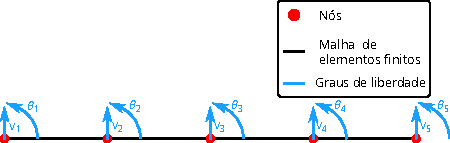
\includegraphics[scale=1.4]{Figures/6-Elemento_viga/Malha_Viga.pdf}
            \caption{Malha com elementos de vigas e seus graus de liberdade.}
            \label{fig:malha_viga}
        \end{figure}

        \begin{equation}
            v(\bar{x}) = \sum\limits_{i=1}^4 N_i(\bar{x}) a_i
        \end{equation}

        \begin{equation}
            \theta(\bar{x}) = \frac{dv}{dx} = \sum\limits_{i=1}^4 N_i'(\bar{x}) a_i
        \end{equation}

        Como há variáveis em $N_i(x)$ e em $N_i(x)$, para obtermos a mesma propriedade de que os coeficientes sejam correspondentes aos deslocamentos nodais, não utilizaremos os polinômios de Lagrange, mas uma outra família de polinômios, chamados \textbf{Polinômios de Hermite}.

        Os polinômios de Hermite são quatro polinômios de grau 3 com as seguintes propriedades:

        \begin{equation*}
            \begin{array}{cccc}
                N_1(\bar{x}_1) = 1, & N_1'(\bar{x}_1) = 0, & N_1(\bar{x}_2) = 0, & N_1'(\bar{x}_2) = 0\\
                N_2(\bar{x}_1) = 0, & N_2'(\bar{x}_1) = 1, & N_2(\bar{x}_2) = 0, & N_2'(\bar{x}_2) = 0\\
                N_3(\bar{x}_1) = 0, & N_3'(\bar{x}_1) = 0, & N_3(\bar{x}_2) = 1, & N_3'(\bar{x}_2) = 0\\
                N_4(\bar{x}_1) = 0, & N_4'(\bar{x}_1) = 0, & N_4(\bar{x}_2) = 0, & N_4'(\bar{x}_2) = 1
            \end{array}
        \end{equation*}

        De forma que tenhamos:

        \begin{equation*}
            \begin{array}{cccc}
                a_1 = v_1, & a_2 = \theta_1, & a_3 = v_2, & a_4 = \theta_2
            \end{array}
        \end{equation*}

        Os polinômios que resolvem este problema são:

        \begin{equation*}
            N_1(\bar{x}) = 2 \left(\frac{\bar{x}}{h_e}\right)^3 - 3 \left(\frac{\bar{x}}{h_e}\right)^2 + 1
        \end{equation*}

        \begin{equation*}
            N_2(\bar{x}) = h_e \left[ \left(\frac{\bar{x}}{h_e}\right)^3 - 2 \left(\frac{\bar{x}}{h_e}\right)^2 + \left(\frac{\bar{x}}{h_e}\right) \right]
        \end{equation*}

        \begin{equation*}
            N_3(\bar{x}) = -2 \left(\frac{\bar{x}}{h_e}\right)^3 + 3 \left(\frac{\bar{x}}{h_e}\right)^2
        \end{equation*}

        \begin{equation*}
            N_4(\bar{x}) = h_e \left[ \left(\frac{\bar{x}}{h_e}\right)^3 - \left(\frac{\bar{x}}{h_e}\right)^2 \right]
        \end{equation*}

        Suas derivadas são:

        \begin{equation*}
            N_1'(\bar{x}) = \frac{1}{h_e} \left[6 \left(\frac{\bar{x}}{h_e}\right)^2 - 6 \left(\frac{\bar{x}}{h_e}\right)\right] \rightarrow N_1''(\bar{x}) = \frac{1}{h_e^2} \left[12 \left(\frac{\bar{x}}{h_e}\right) - 6 \right]
        \end{equation*}

        \begin{equation*}
            N_2'(\bar{x}) = \left[ 3\left(\frac{\bar{x}}{h_e}\right)^2 - 4 \left(\frac{\bar{x}}{h_e}\right) + 1 \right]
            \rightarrow N_2''(\bar{x}) = \frac{1}{h_e} \left[6 \left(\frac{\bar{x}}{h_e}\right) -4 \right]
        \end{equation*}

        \begin{equation*}
            N_3'(\bar{x}) = \frac{1}{h_e} \left[-6 \left(\frac{\bar{x}}{h_e}\right)^2 + 6 \left(\frac{\bar{x}}{h_e}\right)\right] \rightarrow N_3''(\bar{x}) = \frac{1}{h_e^2} \left[-12 \left(\frac{\bar{x}}{h_e}\right) +6 \right]
        \end{equation*}

        \begin{equation*}
            N_4'(\bar{x}) = \left[ 3\left(\frac{\bar{x}}{h_e}\right)^2 - 2\left(\frac{\bar{x}}{h_e}\right) \right] \rightarrow N_4''(\bar{x}) = \frac{1}{h_e} \left[6 \left(\frac{\bar{x}}{h_e}\right) - 2 \right]
        \end{equation*}

        A Figura \ref{fig:hermite} mostra os polinômios de Hermite e suas derivadas avaliadas em um elemento com comprimento $h_e = 1$.

        \begin{figure}[h!]
            \begin{subfigure}{0.99\textwidth}
                \centering
                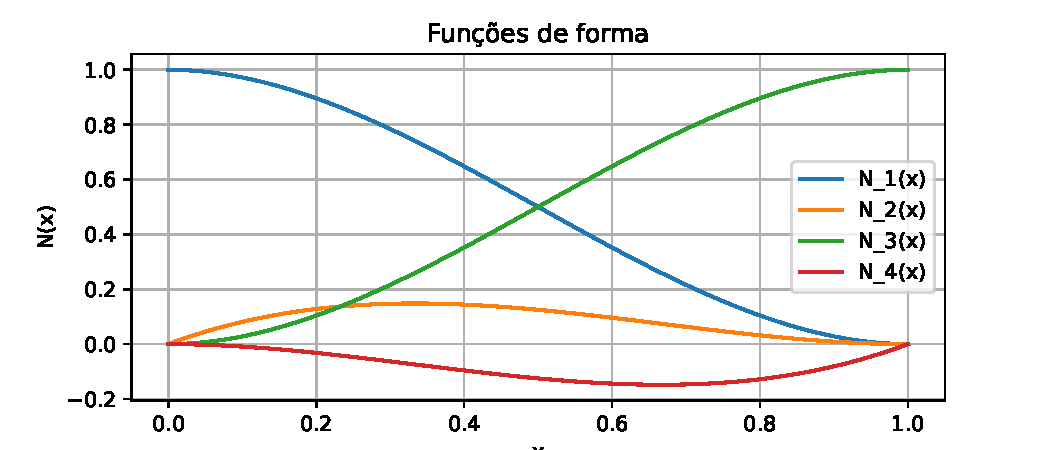
\includegraphics[scale=1]{Figures/6-Elemento_viga/Hermite.pdf}
                \caption{}
            \end{subfigure}
            \\
            \begin{subfigure}{0.99\textwidth}
                \centering
                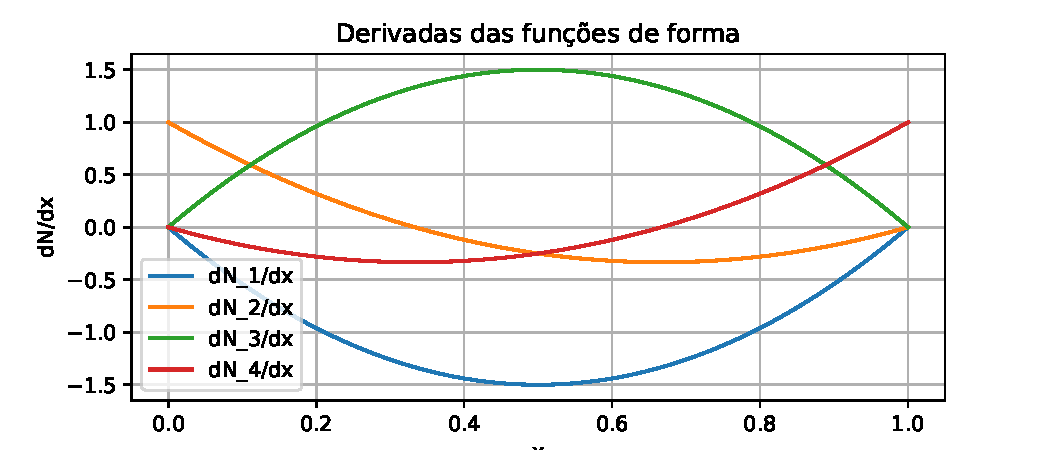
\includegraphics[scale=1]{Figures/6-Elemento_viga/Hermite_deriv.pdf}
                \caption{}
            \end{subfigure}
            \caption{Polinômios de Hermite usados na interpolação de elementos de viga. (a) polinômios de Hermite, (b) derivadas dos polinômios}
            \label{fig:hermite}
        \end{figure}

    \subsection{Resíduos ponderados e Galerkin}

        Com as funções de forma, podemos voltar à forma fraca. Na verdade, podemos definir uma solução aproximada com $v^h(x) \in V^h \subset V$, definida pelas funções de forma provenientes dos polinômios de Hermite. Com o método de Galerkin, as funções peso devem ser provenientes das mesmas funções de forma. Isto é:

        \begin{equation}
            v(\bar{x}) = N_1(\bar{x}) v_1 + N_2(\bar{x}) \theta_1 + N_3(\bar{x}) v_2 + N_4(\bar{x}) \theta_2 = 
            \begin{bmatrix}
                N_1 &
                N_2 &
                N_3 &
                N_4
            \end{bmatrix} 
            \begin{Bmatrix}
                v_1 \\
                \theta_1 \\
                v_2 \\
                \theta_2
            \end{Bmatrix}= 
            \mathbf{N} \mathbf{a}
        \end{equation}

        \begin{equation}
            \theta(\bar{x}) = N_1'(\bar{x}) v_1 + N_2'(\bar{x}) \theta_1 + N_3'(\bar{x}) v_2 + N_4'(\bar{x}) \theta_2 = 
            \frac{d\mathbf{N}}{dx} \mathbf{a}
        \end{equation}

        \begin{equation}
            w(\bar{x}) = N_1(\bar{x}) b_1 + N_2(\bar{x}) b_2 + N_3(\bar{x}) b_3 + N_4(\bar{x}) b_4 = 
            \mathbf{N} \mathbf{b}
        \end{equation}

        \begin{equation}
            \theta_w(\bar{x}) = N_1'(\bar{x}) b_1 + N_2'(\bar{x}) b_2 + N_3'(\bar{x}) b_3 + N_4'(\bar{x}) b_4 = 
            \frac{d\mathbf{N}}{dx} \mathbf{b}
        \end{equation}

        Substituindo essas expressões na forma fraca aproximada:

        
        \begin{equation*}
            \int_0^L \mathbf{b}^T \left(\frac{d^2\mathbf{N}^T}{dx^2} EI_{zz}\frac{d^2\mathbf{N}}{dx^2}\right)\mathbf{a} dx = 
        \end{equation*}

        \begin{equation}
            -\mathbf{b}^T \mathbf{N}(L)^T V_y(L) + \mathbf{b}^T \mathbf{N}(0)^T V_y(0) + \mathbf{b}^T \left.\frac{d\mathbf{N}^T}{dx}\right|_{x=L}M_z(L) - \mathbf{b}^T \left.\frac{d\mathbf{N}^T}{dx}\right|_{x=0}M_z(0)+ \int_0^L \mathbf{b}^T \mathbf{N}(x) q(x) dx
        \end{equation}

        Novamente, como a solução deve ser verificada para qualquer função $w(x)$, então ela deve valer para qualquer $b$. Portanto, devemos resolver o seguinte sistema linear:

        \begin{equation*}
            \left(\int_0^L \frac{d^2\mathbf{N}^T}{dx^2} EI_{zz}\frac{d^2\mathbf{N}}{dx^2} dx \right)\mathbf{a} = 
        \end{equation*}

        \begin{equation}
            -\mathbf{N}(L)^T V_y(L) + \mathbf{N}(0)^T V_y(0) + \left.\frac{d\mathbf{N}^T}{dx}\right|_{x=L}M_z(L) - \left.\frac{d\mathbf{N}^T}{dx}\right|_{x=0}M_z(0)+ \int_0^L \mathbf{N}(x) q(x) dx
        \end{equation}
        
    \subsection{Matriz elementar}

        Dado um elemento, a matriz de rigidez elementar será dada pelos quatro graus de liberdade do elemento:

        \begin{equation*}
            \mathbf{K}_e = \int_0^{h_e} \frac{d^2\mathbf{N}^T}{dx^2} EI_{zz}\frac{d^2\mathbf{N}}{dx^2} d\bar{x}
        \end{equation*}

        \begin{equation}
            \mathbf{K}_e = \int_0^{h_e} 
            \begin{Bmatrix}
                N_1'' \\
                N_2'' \\
                N_3'' \\
                N_4''
            \end{Bmatrix} 
             EI_{zz} 
             \begin{bmatrix}
                N_1'' &
                N_2'' &
                N_3'' &
                N_4''
            \end{bmatrix}  d\bar{x} =
            \int_0^{h_e}
            \mathbf{B}_e^T
            \mathbf{D}_e
            \mathbf{B}_e
            dx
        \end{equation}

        Se substituirmos os polinômios de Hermite e integrarmos, podemos obter matriz de rigidez deste elemento analiticamente:

        \begin{equation}
            \mathbf{K}_e = 
            \frac{EI_{zz}}{h_e^3}
            \begin{bmatrix}
                12   & 6h_e   & -12   & 6h_e   \\
                6h_e & 4h_e^2 & -6h_e & 2h_e^2 \\
                -12  & -6h_e  & 12    & -6h_e  \\
                6h_e & 2h_e^2 & -6h_e & 4h_e^2
            \end{bmatrix}
        \end{equation}


        Podemos fazer o mesmo para o vetor de forças. Integrando-a da seguinte forma:

        \begin{equation}
            \mathbf{f}_e = 
            \int_0^{h_e} 
            \begin{Bmatrix}
                N_1(\bar{x})\\
                N_2(\bar{x})\\
                N_3(\bar{x})\\
                N_4(\bar{x})
            \end{Bmatrix}
            q(x)
            dx
        \end{equation}

        Se considerarmos uma força distribuída uniforma $q_0$ vertical para cima:

        \begin{equation}
            \mathbf{f}_e = 
            \frac{q_0 h_e}{2}
            \begin{Bmatrix}
                1\\
                \frac{h_e}{6}\\
                1\\
                -\frac{h_e}{6}
            \end{Bmatrix}
        \end{equation}


    \subsection{Exemplo}

        Considere a viga da Figura \ref{fig:viga_exemplo_fem}. Assuma $EI_{zz} = 10^3 Nm^2$ e $L=10 m$.

        \begin{figure}[h!]
            \centering
            
\includegraphics[scale=1]{Figures/6-Elemento_viga/Exemplo.pdf}
            \caption{Viga a ser resolvida no exemplo de elementos finitos}
            \label{fig:viga_exemplo_fem}
        \end{figure}

        A solução analítica para essa viga é dada por:

        \begin{equation*}
            u_\text{an}(x) = \frac{1}{EI_{zz}} \left[-\frac{x^5}{120} + \frac{L^2}{12} x^3 - \frac{L^3}{6} x^2\right]
        \end{equation*}

        \begin{equation*}
            \theta_\text{an}(x) = \frac{1}{EI_{zz}} \left[-\frac{x^4}{24} + \frac{L^2}{4} x^2 - \frac{L^3}{3} x\right]
        \end{equation*}

        \begin{equation*}
            {V_y}_\text{an}(x) = -\frac{x^3}{6} + \frac{L^2}{2} x - \frac{L^3}{3}
        \end{equation*}

        \begin{equation*}
            {M_z}_\text{an}(x) = -\frac{x^2}{2} + \frac{L^2}{2}
        \end{equation*}

        Resolvendo por elementos finitos, com dois elementos, há seis graus de liberdade, dois para cada nó. O programa exemplo\_viga.py mostra resolve este problema por elementos finitos usando a biblioteca da disciplina. A Figura \ref{fig:exemplo_viga_mef} mostra o deslocamento, rotação, momento fletor e esforço cortante por elementos finitos e analíticos.

        \begin{figure}[h!]
            \begin{subfigure}{0.46\textwidth}
                \centering
                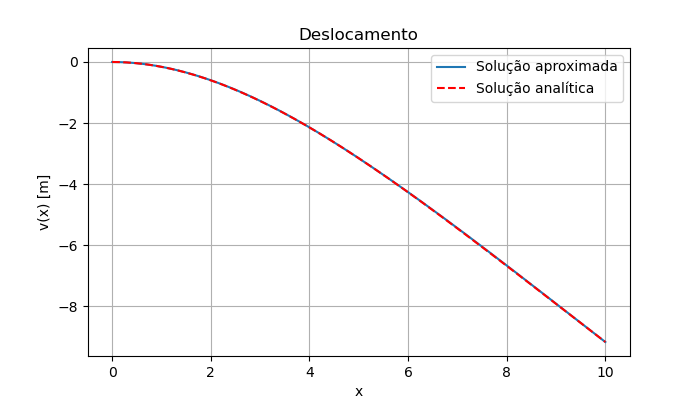
\includegraphics[scale=0.5]{Figures/6-Elemento_viga/deslocamento.png}
                \caption{}
            \end{subfigure}
            ~
            \begin{subfigure}{0.46\textwidth}
                \centering
                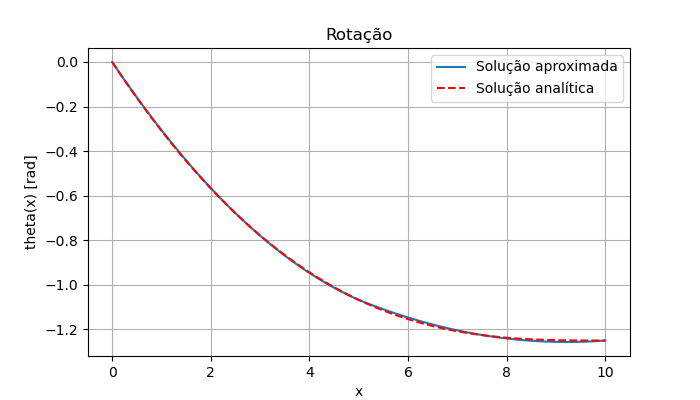
\includegraphics[scale=0.5]{Figures/6-Elemento_viga/rotacao.png}
                \caption{}
            \end{subfigure}\\
            \begin{subfigure}{0.46\textwidth}
                \centering
                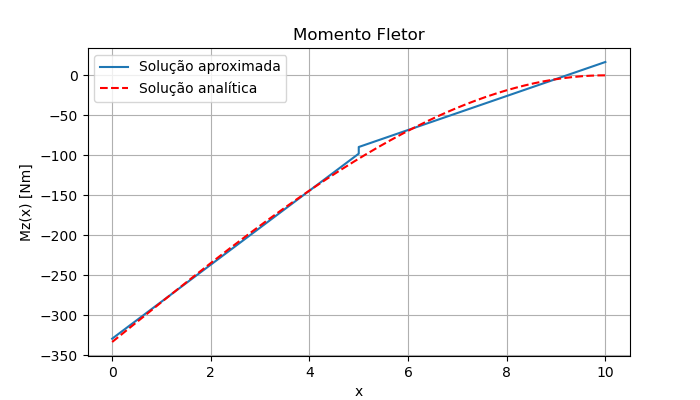
\includegraphics[scale=0.5]{Figures/6-Elemento_viga/fletor.png}
                \caption{}
            \end{subfigure}
            ~
            \begin{subfigure}{0.46\textwidth}
                \centering
                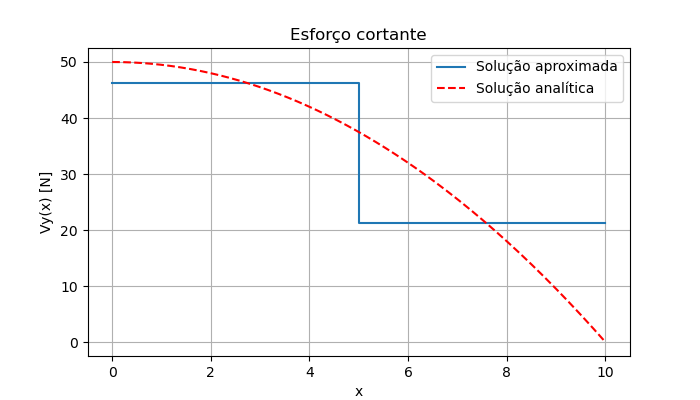
\includegraphics[scale=0.5]{Figures/6-Elemento_viga/cortante.png}
                \caption{}
            \end{subfigure}\\
            \caption{Solução por elementos finitos e analítica do problema de barra. (a) deslocamento, (b) rotação, (c) momento fletor, (d) esforço cortante.}
            \label{fig:exemplo_viga_mef}
        \end{figure}

    \subsection{Elemento de pórtico}

        O elemento de viga e o elemento de barra descrevem o comportamento de um elemento em duas direções diferentes. A barra descreve a tração e a compressão do elemento, e a viga descreve sua flexão. Como ambos os modelos são lineares, podemos considerar um elemento que combine os dois comportamentos pelo princípio da superposição.

        Um elemento de barra possui apenas um grau de liberdade em cada nó (deslocamento $x$), enquanto que o de viga tem dois graus de liberdade (deslocamento $y$ e rotação $\theta_z$). Podemos definir um elemento de pórtico com três graus de liberdade por nó (Figura \ref{fig:portico}).

        \begin{figure}[h!]
            \centering
            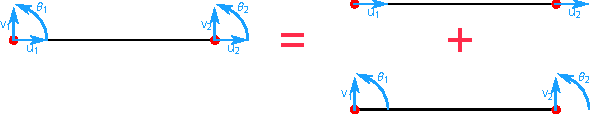
\includegraphics[scale=1.4]{Figures/6-Elemento_viga/Portico.pdf}
            \caption{Elemento de pórtico pela superposição de barra e viga}
            \label{fig:portico}
        \end{figure}

        Por ser um elemento que combina o comportamento dos outros dois, de forma desacoplada, isto é, a barra não modifica o comportamento da viga e vice-versa, podemos apenas concatenar as matrizes de rigidez e os vetores de força:

        \begin{equation}
            \mathbf{K_e}=
            \frac{EA}{h_e}
            \begin{bmatrix}
                1 & 0 & 0 & -1 & 0 & 0\\
                0 & 0 & 0 & 0 & 0 & 0\\
                0 & 0 & 0 & 0 & 0 & 0\\
                -1 & 0 & 0 & 1 & 0 & 0\\
                0 & 0 & 0 & 0 & 0 & 0\\
                0 & 0 & 0 & 0 & 0 & 0\\
            \end{bmatrix}+
            \frac{EI_{zz}}{h_e^3}
            \begin{bmatrix}
                0 & 0 & 0 & 0 & 0 & 0\\
                0 & 12   & 6h_e   & 0 &  -12   & 6h_e   \\
                0 & 6h_e & 4h_e^2 & 0 &  -6h_e & 2h_e^2 \\
                0 & 0 & 0 & 0 & 0 & 0\\
                0 & -12  & -6h_e  & 0 &  12    & -6h_e  \\
                0 & 6h_e & 2h_e^2 & 0 &  -6h_e & 4h_e^2
            \end{bmatrix}
        \end{equation}

        \begin{equation}
            \mathbf{K_e}=
            \begin{bmatrix}
                k_b & 0 & 0 & -k_b & 0 & 0\\
                0 & 12 k_v   & 6h_e k_v   & 0 &  -12k_v   & 6h_e k_v   \\
                0 & 6h_e k_v & 4h_e^2k_v & 0 &  -6h_e k_v & 2h_e^2k_v \\
                -k_b & 0 & 0 & k_b & 0 & 0\\
                0 & -12k_v  & -6h_e k_v  & 0 &  12k_v    & -6h_ek_v \\
                0 & 6h_e k_v & 2h_e^2k_v & 0 &  -6h_e k_v & 4h_e^2k_v 
            \end{bmatrix}
        \end{equation}

        \noindent no qual $k_b = \frac{EA}{h_e}$ e $k_v = \frac{EI_{zz}}{h_e^3}$.

        O sistema, portanto, fica:

        \begin{equation}
            \begin{bmatrix}
                k_b & 0 & 0 & -k_b & 0 & 0\\
                0 & 12 k_v   & 6h_e k_v   & 0 &  -12k_v   & 6h_e k_v   \\
                0 & 6h_e k_v & 4h_e^2k_v & 0 &  -6h_e k_v & 2h_e^2k_v \\
                -k_b & 0 & 0 & k_b & 0 & 0\\
                0 & -12k_v  & -6h_e k_v  & 0 &  12k_v    & -6h_e k_v \\
                0 & 6h_e k_v & 2h_e^2k_v & 0 &  -6h_e k_v & 4h_e^2k_v 
            \end{bmatrix}
            \begin{Bmatrix}
                u_1\\
                v_1\\
                \theta_1\\
                u_2\\
                v_2\\
                \theta_2
            \end{Bmatrix}
            =
            \begin{Bmatrix}
                f_{x_1}\\
                f_{y_1}\\
                m_1\\
                f_{x_2}\\
                f_{y_2}\\
                m_2
            \end{Bmatrix}
        \end{equation}

        O elemento de pórtico, no entanto, nem sempre estará alinhado ao sistema de coordenadas globais. Portanto, considere o elemento da Figura \ref{fig:portico_rotacionado}, que em coordenadas locais está alinhado ao sistema de coordenadas $\bar{x}\bar{y}$. Desejamos obter a matriz de rigidez deste sistema em coordenadas globais $xy$.

        \begin{figure}[h]
            \centering
            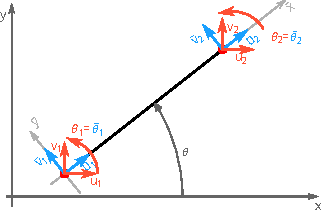
\includegraphics[scale=1.8]{Figures/6-Elemento_viga/Rotacionado.pdf}
            \caption{Elemento de pórtico rotacionado por um ângulo $\theta$}
            \label{fig:portico_rotacionado}
        \end{figure}

        Um vetor no sistema local pode ser transformado ao sistema global multiplicando-o por uma matriz de rotação $\mathbf{R}$:

        \begin{equation}
            \mathbf{\bar{u}} = 
            \begin{Bmatrix}
                \bar{u}\\
                \bar{v}\\
                \bar{\theta}
            \end{Bmatrix}
            =
            \begin{bmatrix}
                \text{cos} \theta & \text{sen} \theta & 0\\
                -\text{sen} \theta & \text{cos} \theta & 0\\
                0 & 0 & 1
            \end{bmatrix}
            \begin{Bmatrix}
                u\\
                v\\
                \theta
            \end{Bmatrix}=
            \mathbf{R} \mathbf{u}
        \end{equation}

        Matrizes de rotação são chamadas \textbf{matrizes ortogonais}. Uma propriedade de matrizes ortogonais é que a sua inversa é igual a sua transposta. O leitor interessado pode verificar essa propriedade na matriz acima ou na matriz de rotação 3D. Portanto, a transformação inversa é dada por:

        \begin{equation}
            \mathbf{u} = \mathbf{R}^T \mathbf{\bar{u}}
        \end{equation}

        Para um dado elemento, podemos escrever a matriz de rotação:

        \begin{equation}
            \mathbf{\bar{u}} = 
            \begin{Bmatrix}
                \bar{u}_1\\
                \bar{v}_1\\
                \bar{\theta}_1\\
                \bar{u}_2\\
                \bar{v}_2\\
                \bar{\theta}_2
            \end{Bmatrix}
            =
            \begin{bmatrix}
                \text{cos} \theta & \text{sen} \theta & 0 & 0 & 0 & 0\\
                -\text{sen} \theta & \text{cos} \theta & 0 & 0 & 0 & 0\\
                0 & 0 & 1 & 0 & 0 & 0\\
                0 & 0 & 0 & \text{cos} \theta & \text{sen} \theta & 0\\
                0 & 0 & 0 & -\text{sen} \theta & \text{cos} \theta & 0\\
                0 & 0 & 0 & 0 & 0 & 1
            \end{bmatrix}
            \begin{Bmatrix}
                u_1\\
                v_1\\
                \theta_1\\
                u_2\\
                v_2\\
                \theta_2\\
            \end{Bmatrix}=
            \mathbf{R}_e \mathbf{u}
        \end{equation}

        O sistema em coordenadas locais pode ser convertido para o sistema em coordenadas globais da seguinte forma:

        \begin{equation*}
            \mathbf{\bar{K}}_e \mathbf{\bar{u}} = \mathbf{\bar{f}}_e
        \end{equation*}

        Pre-multiplicando por $\mathbf{R}^T$ e substituindo a expressão de $mathbf{\bar{u}}$:

        \begin{equation*}
            \mathbf{R}_e^T \mathbf{\bar{K}}_e \mathbf{R}_e \mathbf{u}_e = \mathbf{R}_e^T \mathbf{\bar{f}}_e
        \end{equation*}
        
        \begin{equation*}
            \mathbf{K}_e \mathbf{u}_e = \mathbf{f}_e
        \end{equation*}

        \noindent no qual a matriz então pode ser encontrada como:

        \begin{equation*}
            \mathbf{K}_e = \mathbf{R}_e^T \mathbf{\bar{K}}_e \mathbf{R}_e
        \end{equation*}

        Com relação ao vetor de força, as forças normalmente já são descritas em função do sistema de coordenadas globais, então não é necessária a transformação, neste caso. Entretanto, se a força estiver rotacionada com o elemento, podemos transformá-la de forma similar.

        Finalmente, para o elemento definido pelos pontos $(x_1,y_1)$ e $(x_2,y_2)$, lembre-se que podemos encontrar seu comprimento e ângulo como:

        \begin{equation*}
            h_e = \sqrt{\left(x_2-x_1\right)^2+\left(y_2-y_1\right)^2}
        \end{equation*}

        \begin{equation*}
            \theta_e = \text{tan}^{-1}\left(\frac{y_2-y_1}{x_2-x_1}\right)
        \end{equation*}

        Para o ângulo, devemos nos atentar na programação. Como a função tangente é periódica em $\pi$, usar uma função do tipo \textit{atan()} não é suficiente para obtermos em qual quadrante o ângulo realmente está. Portanto, devemos usar funções do tipo \textit{atan2()}, que também verifica os sinais do denominador e numerador para identificar em qual quadrante o ângulo está.


        Com este elemento de pórtico, podemos resolver sistemas com vários elementos conectados entre si. Por exemplo, se removermos o termo de viga (colocar $k_v=0$ e tirar os graus de liberdade $\theta_z$), podemos montar e resolver um sistema de treliças.

        Portanto, para cada elemento, aplicamos a rotação dele na matriz de rigidez, e montamos no sistema global seguindo o procedimento de montagem mostrado anteriormente.

    \subsection{Exemplo de sistema de pórticos - treliça}

        Considere a treliça da Figura \ref{fig:trelica_ex}. Encontre os deslocamentos dos nós e as tensões em cada barra. Considere que cada barra tem $A = 10^{-5} m$.

        \begin{figure}[h!]
            \centering
            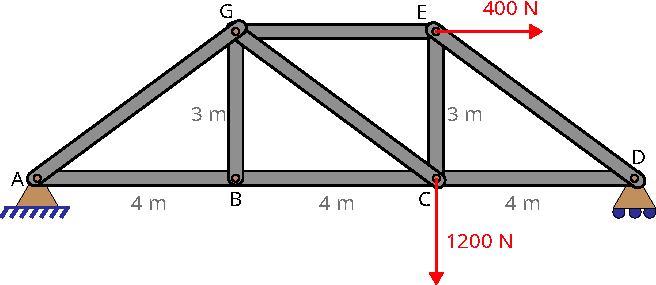
\includegraphics[scale=1]{Figures/6-Elemento_viga/Trelica_exemplo.pdf}
            \caption{Exemplo de problema de treliça}
            \label{fig:trelica_ex}
        \end{figure}

        \subsubsection*{Solução}

        Resolvendo analiticamente, usando equações de equilíbrio da Estática, obtemos as forças de cada barra, e, consequentemente, suas tensões:

        \begin{table}[h!]
            \centering
            \caption{Forças e tensões analíticas do problema de treliça}
            \begin{tabular}{|c|c|c|}
            \hline
            \rowcolor[HTML]{9B9B9B} 
            Barra & Força {[}N{]} & Tensão {[}MPa{]} \\ \hline
            \rowcolor[HTML]{EFEFEF} 
            AB    & 800           & 80               \\ \hline
            \rowcolor[HTML]{FFFFFF} 
            BC    & 800           & 80               \\ \hline
            \rowcolor[HTML]{EFEFEF} 
            CD    & 1200          & 120              \\ \hline
            \rowcolor[HTML]{FFFFFF} 
            DE    & -1500         & -150             \\ \hline
            \rowcolor[HTML]{EFEFEF} 
            EG    & -800          & -80              \\ \hline
            \rowcolor[HTML]{FFFFFF} 
            AG    & -500          & -50              \\ \hline
            \rowcolor[HTML]{EFEFEF} 
            BG    & 0             & 0                \\ \hline
            \rowcolor[HTML]{FFFFFF} 
            CG    & 500           & 50               \\ \hline
            \rowcolor[HTML]{EFEFEF} 
            CE    & 900           & 90               \\ \hline
            \end{tabular}
        \end{table}

        Para resolver por elementos finitos, foi utilizado o programa exemplo\_trelica.py. O deslocamento nodal de cada grau de liberdade, usando a numeração seguindo os nós em ordem alfabética. O mapa de tensões encontrado é mostrado na Figura \ref{fig:ex_trelica_tensao}.

        \begin{figure}[h!]
            \centering
            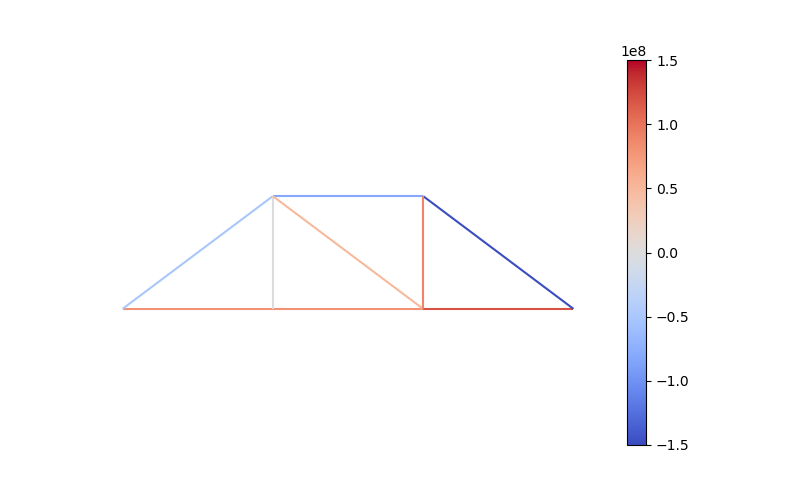
\includegraphics[scale=0.8]{Figures/6-Elemento_viga/tensao_trelica.png}
            \caption{Tensões nas barras. Tensão em Pa.}
            \label{fig:ex_trelica_tensao}
        \end{figure}




    


	%LTeX: language=pt-br
% !TeX root = Apostila_IM381.tex

\cleardoublepage
\section{Problema de condução de calor}
\label{sec:conducao}

    Agora que vimos como o MEF funciona para modelos unidimensionais, vamos passar para o caso bidimensional mais simples: o problema de condução de calor. Os procedimentos usados aqui são os mesmos que para os casos anteriores.

    \subsection{Equação diferencial da condução de calor}

        Considere um domínio $\Omega$ sujeito a uma geração interna de calor $p(x,y)$ (Figura \ref{fig:dominio_calor}). O domínio possui uma condutividade térmica constante de $k$ (se ele for variável, não há alterações significativas na formulação). Em um determinado ponto $\mathbf{x} = \left[x, y\right]^T$ do domínio, o fluxo de calor por área é dada pela lei de Fourier:

        \begin{figure}[h!]
            \centering
            
\includegraphics[scale=1.5]{Figures/7-Calor/Dominio.pdf}
            \caption{Domínio de um problema de condução de calor}
            \label{fig:dominio_calor}
        \end{figure}

        \begin{equation}
            \mathbf{q} = 
            \begin{Bmatrix}
                q_x \\
                q_y \\
            \end{Bmatrix} =
            -k \nabla T = -k 
            \begin{Bmatrix}
                \frac{\partial T}{\partial x} \\
                \frac{\partial T}{\partial y} \\
            \end{Bmatrix}
        \end{equation}

        \noindent no qual o sinal de menos indica que o fluxo de calor segue o sentido de maiores temperaturas para menores.

        Fazendo um balanço de energia em um volume de controle infinitesimal do domínio, considerando temperatura crescente com $x$ e $y$ (Figura \ref{fig:calor_infinitesimal}):

        \begin{figure}[h!]
            \centering
            
\includegraphics[scale=1.4]{Figures/7-Calor/Infinitesimal.pdf}
            \caption{Volume de controle infinitesimal para o balanço de energia do problema de condução}
            \label{fig:calor_infinitesimal}
        \end{figure}

        \begin{equation*}
            q_x dy + q_y dx - q_{x+dx} dy - q_{y+dy} dx + p(x,y) dx dy = 0
        \end{equation*}

        \begin{equation*}
            -k\frac{\partial T}{\partial x} dy 
            -k\frac{\partial T}{\partial y} dx 
            + k\frac{\partial T}{\partial x} dy + \frac{\partial}{\partial x}\left(k\frac{\partial T}{\partial x}\right) dx dy 
            + k\frac{\partial T}{\partial y} dx + \frac{\partial}{\partial y}\left(k\frac{\partial T}{\partial y}\right) dy dx 
            + p(x,y) dx dy = 0
        \end{equation*}

        Portanto, a equação diferencial da condução de calor fica:

        \begin{equation}
            k\frac{\partial^2 T}{\partial x^2}
            +k\frac{\partial^2 T}{\partial y^2}
             = -p(x,y)
        \end{equation}

        Que pode ser escrita com os operadores de divergente ($\nabla \cdot \square$), gradiente ($\nabla \square$) ou o laplaciano, definido como o divergente do gradiente ($\Delta = \nabla \cdot \nabla \square$):

        \begin{equation}
            k \Delta T = k \nabla \cdot \left(\nabla T\right)
             = -p(x,y)
        \end{equation}

        Esta equação também requer condições de contorno ao longo de sua volta completa. Elas podem ser também condições de contorno de Dirichlet, com temperatura imposta em alguma parte de sua superfície:

        \begin{equation}
            T(\mathbf{x}) = T_0 \quad, x \in \Gamma_1 \subset \partial \Omega
        \end{equation}

        \noindent no qual $\Gamma_1$ é alguma superfície no entorno do domínio. O símbolo $\partial \Omega$ representa o fecho (as bordas) do domínio $\Omega$.

        Também pode haver condições de Neumann, representando fluxos de calor impostos na superfície. No caso de condições de contorno, o que importa é o fluxo normal ao fecho do domínio, visto que a tangente é regida pela equação diferencial:

        \begin{equation}
            k\frac{\partial T}{\partial \mathbf{n}} = q_0 \quad, x \in \Gamma_2 \subset \partial \Omega
        \end{equation}

        \noindent no qual $\Gamma_2$ representa uma outra superfície do domínio. O vetor $\mathbf{n}$ é o vetor normal à superfície.

        A condição de contorno mais comum é a de \textbf{superfície adiabática}, ou seja, na qual não há perda de calor para o ambiente. Neste caso, na condição de contorno de Neumann apresentada acima temos $q_0 = 0$.

    \subsection{Forma fraca e aproximação da solução}

        A equação diferencial da forma que obtivemos está na forma forte. Para passarmos para a forma fraca, realizamos o mesmo procedimento que fizemos anteriormente. Inserindo uma função peso $w(x,y)$ no sistema:

        \begin{equation}
            \int_\Omega w(x,y) k \nabla \cdot \left(\nabla T(x,y)\right) dA + \int_\Omega w(x,y) p(x,y) dA = 0 \quad, \forall w(x,y) \in W
            \label{eq:calor_fraca_part1}
        \end{equation}

        Para simplificar as notações, vamos suprimir as dependências por $x$ e $y$. Considere a integral abaixo, podemos utilizar a regra do produto no divergente:

        \begin{equation}
            \int_\Omega \nabla \cdot \left( w\nabla T \right) dA  = 
            \int_\Omega w \nabla \cdot \left(\nabla T\right) dA + 
            \int_\Omega \nabla w^T \nabla T  dA
        \end{equation}

        O primeiro termo pode ser substituído usando o teorema do divergente:

        \begin{equation}
            \int_\Omega \nabla \cdot \left( w\nabla T \right) dA  = 
            \int_{\partial \Omega} w\nabla T \cdot \mathbf{n} d\Gamma
        \end{equation}

        Portanto, temos a seguinte relação ao juntarmos as duas equações:

        \begin{equation}
            \int_\Omega w \nabla \cdot \left(\nabla T\right) dA = 
            \int_{\partial \Omega} w\nabla T \cdot \mathbf{n} d\Gamma -
            \int_\Omega \nabla w \nabla T  dA
        \end{equation}

        Podemos voltar, portanto, para a Eq. \eqref{eq:calor_fraca_part1}:

        \begin{equation*}
            \int_\Omega w k \nabla \cdot \left(\nabla T\right) dA + \int_\Omega w p dA = 0
        \end{equation*}

        \begin{equation*}
            \int_{\partial \Omega} k w\nabla T \cdot \mathbf{n} d\Gamma -
            \int_\Omega k \nabla w^T \nabla T  dA + \int_\Omega w p dA = 0
        \end{equation*}

        \begin{equation}
            \int_\Omega k \nabla w^T \nabla T  dA = 
            \int_{\partial \Omega} k w\nabla T \cdot \mathbf{n} d\Gamma
             + \int_\Omega w p dA \quad ,\forall w \in W
        \end{equation}

        Esta equação representa a forma fraca do problema de condução de calor. Note as similaridades, embora de forma mais complexa, com as equações anteriores. O termo à esquerda da igualdade tem um operador bidirecional entre a função peso e a função incógnita. À direita da igualdade, temos um termo representando as condições de contorno nas interfaces do domínio, e um termo de geração interna, similar ao das forças de campo dos problemas de barra e de viga.

        O próximo passo para a solução é definir um espaço de funções candidatas $T^h(x,y) \in V^h \subset V$ e de funções ponderadoras $w^h(x,y) \in W^h \subset W$. Com o método dos resíduos ponderados, chegamos a uma forma fraca aproximada similar:

        \begin{equation}
            \int_\Omega k \nabla {w^h}^T \nabla T^h  dA = 
            \int_{\partial \Omega} k w^h\nabla T^h \cdot \mathbf{n} d\Gamma
             + \int_\Omega w^h p dA \quad ,\forall w \in W^h
             \label{eq:calor_fraca_aprox}
        \end{equation}


    \subsection{Método de Galerkin}

        Com o método de Galekin, usamos $W^h = V^h$. Portanto, o que nos falta agora é definir quem serão as funções de forma usadas aqui. Já será usada a construção teórica de subdividir o domínio em elementos, estes definidos por funções de forma em suas próprias coordenadas locais. Quais são exatamente essas funções e os domínios, veremos em seguida.

        Considere um elemento cujas coordenadas locais são dadas por $\bar{x}$ e $\bar{y}$. A temperatura e a função teste aproximada no interior desse elemento são interpoladas pelas funções de forma:

        \begin{equation}
            T^h(\bar{x},\bar{y}) = \sum_i N(\bar{x},\bar{y}) a_i = \mathbf{N} \mathbf{a}_e
        \end{equation}

        \begin{equation}
            w^h(\bar{x},\bar{y}) = \sum_i N(\bar{x},\bar{y}) b_i = \mathbf{N} \mathbf{b}_e
        \end{equation}

        No elemento, com um domínio $\Omega_e \subset \Omega$, com uma parte da interface $\Gamma_e \subset \partial \Omega_e$:

        \begin{equation}
            \int_{\Omega_e} k \nabla {w^h}^T \nabla T^h  dA = 
            \int_{\Gamma_e} k w^h\nabla T^h \cdot \mathbf{n} d\Gamma
             + \int_{\Omega_e} w^h p dA \quad ,\forall w \in W^h
             \label{eq:calor_fraca_elemento}
        \end{equation}

        O termo de derivada na primeira integral é o seguinte:

        \begin{equation*}
            \nabla T^h =  
            \begin{Bmatrix}
                \frac{\partial T^h}{\partial x}\\
                \frac{\partial T^h}{\partial y}
            \end{Bmatrix} =
            \begin{Bmatrix}
                \frac{\partial \mathbf{N} \mathbf{a}_e}{\partial x}\\
                \frac{\partial \mathbf{N} \mathbf{a}_e}{\partial y}
            \end{Bmatrix}
        \end{equation*}

        Para transformar este último termo em algo do tipo $\mathbf{B} \mathbf{a}_e$:

        \begin{equation}
            \nabla T^h =  
            \begin{Bmatrix}
                \frac{\partial \mathbf{N} \mathbf{a}}{\partial x}\\
                \frac{\partial \mathbf{N} \mathbf{a}}{\partial y}
            \end{Bmatrix} =
            \begin{bmatrix}
                \frac{\partial \mathbf{N}_1}{\partial x} & \frac{\partial \mathbf{N}_2}{\partial x} & \cdots & \frac{\partial \mathbf{N}_n}{\partial x}\\
                \frac{\partial \mathbf{N}_1}{\partial y} & \frac{\partial \mathbf{N}_2}{\partial y} & \cdots & \frac{\partial \mathbf{N}_n}{\partial y}\\
            \end{bmatrix}
            \begin{Bmatrix}
                a_1\\
                a_2\\
                \vdots\\
                a_n
            \end{Bmatrix}
            = 
            \mathbf{B}
            \mathbf{a}_e
            \label{eq:calor_B}
        \end{equation}


        Analogamente:

        \begin{equation*}
            \nabla w^h =  
            \begin{bmatrix}
                \frac{\partial \mathbf{N}_1}{\partial x} & \frac{\partial \mathbf{N}_2}{\partial x} & \cdots & \frac{\partial \mathbf{N}_n}{\partial x}\\
                \frac{\partial \mathbf{N}_1}{\partial y} & \frac{\partial \mathbf{N}_2}{\partial y} & \cdots & \frac{\partial \mathbf{N}_n}{\partial y}\\
            \end{bmatrix}
            \begin{Bmatrix}
                b_1\\
                b_2\\
                \vdots\\
                b_n
            \end{Bmatrix}
            = 
            \mathbf{B}
            \mathbf{b}_e
        \end{equation*}
        
        Finalmente, voltando à primeira integral da Eq. \eqref{eq:calor_fraca_elemento}:

        \begin{equation*}
            \int_{\Omega_e} k \nabla {w^h}^T \nabla T^h  dA = \mathbf{b}_e^T  k\int_{\Omega_e} \mathbf{B}^T \mathbf{B} dA \;\mathbf{a}_e
        \end{equation*}

        No caso de condução de calor, podemos considerar que:

        \begin{equation}
            \mathbf{D} = 
            \begin{bmatrix}
                k & 0\\
                0 & k
            \end{bmatrix}
        \end{equation}

        Para chegarmos à forma geral:

        \begin{equation*}
            \mathbf{b}_e^T  \int_{\Omega_e} \mathbf{B}^T \mathbf{D} \mathbf{B} dA \; \mathbf{a}_e
        \end{equation*}

        Similarmente para os termos de força:

        \begin{equation}
            \int_{\Gamma_e} k w^h\nabla T^h \cdot \mathbf{n} d\Gamma = -
            \mathbf{b}_e^T  \int_{\Gamma_e} \mathbf{N}^T \left(\mathbf{q} \cdot \mathbf{n}\right) d\Gamma
        \end{equation}

        \begin{equation}
            \int_{\Omega_e} w^h p dA =
            \mathbf{b}_e^T  \int_{\Omega_e} \mathbf{N}^T p(x,y) dA
        \end{equation}

        Portanto, substituindo estes na Eq. \eqref{eq:calor_fraca_elemento}, e sabendo que esta equação deve ser válida para qualquer $\mathbf{b}$, chegamos ao sistema:


        \begin{equation}
            \int_{\Omega_e} \mathbf{B}^T \mathbf{D} \mathbf{B} dA \; \mathbf{a}_e = 
            \int_{\Gamma_e} \mathbf{N}^T \left(\mathbf{q} \cdot \mathbf{n}\right) d\Gamma +
            \int_{\Omega_e} \mathbf{N}^T p(x,y) dA
            \label{eq:calor_eq_elemento}
        \end{equation}


        \begin{equation}
            \mathbf{K}_e \mathbf{a}_e = \mathbf{f}_e
        \end{equation}

        Da mesma forma como anteriormente, realizamos a montagem do sistema global a partir das matrizes elementares. Resolvemos o sistema global:

        \begin{equation}
            \mathbf{K} \mathbf{a} = \mathbf{f},
        \end{equation}

        \noindent que nos retorna os coeficientes que usamos para reconstruir o campo de temperatura do domínio, interpolando em cada elemento.

        Com os coeficientes, podemos calcular também os fluxos de calor por unidade de área:

        \begin{equation}
            \mathbf{q}(\bar{x},\bar{y}) = - k \nabla T^h = - \mathbf{D} \mathbf{B} \mathbf{a}_e
            \label{eq:fluxo_reconstruido}
        \end{equation}


    \subsection{Elemento triangular regular}
    \label{sec:elemento_triangular}

        O elemento com a formulação mais simples, embora em alguns aspectos seja relativamente complexo, é o triângulo. Considere o elemento triangular da Figura \ref{fig:element_triangulo}, as coordenadas locais em elementos deste tipo são normalmente definidas pelas três áreas ($A_1$, $A_2$ e $A_3$) definidas pelos três vértices e o ponto interno.

        \begin{figure}[h!]
            \centering
            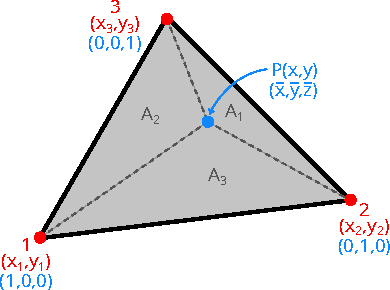
\includegraphics[scale=1.4]{Figures/7-Calor/Triangulo.pdf}
            \caption{Elemento triangular definido pelas coordenadas locais}
            \label{fig:element_triangulo}
        \end{figure}

        As coordenadas locais $\bar{x}$, $\bar{y}$ e $\bar{z}$ (não confunda a nomenclatura aqui como um sistema em três dimensões) podem ser definidas como:

        \begin{equation}
            \bar{x} = \frac{A_1}{A} \quad \bar{y} = \frac{A_2}{A} \quad \bar{z} = \frac{A_3}{A}
        \end{equation}

        \noindent no qual $A = A_1 + A_2 + A_3$. Portanto, $\bar{x} + \bar{y} + \bar{z} = 1$ e, consequentemente:

        \begin{equation}
            \bar{z} = 1 - \bar{x} - \bar{y}
        \end{equation}

        As coordenadas globais em um ponto qualquer é dado por:

        \begin{equation}
            x = \bar{x} x_1 + \bar{y} x_2 + \bar{z} x_3 = \sum_i N_i x_i
        \end{equation}

        \begin{equation}
            y = \bar{x} y_1 + \bar{y} y_2 + \bar{z} y_3 = \sum_i N_i y_i
        \end{equation}

        \begin{equation}
            \mathbf{x} = 
            \begin{Bmatrix}
                x\\
                y
            \end{Bmatrix} = 
            \mathbf{N} \mathbf{x_n}
        \end{equation}

        \noindent no qual $\mathbf{x_n}^T = 
        \begin{bmatrix}
                x_1 &
                y_1 &
                x_2 &
                y_2 &
                x_3 &
                y_3 &
            \end{bmatrix}$ e $ 
            \mathbf{N} = 
            \begin{bmatrix}
                \bar{x} &
                \bar{x} &
                \bar{y} &
                \bar{y} &
                1 - \bar{x} - \bar{y} &
                1 - \bar{x} - \bar{y}
            \end{bmatrix}$. Isto é, $N_1(\bar{x},\bar{y}) = \bar{x}$, $N_2(\bar{x},\bar{y}) = \bar{y}$ e $N_3(\bar{x},\bar{y}) = 1 - \bar{x} - \bar{y}$. Essas funções de forma têm a mesma propriedade dos polinômios de Lagrange, isto é, quando usadas para interpolar as temperaturas, os coeficientes do sistema representam as temperaturas nos nós correspondentes a cada uma dessas funções de forma. Note que neste caso, no entanto, não há a propriedade de superconvergência, então as temperaturas nodais não serão exatas.

        As derivadas das coordenadas globais em relação a cada coordenada local é dada por:

        \begin{equation*}
            \frac{\partial x}{\partial \bar{x}} = x_1 - x_3 \quad \frac{\partial x}{\partial \bar{y}} = x_2 - x_3
            \quad \frac{\partial y}{\partial \bar{x}} = y_1 - y_3 \quad \frac{\partial y}{\partial \bar{y}} = y_2 - y_3
        \end{equation*}

        Podemos definir uma matriz chamada \textbf{Jacobiano}:

        \begin{equation}
            \mathbf{J} = 
            \begin{bmatrix}
                 \frac{\partial x}{\partial \bar{x}} &  \frac{\partial y}{\partial \bar{x}}\\
                 \frac{\partial x}{\partial \bar{y}} &  \frac{\partial y}{\partial \bar{y}}
            \end{bmatrix}
        \end{equation}

        \noindent cujo determinante aqui é dado por:

        \begin{equation}
            \det \mathbf{J} = \left(x_1 - x_3\right)\left(y_2 - y_3\right) - \left(x_2 - x_3\right)\left(y_1 - y_3\right) = 2A
        \end{equation}

        A derivada de uma função qualquer $f(x,y)$ em relação às coordenadas locais e às globais podem ser relacionadas pela regra da cadeia:

        \begin{equation*}
            \frac{\partial f}{\partial \bar{x}} = 
            \frac{\partial f}{\partial x} \frac{\partial x}{\partial \bar{x}} + 
            \frac{\partial f}{\partial y} \frac{\partial y}{\partial \bar{x}} =
            \begin{bmatrix}
                \frac{\partial x}{\partial \bar{x}} &
                \frac{\partial y}{\partial \bar{x}}
            \end{bmatrix}
            \begin{Bmatrix}
                \frac{\partial f}{\partial x} \\
                \frac{\partial f}{\partial y}
            \end{Bmatrix}
        \end{equation*}

        \begin{equation*}
            \frac{\partial f}{\partial \bar{y}} = 
            \frac{\partial f}{\partial x} \frac{\partial x}{\partial \bar{y}} + 
            \frac{\partial f}{\partial y} \frac{\partial y}{\partial \bar{y}} =
            \begin{bmatrix}
                \frac{\partial x}{\partial \bar{y}} &
                \frac{\partial y}{\partial \bar{y}}
            \end{bmatrix}
            \begin{Bmatrix}
                \frac{\partial f}{\partial x} \\
                \frac{\partial f}{\partial y}
            \end{Bmatrix}
        \end{equation*}

        \begin{equation}
            \begin{Bmatrix}
                \frac{\partial f}{\partial \bar{x}} \\
                \frac{\partial f}{\partial \bar{y}}
            \end{Bmatrix} =
            \begin{bmatrix}
                \frac{\partial x}{\partial \bar{x}} & \frac{\partial y}{\partial \bar{x}}\\
                \frac{\partial x}{\partial \bar{y}} & \frac{\partial y}{\partial \bar{y}}
            \end{bmatrix}
            \begin{Bmatrix}
                \frac{\partial f}{\partial x} \\
                \frac{\partial f}{\partial y}
            \end{Bmatrix}
            = \mathbf{J}
            \begin{Bmatrix}
                \frac{\partial f}{\partial x} \\
                \frac{\partial f}{\partial y}
            \end{Bmatrix}
        \end{equation}
        

        \begin{equation}
            \begin{Bmatrix}
                \frac{\partial f}{\partial x} \\
                \frac{\partial f}{\partial y}
            \end{Bmatrix} = 
            \mathbf{J}^{-1}
            \begin{Bmatrix}
                \frac{\partial f}{\partial \bar{x}} \\
                \frac{\partial f}{\partial \bar{y}}
            \end{Bmatrix}
        \end{equation}

        No problema térmico, como verificamos anteriormente, precisamos das derivadas das funções de forma em relação às coordenadas globais. Elas podem ser obtidas desta forma:

        \begin{equation}
            \begin{Bmatrix}
                \frac{\partial N_1}{\partial x} \\
                \frac{\partial N_1}{\partial y}
            \end{Bmatrix} = 
            \mathbf{J}^{-1}
            \begin{Bmatrix}
                \frac{\partial N_1}{\partial \bar{x}} \\
                \frac{\partial N_1}{\partial \bar{y}}
            \end{Bmatrix} = 
            \mathbf{J}^{-1}
            \begin{Bmatrix}
                1 \\
                0
            \end{Bmatrix}
            \quad 
            \begin{Bmatrix}
                \frac{\partial N_2}{\partial x} \\
                \frac{\partial N_2}{\partial y}
            \end{Bmatrix} = 
            \mathbf{J}^{-1}
            \begin{Bmatrix}
                0 \\
                1
            \end{Bmatrix}
            \quad
            \begin{Bmatrix}
                \frac{\partial N_3}{\partial x} \\
                \frac{\partial N_3}{\partial y}
            \end{Bmatrix} = 
            \mathbf{J}^{-1}
            \begin{Bmatrix}
                -1 \\
                -1
            \end{Bmatrix}
        \end{equation}

        Resolvendo estes sistemas, obtemos as seguintes derivadas:

        \begin{equation*}
            \frac{\partial N_1}{\partial x} = \frac{y_2-y_3}{2A} \quad,
            \frac{\partial N_2}{\partial x} = \frac{y_3-y_1}{2A} \quad,
            \frac{\partial N_3}{\partial x} = \frac{y_1-y_2}{2A}
        \end{equation*}

        \begin{equation}
            \frac{\partial N_1}{\partial y} = \frac{x_3-x_2}{2A} \quad,
            \frac{\partial N_2}{\partial y} = \frac{x_1-x_3}{2A} \quad,
            \frac{\partial N_3}{\partial y} = \frac{x_2-x_1}{2A}
        \end{equation}

        Note que todos esses valores são \textbf{constantes}. Portanto, com eles, podemos montar a matriz $\mathbf{B}$ do problema de condução de calor, conforme a Eq. \eqref{eq:calor_B}.

        Finalmente, retornamos à integral da matriz de rigidez:

        \begin{equation*}
            \mathbf{K}_e = \int_{\Omega_e} \mathbf{B}^T \mathbf{D} \mathbf{B} dA
        \end{equation*}

        Em um domínio de ordem superior, a transformação de coordenadas é dada a partir da transformação dos dois integrandos ($dx$ e $dy$), nos integrandos ($d\bar{x}$ e $d\bar{y}$). O termo de derivada de um em relação ao outro é dado pelo \textbf{determinante do Jacobiano}. Finalmente, lembre-se que $\bar{x} + \bar{y} + \bar{z} = 1$. Portanto, o limite superior de integração para $\bar{y}$ deve ser $1-\bar{x}$, para não ultrapassar o limite.

        \begin{equation*}
            \int_{\Omega_e} \mathbf{B}^T \mathbf{D} \mathbf{B} dA = \int_{0}^{1} \int_{0}^{1-\bar{x}} \mathbf{B}^T \mathbf{D} \mathbf{B} \det \mathbf{J} d\bar{y} d\bar{x}
        \end{equation*}

        Todos os termos na integral são constantes, tanto em relação a $\bar{x}$ quanto a $\bar{y}$, portanto:


        \begin{equation}
            \mathbf{K}_e = \mathbf{B}^T \mathbf{D} \mathbf{B} \det \mathbf{J} \int_{0}^{1} \int_{0}^{1-\bar{x}}  d\bar{y} d\bar{x} = \frac{1}{2} \mathbf{B}^T \mathbf{D} \mathbf{B} \det \mathbf{J}
        \end{equation}


        O fluxo de calor dentro do elemento é dado pela Eq. \eqref{eq:fluxo_reconstruido}:

        \begin{equation*}
            \mathbf{q} = - k \nabla T^h = - \mathbf{D} \mathbf{B} \mathbf{a}_e
        \end{equation*}

        O fluxo de calor dentro de um elemento triangular será constante. Uma consequência é que na interface entre dois elementos, haverá uma descontinuidade no fluxo também.

        Sobre os termos de força, podemos integrá-los também. O termo da interface pode ser integrado como se fossem elementos unidimensionais, com sua variável sendo a parametrização desta superfície. O termo de geração de carga também pode ser integrada. Considere um caso com geração uniforme $p(x,y) = Q$:


        \begin{equation*}
            \int_{\Omega_e} \mathbf{N}^T Q dA = 
            Q \int_{0}^{1} \int_{0}^{1-\bar{x}} 
            \begin{Bmatrix}
                \bar{x}\\
                \bar{y}\\
                1-\bar{x}-\bar{y}
            \end{Bmatrix} \det \mathbf{J} d\bar{y} d\bar{x} = 
            Q \det \mathbf{J} \int_{0}^{1} \left.
            \begin{Bmatrix}
                \bar{x}\bar{y}\\
                \bar{y}^2/2\\
                \bar{y}-\bar{x}\bar{y}-\bar{y}^2/2
            \end{Bmatrix} \right|_{0}^{1-\bar{x}}  d\bar{x}
        \end{equation*}

        \begin{equation*}
             \int_{\Omega_e} \mathbf{N}^T Q dA = 2QA\int_{0}^{1} 
            \begin{Bmatrix}
                \bar{x}-\bar{x}^2\\
                1/2 - \bar{x} + \bar{x}^2/2\\
                1/2 - \bar{x} + \bar{x}^2/2
            \end{Bmatrix}  d\bar{x} = 
             2QA \left.
            \begin{Bmatrix}
                \bar{x}^2/2-\bar{x}^3/3\\
                \bar{x}/2 - \bar{x}^2/2 + \bar{x}^3/6\\
                \bar{x}/2 - \bar{x}^2/2 + \bar{x}^3/6
            \end{Bmatrix}  \right|_{0}^{1} 
        \end{equation*}

        \begin{equation*}
             \int_{\Omega_e} \mathbf{N}^T Q dA =
             \frac{QA}{3}
            \begin{Bmatrix}
                1\\
                1\\
                1
            \end{Bmatrix}
        \end{equation*}



	%LTeX: language=pt-br
% !TeX root = Apostila_IM381.tex

\cleardoublepage
\section{Estado plano}
\label{sec:estado_plano}

    \subsection{Equilíbrio 2D}

        Considere o domínio da Figura \ref{fig:dominio_elastico}, sujeito a forças externas aplicadas, forças de campo $\mathbf{b}(x,y)$ e a condições de contorno. Considerando um elemento infinitesimal (Figura \ref{fig:equilíbrio}), aparecem os termos de tensão, que descrevem o equilíbrio:

        \begin{figure}[h!]
            \centering
            
\includegraphics[scale=1.4]{Figures/8-Plano/Dominio.pdf}
            \caption{Domínio de uma estrutura linear elástica sujeita a forças externas}
            \label{fig:dominio_elastico}
        \end{figure}

        \begin{figure}[h!]
            \centering
            
\includegraphics[scale=1.4]{Figures/8-Plano/Infinitesimal.pdf}
            \caption{Equilíbrio de um elemento infinitesimal na estrutura}
            \label{fig:equilíbrio}
        \end{figure}

        \begin{equation*}
            \sum F_x = 0 
        \end{equation*}

        \begin{equation*}
            -\sigma_{xx}dy - \tau_{xy}dx + 
            \left(\sigma_{xx} + \frac{\partial \sigma_{xx}}{\partial x} dx\right) dy +
            \left(\tau_{xy} + \frac{\partial \tau_{xy}}{\partial y} dy\right) dx +
            b_x(x,y) dx dy = 0
        \end{equation*}

        \begin{equation*}
            \frac{\partial \sigma_{xx}}{\partial x} +
            \frac{\partial \tau_{xy}}{\partial y} +
            b_x(x,y) = 0
        \end{equation*}


        \begin{equation*}
            \sum F_y = 0
        \end{equation*}

        \begin{equation*}
            -\sigma_{yy}dx - \tau_{xy}dy + 
            \left(\sigma_{yy} + \frac{\partial \sigma_{yy}}{\partial y} dy\right) dx +
            \left(\tau_{xy} + \frac{\partial \tau_{xy}}{\partial x} dx\right) dy +
            b_y(x,y) dx dy = 0
        \end{equation*}

        \begin{equation*}
            \frac{\partial \tau_{xy}}{\partial x} +
            \frac{\partial \sigma_{yy}}{\partial y} +
            b_y(x,y) = 0
        \end{equation*}

        Portanto, temos o sistema:

        \begin{equation}
            \left\{
            \begin{array}{l}
                 \frac{\partial \sigma_{xx}}{\partial x} + \frac{\partial \tau_{xy}}{\partial y} + b_x(x,y) = 0\\
                 \frac{\partial \tau_{xy}}{\partial x} + \frac{\partial \sigma_{yy}}{\partial y} + b_y(x,y) = 0
            \end{array}
            \right.
            \label{eq:equilibrio2D}
        \end{equation}

        No caso geral 3D, teríamos a seguinte equação:

        \begin{equation}
            \left\{
            \begin{array}{l}
                 \frac{\partial \sigma_{xx}}{\partial x} + \frac{\partial \tau_{xy}}{\partial y} + \frac{\partial \tau_{xz}}{\partial z} + b_x(x,y,z) = 0\\
                 \frac{\partial \tau_{xy}}{\partial x} + \frac{\partial \sigma_{yy}}{\partial y} + \frac{\partial \tau_{yz}}{\partial z} + b_y(x,y,z) = 0\\
                 \frac{\partial \tau_{xz}}{\partial x} + \frac{\partial \tau_{yz}}{\partial y} + \frac{\partial \sigma_{zz}}{\partial z} + b_z(x,y,z) = 0
            \end{array}
            \right.
        \end{equation}

        Podemos escrever em uma única equação como:

        \begin{equation}
            \nabla \cdot \mathbf{T} + \mathbf{b} = \mathbf{0}
            \label{eq:equilibrio}
        \end{equation}

        \noindent no qual $\mathbf{T}$ é o tensor de tensão de Cauchy:

        \begin{equation*}
            \mathbf{T} = 
            \begin{bmatrix}
                \sigma_{xx} & \tau_{xy}   & \tau_{xz}\\
                \tau_{xy}   & \sigma_{yy} & \tau_{yz}\\
                \tau_{xz}   & \tau_{yz}   & \sigma_{zz}
            \end{bmatrix}
        \end{equation*}

    \subsection{Modelos constitutivos}

        Outra notação para as tensões e deformações é a chamada notação de Voigt, no qual as componentes de tensão e deformação são escritas como um vetor, em vez de um tensor.

        À relação entre tensão e deformação, dá-se o nome de equação constitutiva. Estudaremos aqui dois modelos, ambos usados para simular o comportamento de estruturas de forma 2D. Os modelos apresentados aqui são o estado plano de tensão e o estado plano de deformação. Ambos os modelos são caracterizados por materiais lineares elásticos e isotrópicos, sujeitos a pequenas deformações e deslocamentos.

        O estado plano de tensão é usado para modelar corpos finos, nos quais podemos adotar a hipótese que quaisquer tensões na direção fina (eixo $z$) serão muito menores que as tensões nas outras direções. A relação entre as tensões e deformações no plano $xy$ é:

        \begin{equation}
            \begin{Bmatrix}
                \sigma_{xx}\\
                \sigma_{yy}\\
                \tau_{xy}\\
            \end{Bmatrix}
            =
            \frac{E}{1-\nu^2}
            \begin{bmatrix}
                1 & \nu & 0\\
                \nu & 1 & 0\\
                0 & 0 & \frac{1-\nu}{2}
            \end{bmatrix}
            \begin{Bmatrix}
                \varepsilon_{xx}\\
                \varepsilon_{yy}\\
                \gamma_{xy}\\
            \end{Bmatrix}
        \end{equation}

        \begin{equation}
            \bm{\sigma} =
            \mathbf{D}
            \bm{\varepsilon}
        \end{equation}


        \noindent no qual $E$ é o módulo de Young e $\nu$ é o coeficiente de Poisson do material.

        O estado plano de deformação é usado para modelar corpos espessos, como pontes e barragens, nos quais podemos adotar a hipótese que quaisquer deformações na direção espessa (eixo $z$) serão muito menores que as deformações nas outras direções. A relação entre as tensões e deformações no plano $xy$ é:

        \begin{equation*}
            \begin{Bmatrix}
                \sigma_{xx}\\
                \sigma_{yy}\\
                \tau_{xy}\\
            \end{Bmatrix}
            =
            \frac{E}{\left(1+\nu\right)\left(1-2\nu\right)}
            \begin{bmatrix}
                1-\nu & \nu & 0\\
                \nu & 1-\nu & 0\\
                0 & 0 & \frac{1-2\nu}{2}
            \end{bmatrix}
            \begin{Bmatrix}
                \varepsilon_{xx}\\
                \varepsilon_{yy}\\
                \gamma_{xy}\\
            \end{Bmatrix}
        \end{equation*}

        \begin{equation}
            \bm{\sigma} =
            \mathbf{D}
            \bm{\varepsilon}
        \end{equation}

    \subsection{Cinemática}

        As deformações, por sua vez, podem ser correlacionadas com os deslocamentos da estrutura. A função incógnita do problema de equilíbrio estático é o campo de deslocamento $\mathbf{u}$ da estrutura, que possui componentes em cada direção, no caso 2D:

        \begin{equation}
            \mathbf{u}(\mathbf{x}) = 
            \begin{Bmatrix}
                u(\mathbf{x})\\
                v(\mathbf{x})
            \end{Bmatrix},
        \end{equation}

        \noindent enquanto que no 3D, aparece um deslocamento $w(\mathbf{x})$ no eixo $z$.

        O tensor de deformação infinitesimal é dado por:
        
        \begin{equation*}
            \mathbf{E} = 
            \begin{bmatrix}
                \varepsilon_{xx} & \varepsilon_{xy} & \varepsilon_{xz}\\
                \varepsilon_{xy} & \varepsilon_{yy} & \varepsilon_{yz}\\
                \varepsilon_{xz} & \varepsilon_{yz} & \varepsilon_{zz}
            \end{bmatrix}
            = \frac{1}{2} \left(\nabla \mathbf{u} + \nabla \mathbf{u}^T\right)=
            \begin{bmatrix}
                \frac{\partial u}{\partial x} & 
                \frac{1}{2} \left( \frac{\partial u}{\partial y} + \frac{\partial v}{\partial x} \right) & 
                \frac{1}{2} \left( \frac{\partial u}{\partial z} + \frac{\partial w}{\partial x} \right)\\
                \frac{1}{2} \left( \frac{\partial u}{\partial y} + \frac{\partial v}{\partial x} \right) & 
                \frac{\partial v}{\partial y} & 
                \frac{1}{2} \left( \frac{\partial v}{\partial z} + \frac{\partial w}{\partial y} \right)\\
                \frac{1}{2} \left( \frac{\partial u}{\partial z} + \frac{\partial w}{\partial x} \right) & 
                \frac{1}{2} \left( \frac{\partial v}{\partial z} + \frac{\partial w}{\partial y} \right) & 
                \frac{\partial w}{\partial z}
            \end{bmatrix}
            \label{eq:deformacao_green}
        \end{equation*}

        Na notação de Voigt, no 2D, sabendo que $\gamma_{xy} = 2\varepsilon_{xy}$, $\gamma_{xz} = 2\varepsilon_{xz}$ e $\gamma_{yz} = 2\varepsilon_{yz}$:

        \begin{equation}
            \begin{Bmatrix}
                \varepsilon_{xx}\\
                \varepsilon_{yy}\\
                \gamma_{xy}\\
            \end{Bmatrix}
            =
            \begin{Bmatrix}
                \frac{\partial u}{\partial x}\\
                \frac{\partial v}{\partial y}\\
                \frac{\partial u}{\partial y} + \frac{\partial v}{\partial x}\\
            \end{Bmatrix}
            =
            \begin{bmatrix}
                \frac{\partial}{\partial x} & 0\\
                0 & \frac{\partial}{\partial y}\\
                \frac{\partial}{\partial y} & \frac{\partial}{\partial x}\\
            \end{bmatrix}
            \begin{Bmatrix}
                u\\
                v\\
            \end{Bmatrix}
            =
            \mathbf{B}_L
            \mathbf{u}
            \label{eq:voigt_deformacao}
        \end{equation}


    \subsection{Forma fraca}

        Voltando à equação de equilíbrio (Eq. \eqref{eq:equilibrio}). As funções candidatas $\mathbf{u}(\mathbf{x})$ se encontram no espaço $V$. Considere agora também uma função peso, que também é uma função vetorial de mesma dimensão, $\mathbf{w}(\mathbf{x})$, no espaço $W$. Desta forma, temos a condição:

        \begin{equation}
            \int_\Omega \mathbf{w} \cdot \left(\nabla \cdot \mathbf{T}\right)dA + \int_\Omega \mathbf{w} \cdot \mathbf{b} = 0
            \label{eq:elastico_fraca_part1}
        \end{equation}

        Vamos utilizar a relação:

        \begin{equation}
            \nabla \cdot \left(\mathbf{w} \cdot \mathbf{T}\right) = \mathbf{w} \cdot \left(\nabla \cdot \mathbf{T}\right) + \nabla\mathbf{w} : \mathbf{T}
        \end{equation}

        \noindent no qual as operações entre vetor e matriz mostradas aqui são as seguintes: o produto escalar  entre um vetor e matriz ($\mathbf{w} \cdot \mathbf{T}$) é definido como um vetor que contém o produto escalar entre o vetor com cada coluna da matriz. O produto dois pontos entre duas matrizes, é o produto escalar entre duas matrizes, a soma do produto termo a termo de cada matriz.

        Como o tensor $\mathbf{T}$ é simétrico, teremos que:

        \begin{equation}
            \nabla \cdot \left(\mathbf{w} \cdot \mathbf{T}\right) = \mathbf{w} \cdot \left(\nabla \cdot \mathbf{T}\right) + \left[\frac{\nabla\mathbf{w} + \nabla\mathbf{w}^T}{2}\right] : \mathbf{T}
        \end{equation}

        Notando a similaridade com a Eq. \eqref{eq:deformacao_green}:

        \begin{equation}
            \nabla \cdot \left(\mathbf{w} \cdot \mathbf{T}\right) = \mathbf{w} \cdot \left(\nabla \cdot \mathbf{T}\right) + \mathbf{E}_w : \mathbf{T}
        \end{equation}


        Integrando essa equação e usando o teorema do divergente:

        \begin{equation*}
            \int_\Omega \nabla \cdot \left(\mathbf{w} \cdot \mathbf{T}\right)dA = 
            \int_\Omega \mathbf{w} \cdot \left(\nabla \cdot \mathbf{T}\right)dA +
            \int_\Omega \mathbf{E}_w : \mathbf{T} \; dA
        \end{equation*}

        \begin{equation*}
            \int_{\partial \Omega} \mathbf{w} \cdot \mathbf{T} \cdot \mathbf{n} \; d\Gamma = 
            \int_\Omega \mathbf{w} \cdot \left(\nabla \cdot \mathbf{T}\right)dA +
            \int_\Omega \mathbf{E}_w : \mathbf{T} \; dA
        \end{equation*}

        \begin{equation*}
            \int_{\partial \Omega} \mathbf{w} \cdot \mathbf{t} \; d\Gamma = 
            \int_\Omega \mathbf{w} \cdot \left(\nabla \cdot \mathbf{T}\right)dA +
            \int_\Omega \mathbf{E}_w : \mathbf{T} \; dA
        \end{equation*}

        \begin{equation}
            \int_\Omega \mathbf{w} \cdot \left(\nabla \cdot \mathbf{T}\right)dA = 
            \int_{\partial \Omega} \mathbf{w} \cdot \mathbf{t} \; d\Gamma -
            \int_\Omega \mathbf{E}_w : \mathbf{T} \; dA
        \end{equation}

        \noindent no qual $\mathbf{t}$ são as forças superficiais que aparecem em uma determinada seção da estrutura, no caso, normal à superfície $d\Gamma$.

        Retornando, então à Eq \eqref{eq:elastico_fraca_part1}:

        \begin{equation}
            \int_\Omega \mathbf{E}_w : \mathbf{T} \; dA = \int_{\partial \Omega} \mathbf{w}^T \mathbf{t} \; d\Gamma + \int_\Omega \mathbf{w}^T \mathbf{b} \; dA
            \label{eq:elastico_fraca_part2}
        \end{equation}

        Podemos reescrever a primeira integral, usando a notação de Voigt, em vez de usar vetores. Usaremos a relação das Eq. \eqref{eq:voigt_deformacao}:

        \begin{equation}
            \int_\Omega \mathbf{E}_w : \mathbf{T} \; dA = \int_\Omega \bm{\varepsilon}_w^T \bm{\sigma} dA =  \int_\Omega \mathbf{w}^T \mathbf{B}_L^T \mathbf{D} \mathbf{B}_L \mathbf{u} dA
        \end{equation}

        Portanto, a forma fraca deste sistema fica:

        \begin{equation}
            \int_\Omega \mathbf{w}^T \mathbf{B}_L^T \mathbf{D} \mathbf{B}_L \mathbf{u} dA = \int_{\partial \Omega} \mathbf{w}^T \mathbf{t} \; d\Gamma + \int_\Omega \mathbf{w}^T \mathbf{b} \; dA \quad, \forall \mathbf{w} \in W
            \label{eq:elastico_fraca}
        \end{equation}

    \subsection{Resíduos ponderados e funções de forma}

        Agora, consideremos uma solução aproximada $\mathbf{u}^h(\mathbf{x}) \in V^h$ e funções peso que pertencem a um espaço $W^h$ gerado pelas mesmas funções (método de Galerkin):

        \begin{equation}
            \int_\Omega {\mathbf{w}^h}^T \mathbf{B}_L^T \mathbf{D} \mathbf{B}_L \mathbf{u}^h dA = \int_{\partial \Omega} {\mathbf{w}^h}^T \mathbf{t} \; d\Gamma + \int_\Omega {\mathbf{w}^h}^T \mathbf{b} \; dA \quad, \forall \mathbf{w}^h \in W^h
        \end{equation}

        A solução é aproximada novamente por funções de forma. Entretanto, neste caso, como o campo de deslocamento é vetorial, cada componente é interpolado:

        \begin{equation}
            u^h(\mathbf{x}) = \sum_i N_i(\mathbf{x}) u_i
        \end{equation}

        \begin{equation}
            v^h(\mathbf{x}) = \sum_i N_i(\mathbf{x}) v_i
        \end{equation}

        \begin{equation}
            \mathbf{u}^h(\mathbf{x}) = 
            \begin{Bmatrix}
                u^h(\mathbf{x})\\
                v^h(\mathbf{x})
            \end{Bmatrix} =
            \begin{bmatrix}
                N_1 & 0 & N_2 & 0 & \cdots & N_n & 0\\
                0 & N_1 & 0 & N_2 & 0 & \cdots & 0 & N_n\\
            \end{bmatrix}
            \begin{Bmatrix}
                u_1\\
                v_1\\
                u_2\\
                v_2\\
                \vdots\\
                u_n\\
                v_n\\
            \end{Bmatrix} =
            \mathbf{N}(\mathbf{x})
            \mathbf{a}
        \end{equation}

        \begin{equation}
            \mathbf{w}^h(\mathbf{x}) = 
            \mathbf{N}(\mathbf{x})
            \mathbf{m}
        \end{equation}

        Com as funções de forma, os termos com $\mathbf{B}_L$ das integrais ficam:

        \begin{equation*}
            \mathbf{B}_L \mathbf{u}^h = 
             \begin{bmatrix}
                \frac{\partial}{\partial x} & 0\\
                0 & \frac{\partial}{\partial y}\\
                \frac{\partial}{\partial y} & \frac{\partial}{\partial x}\\
            \end{bmatrix}
            \begin{bmatrix}
                N_1 & 0 & N_2 & 0 & \cdots & N_n & 0\\
                0 & N_1 & 0 & N_2 & 0 & \cdots & 0 & N_n\\
            \end{bmatrix}
            \begin{Bmatrix}
                u_1\\
                v_1\\
                u_2\\
                v_2\\
                \vdots\\
                u_n\\
                v_n\\
            \end{Bmatrix}
        \end{equation*}

        \begin{equation}
            \mathbf{B}_L \mathbf{u}^h = 
             \begin{bmatrix}
                \frac{\partial N_1}{\partial x} & 0 & \cdots & \frac{\partial N_n}{\partial x} & 0\\
                0 & \frac{\partial N_1}{\partial y} & \cdots & 0 & \frac{\partial N_n}{\partial y}\\
                \frac{\partial N_1}{\partial y} & \frac{\partial N_1}{\partial x} & \cdots & \frac{\partial N_n}{\partial y} & \frac{\partial N_n}{\partial x}\\
            \end{bmatrix}
            \begin{Bmatrix}
                u_1\\
                v_1\\
                u_2\\
                v_2\\
                \vdots\\
                u_n\\
                v_n\\
            \end{Bmatrix}
            =
            \mathbf{B}
            \mathbf{a}
        \end{equation}

        Portanto, a forma fraca aproximada, já substituindo os valores de $\mathbf{B}$, fica:

        \begin{equation}
            \mathbf{m}^T\int_\Omega  \mathbf{B}^T \mathbf{D} \mathbf{B} dA \; \mathbf{a} = \mathbf{b}^T \int_{\partial \Omega} \mathbf{N}^T \mathbf{t} \; d\Gamma + \mathbf{m}^T \int_\Omega \mathbf{N}^T \mathbf{b} \; dA
        \end{equation}

        Como esta equação deve ser válida para qualquer valor de $\mathbf{w}^h \in W^h$, então deve ser válido para qualquer combinação de $\mathbf{m}$. Portanto, temos o seguinte sistema linear:

        \begin{equation}
            \int_\Omega  \mathbf{B}^T \mathbf{D} \mathbf{B} dA \; \mathbf{a} = \int_{\partial \Omega} \mathbf{N}^T \mathbf{t} \; d\Gamma + \int_\Omega \mathbf{N}^T \mathbf{b} \; dA
        \end{equation}

        Para resolver este sistema, novamente montaremos as matrizes elementares $\mathbf{K}_e$ e os vetores de força elementares. Além disso, se quisermos encontrar as deformações ou as tensões, após calcularmos o vetor de deslocamento nodal, podemos usar as relações:

        \begin{equation*}
            \bm{\varepsilon}(\mathbf{x}) = 
            \begin{Bmatrix}
                \varepsilon_{xx}\\
                \varepsilon_{yy}\\
                \gamma_{xy}
            \end{Bmatrix}=
            \mathbf{B}(\mathbf{x}) \mathbf{a}
        \end{equation*}

        \begin{equation*}
            \bm{\sigma}(\mathbf{x}) = 
            \begin{Bmatrix}
                \sigma_{xx}\\
                \sigma_{yy}\\
                \tau_{xy}
            \end{Bmatrix}=
            \mathbf{D} \mathbf{B}(\mathbf{x}) \mathbf{a}
        \end{equation*}

        Com os termos de tensão e deformação encontrados aqui, podemos calcular, em cada ponto, termos que dependem dessas grandezas. Por exemplo, podemos encontrar as tensões ou deformações principais. Podemos calcular tensões equivalentes, como a tensão equivalente de von Mises. 








 
	%LTeX: language=pt-br
% !TeX root = Apostila_IM381.tex

\cleardoublepage
\section{Elemento isoparamétrico}

    \subsection{Elemento quadrangular isoparamétrico}

        De forma geral, em um domínio de elementos finitos, pode haver vários elementos quadrangulares com formas diferentes ao longo do domínio. A ideia de definir um elemento isoparamétrico, é similar ao que fizemos no elemento de barra na Seção \ref{sec:elemento_barra}, queremos definir um único elemento em um sistema de coordenadas locais, com funções de forma definidas nessas coordenadas locais. Este elemento pode ser transformado e distorcido para encaixá-lo mesmo em geometrias que não sejam exatamente a dele. Evidentemente, quanto mais distorcido o elemento for, pior ele aproximará a resposta, e mais erros vamos inserir na solução. A próxima seção abordará este tema em mais detalhes.

        Considere então um elemento quadrangular qualquer em uma malha de elementos finitos no sistema de coordenadas globais $xy$. Este será transformado em um quadrado no sistema de coordenadas locais $\xi \eta$ (Figura \ref{fig:elemento_quadrado}).

        \begin{figure}[h!]
            \centering
            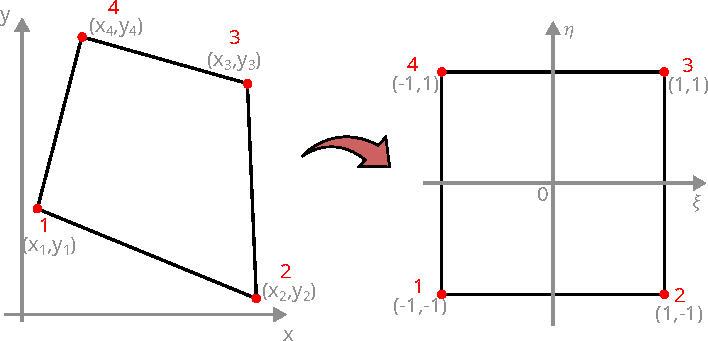
\includegraphics[scale=1]{Figures/9-Isoparametrico/Quadrado.pdf}
            \caption{Mapeamento entre um elemento quadrangular qualquer para um quadrado regular}
            \label{fig:elemento_quadrado}
        \end{figure}

        Para construir as funções de forma deste elemento, construímos funções de forma com polinômios de Lagrange (Seção \ref{sec:lagrange}):

        \begin{equation*}
            f_1(\xi) = \frac{1}{2}\left(1-\xi\right) \quad \quad f_1(\eta) = \frac{1}{2}\left(1-\eta\right)
        \end{equation*}

        \begin{equation*}
            f_2(\xi) = \frac{1}{2}\left(1+\xi\right) \quad \quad f_2(\eta) = \frac{1}{2}\left(1+\eta\right)
        \end{equation*}

        As funções de forma deste elemento são montadas multiplicando cada combinação dessas funções. Estas funções mantêm a propriedade dos polinômios de Lagrange de apenas uma ser unitária em cada nó e as outras serem nulas:

        \begin{equation}
            \begin{array}{l}
                N_1(\xi, \eta) = f_1(\xi)f_1(\eta) = \frac{1}{4}\left(1-\xi\right)\left(1-\eta\right)\\
                N_2(\xi, \eta) = f_2(\xi)f_1(\eta) = \frac{1}{4}\left(1+\xi\right)\left(1-\eta\right)\\
                N_3(\xi, \eta) = f_2(\xi)f_2(\eta) = \frac{1}{4}\left(1+\xi\right)\left(1+\eta\right)\\
                N_4(\xi, \eta) = f_1(\xi)f_2(\eta) = \frac{1}{4}\left(1-\xi\right)\left(1+\eta\right)\\
            \end{array}
        \end{equation}

        Ao definir as funções de forma de um elemento, é importante manter a consistência entre a numeração dos nós. No caso do elemento quadrado, numeramos os nós em sentido anti-horário (Figura \ref{fig:elemento_quadrado}). Finalmente, este elemento é normalmente dito como bilinear, visto que suas funções são lineares em cada variável $\xi$ e $\eta$, mas não são lineares, pois incluem o termo cruzado $\xi \eta$.

        As derivadas dessas funções de forma, em relação às coordenadas locais são:

        \begin{equation*}
            \frac{\partial N_1}{\partial \xi} = -\frac{1}{4}\left(1-\eta\right)  \quad \quad 
            \frac{\partial N_1}{\partial \eta} = -\frac{1}{4}\left(1-\xi\right)
        \end{equation*}

        \begin{equation*}
            \frac{\partial N_2}{\partial \xi} = \frac{1}{4}\left(1-\eta\right)  \quad \quad 
            \frac{\partial N_2}{\partial \eta} = -\frac{1}{4}\left(1+\xi\right)
        \end{equation*}

        \begin{equation*}
            \frac{\partial N_3}{\partial \xi} = \frac{1}{4}\left(1+\eta\right)  \quad \quad 
            \frac{\partial N_3}{\partial \eta} = \frac{1}{4}\left(1+\xi\right)
        \end{equation*}

        \begin{equation}
            \frac{\partial N_4}{\partial \xi} = -\frac{1}{4}\left(1+\eta\right)  \quad \quad 
            \frac{\partial N_4}{\partial \eta} = \frac{1}{4}\left(1-\xi\right)
        \end{equation}


        A relação entre as coordenadas locais e global é:

        \begin{equation*}
            x(\xi, \eta) = \sum N_i(\xi,\eta) x_i
        \end{equation*}

        \begin{equation}
            y(\xi, \eta) = \sum N_i(\xi,\eta) y_i
        \end{equation}

        As derivadas, em relação às coordenadas locais, são:

        \begin{equation*}
            \frac{\partial x}{\partial \xi} = \left(x_1-x_2+x_3-x_4\right)\eta + \left(-x_1+x_2+x_3-x_4\right)
        \end{equation*}

        \begin{equation*}
            \frac{\partial x}{\partial \eta} = \left(x_1-x_2+x_3-x_4\right)\xi + \left(-x_1-x_2+x_3+x_4\right)
        \end{equation*}

        \begin{equation*}
            \frac{\partial y}{\partial \xi} = \left(y_1-y_2+y_3-y_4\right)\eta + \left(-y_1+y_2+y_3-y_4\right)
        \end{equation*}

        \begin{equation*}
            \frac{\partial y}{\partial \eta} = \left(y_1-y_2+y_3-y_4\right)\xi + \left(-y_1-y_2+y_3+y_4\right)
        \end{equation*}

        Com isso, temos a matriz Jacobiana:

        \begin{equation}
            \mathbf{J}(\xi, \eta) = 
            \begin{bmatrix}
                 \frac{\partial x}{\partial \xi} &  \frac{\partial y}{\partial \xi}\\
                 \frac{\partial x}{\partial \eta} &  \frac{\partial y}{\partial \eta}
            \end{bmatrix}
        \end{equation}

        \noindent note que, neste caso, o Jacobiano não necessariamente será constante. Consequentemente, seu determinante também não será constante.

        As derivadas das funções de forma em relação às coordenadas globais são obtidas como na Seção \ref{sec:elemento_triangular}:

        \begin{equation}
            \begin{Bmatrix}
                \frac{\partial N_i}{\partial x} \\
                \frac{\partial N_i}{\partial y}
            \end{Bmatrix} = 
            \mathbf{J}^{-1}
            \begin{Bmatrix}
                \frac{\partial N_i}{\partial \xi} \\
                \frac{\partial N_i}{\partial \eta}
            \end{Bmatrix}
        \end{equation}

        Com as derivadas, podemos montar a matriz $\mathbf{B}$ do elemento. Por exemplo, no elemento de estado plano (Seção \ref{sec:estado_plano}):

        \begin{equation}
            \mathbf{B} = 
            \begin{bmatrix}
                \frac{\partial N_1}{\partial x} & 0 & \cdots & \frac{\partial N_n}{\partial x} & 0\\
                0 & \frac{\partial N_1}{\partial y} & \cdots & 0 & \frac{\partial N_n}{\partial y}\\
                \frac{\partial N_1}{\partial y} & \frac{\partial N_1}{\partial x} & \cdots & \frac{\partial N_n}{\partial y} & \frac{\partial N_n}{\partial x}\\
            \end{bmatrix}
        \end{equation}

        Com isso, podemos encontrar a matriz de rigidez de um elemento resolvendo a integral:

        \begin{equation}
            \mathbf{K}_e = \int_\Omega  \mathbf{B}^T \mathbf{D} \mathbf{B} dA
        \end{equation}

        Aplicando uma mudança de variáveis:

        \begin{equation}
            \mathbf{K}_e = \int_{-1}^{1} \int_{-1}^{1}  \mathbf{B}^T \mathbf{D} \mathbf{B} \det \mathbf{J} d\xi d\eta
        \end{equation}


    \subsection{Elemento hexaédrico isoparamétrico}

        Da mesma forma que a construção de um elemento quadrangular é feita pela multiplicação de funções de forma unidimensionais, para um elemento hexaédrico (Figura \ref{fig:elemento_cubo}), isto é feito de forma similar:

        \begin{figure}[h!]
            \centering
            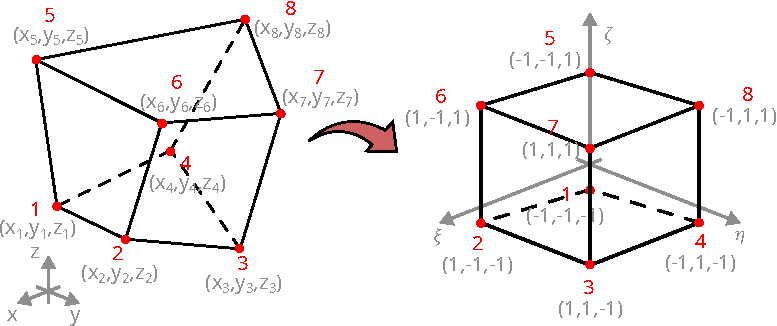
\includegraphics[scale=1]{Figures/9-Isoparametrico/Hexaedro.pdf}
            \caption{Mapeamento entre um elemento hexaédrico qualquer para um cubo regular}
            \label{fig:elemento_cubo}
        \end{figure}

        \begin{equation}
            \begin{array}{l}
                N_1(\xi, \eta, \zeta) = f_1(\xi)f_1(\eta)f_1(\zeta) = \frac{1}{8}\left(1-\xi\right)\left(1-\eta\right)\left(1-\zeta\right)\\
                N_2(\xi, \eta, \zeta) = f_2(\xi)f_1(\eta)f_1(\zeta) = \frac{1}{8}\left(1+\xi\right)\left(1-\eta\right)\left(1-\zeta\right)\\
                N_3(\xi, \eta, \zeta) = f_2(\xi)f_2(\eta)f_1(\zeta) = \frac{1}{8}\left(1+\xi\right)\left(1+\eta\right)\left(1-\zeta\right)\\
                N_4(\xi, \eta, \zeta) = f_1(\xi)f_2(\eta)f_1(\zeta) = \frac{1}{8}\left(1-\xi\right)\left(1+\eta\right)\left(1-\zeta\right)\\
                N_5(\xi, \eta, \zeta) = f_1(\xi)f_1(\eta)f_2(\zeta) = \frac{1}{8}\left(1-\xi\right)\left(1-\eta\right)\left(1+\zeta\right)\\
                N_6(\xi, \eta, \zeta) = f_2(\xi)f_1(\eta)f_2(\zeta) = \frac{1}{8}\left(1+\xi\right)\left(1-\eta\right)\left(1+\zeta\right)\\
                N_7(\xi, \eta, \zeta) = f_2(\xi)f_2(\eta)f_2(\zeta) = \frac{1}{8}\left(1+\xi\right)\left(1+\eta\right)\left(1+\zeta\right)\\
                N_8(\xi, \eta, \zeta) = f_1(\xi)f_2(\eta)f_2(\zeta) = \frac{1}{8}\left(1-\xi\right)\left(1+\eta\right)\left(1+\zeta\right)\\
            \end{array}
        \end{equation}
    
        Suas derivadas são:

        \begin{equation*}
            \frac{\partial N_1}{\partial \xi} = -\frac{1}{8}\left(1-\eta\right)\left(1-\zeta\right)  \quad \quad 
            \frac{\partial N_1}{\partial \eta} = -\frac{1}{8}\left(1-\xi\right)\left(1-\zeta\right)  \quad \quad 
            \frac{\partial N_1}{\partial \zeta} = -\frac{1}{8}\left(1-\xi\right)\left(1-\eta\right)
        \end{equation*}

        \begin{equation*}
            \frac{\partial N_2}{\partial \xi} =  \frac{1}{8}\left(1-\eta\right)\left(1-\zeta\right)  \quad \quad 
            \frac{\partial N_2}{\partial \eta} = -\frac{1}{8}\left(1+\xi\right)\left(1-\zeta\right)  \quad \quad 
            \frac{\partial N_2}{\partial \zeta} = -\frac{1}{8}\left(1+\xi\right)\left(1-\eta\right)
        \end{equation*}

        \begin{equation*}
            \frac{\partial N_3}{\partial \xi} =  \frac{1}{8}\left(1+\eta\right)\left(1-\zeta\right)  \quad \quad 
            \frac{\partial N_3}{\partial \eta} =  \frac{1}{8}\left(1+\xi\right)\left(1-\zeta\right)  \quad \quad 
            \frac{\partial N_3}{\partial \zeta} = -\frac{1}{8}\left(1+\xi\right)\left(1+\eta\right)
        \end{equation*}

        \begin{equation*}
            \frac{\partial N_4}{\partial \xi} = -\frac{1}{8}\left(1+\eta\right)\left(1-\zeta\right)  \quad \quad 
            \frac{\partial N_4}{\partial \eta} =  \frac{1}{8}\left(1-\xi\right)\left(1-\zeta\right)  \quad \quad 
            \frac{\partial N_4}{\partial \zeta} = -\frac{1}{8}\left(1-\xi\right)\left(1+\eta\right)
        \end{equation*}

        \begin{equation*}
            \frac{\partial N_5}{\partial \xi} = -\frac{1}{8}\left(1-\eta\right)\left(1+\zeta\right)  \quad \quad 
            \frac{\partial N_5}{\partial \eta} = -\frac{1}{8}\left(1-\xi\right)\left(1+\zeta\right)  \quad \quad 
            \frac{\partial N_5}{\partial \zeta} =  \frac{1}{8}\left(1-\xi\right)\left(1-\eta\right)
        \end{equation*}

        \begin{equation*}
            \frac{\partial N_6}{\partial \xi} =  \frac{1}{8}\left(1-\eta\right)\left(1+\zeta\right)  \quad \quad 
            \frac{\partial N_6}{\partial \eta} = -\frac{1}{8}\left(1+\xi\right)\left(1+\zeta\right)  \quad \quad 
            \frac{\partial N_6}{\partial \zeta} =  \frac{1}{8}\left(1+\xi\right)\left(1-\eta\right)
        \end{equation*}

        \begin{equation*}
            \frac{\partial N_7}{\partial \xi} =  \frac{1}{8}\left(1+\eta\right)\left(1+\zeta\right)  \quad \quad 
            \frac{\partial N_7}{\partial \eta} =  \frac{1}{8}\left(1+\xi\right)\left(1+\zeta\right)  \quad \quad 
            \frac{\partial N_7}{\partial \zeta} =  \frac{1}{8}\left(1+\xi\right)\left(1+\eta\right)
        \end{equation*}

        \begin{equation}
            \frac{\partial N_8}{\partial \xi} = -\frac{1}{8}\left(1+\eta\right)\left(1+\zeta\right)  \quad \quad 
            \frac{\partial N_8}{\partial \eta} =  \frac{1}{8}\left(1-\xi\right)\left(1+\zeta\right)  \quad \quad 
            \frac{\partial N_8}{\partial \zeta} =  \frac{1}{8}\left(1-\xi\right)\left(1+\eta\right)
        \end{equation}

        A relação entre as coordenadas locais e global é:

        \begin{equation*}
            x(\xi, \eta, \zeta) = \sum N_i(\xi,\eta, \zeta) x_i
        \end{equation*}

        \begin{equation*}
            y(\xi, \eta, \zeta) = \sum N_i(\xi,\eta,\zeta) y_i
        \end{equation*}

        \begin{equation}
            z(\xi, \eta, \zeta) = \sum N_i(\xi,\eta,\zeta) z_i
        \end{equation}


        Com as derivadas das coordenadas em relação as coordenadas locais, temos a matriz Jacobiana:

        \begin{equation}
            \mathbf{J}(\xi, \eta, \zeta) = 
            \begin{bmatrix}
                \frac{\partial x}{\partial \xi} &  \frac{\partial y}{\partial \xi} &  \frac{\partial z}{\partial \xi}\\
                \frac{\partial x}{\partial \eta} &  \frac{\partial y}{\partial \eta} &  \frac{\partial z}{\partial \eta}\\
                \frac{\partial x}{\partial \zeta} &  \frac{\partial y}{\partial \zeta} &  \frac{\partial z}{\partial \zeta}
            \end{bmatrix}
        \end{equation}

        \noindent novamente, o Jacobiano não será constante. Consequentemente, seu determinante também não será constante.


        As derivadas das funções de forma em relação às coordenadas globais são obtidas como anteriormente:

        \begin{equation}
            \begin{Bmatrix}
                \frac{\partial N_i}{\partial x} \\
                \frac{\partial N_i}{\partial y} \\
                \frac{\partial N_i}{\partial z}
            \end{Bmatrix} = 
            \mathbf{J}^{-1}
            \begin{Bmatrix}
                \frac{\partial N_i}{\partial \xi} \\
                \frac{\partial N_i}{\partial \eta} \\
                \frac{\partial N_i}{\partial \zeta}
            \end{Bmatrix}
        \end{equation}

        Com as derivadas, podemos montar a matriz $\mathbf{B}$ do elemento. Nesta apostila, não será feita a dedução para o caso de elasticidade geral, mas ela é similar ao da Seção \ref{sec:estado_plano}:

        \begin{equation}
            \mathbf{B} = 
            \begin{bmatrix}
                \frac{\partial N_1}{\partial x} & 0 & 0 & \cdots & \frac{\partial N_n}{\partial x} & 0 & 0\\
                0 & \frac{\partial N_1}{\partial y} & 0 & \cdots & 0 & \frac{\partial N_n}{\partial y} & 0\\
                0 & 0 & \frac{\partial N_1}{\partial z} & \cdots & 0 & 0 & \frac{\partial N_n}{\partial z} \\
                \frac{\partial N_1}{\partial y} & \frac{\partial N_1}{\partial x} & 0 & \cdots & \frac{\partial N_n}{\partial y} & \frac{\partial N_n}{\partial x} & 0\\
                \frac{\partial N_1}{\partial z} & 0 & \frac{\partial N_1}{\partial x} & \cdots & \frac{\partial N_n}{\partial z} & 0 & \frac{\partial N_n}{\partial x}\\
                0 & \frac{\partial N_1}{\partial z} & \frac{\partial N_1}{\partial y} & \cdots & 0 & \frac{\partial N_n}{\partial z} & \frac{\partial N_n}{\partial y}\\
            \end{bmatrix}
        \end{equation}

        Para um material linear elástico isotrópico, temos a matriz constitutiva também:

        \begin{equation}
            \mathbf{D} =
            \frac{E}{\left(1+\nu\right)\left(1-2\nu\right)}
            \begin{bmatrix}
                1-\nu & \nu & \nu & 0 & 0 & 0\\
                \nu & 1-\nu & \nu & 0 & 0 & 0\\
                \nu & \nu & 1-\nu & 0 & 0 & 0\\
                0 & 0 & 0 & \frac{1-2\nu}{2} & 0 & 0\\
                0 & 0 & 0 & 0 & \frac{1-2\nu}{2} & 0\\
                0 & 0 & 0 & 0 & 0 & \frac{1-2\nu}{2}
            \end{bmatrix}
        \end{equation}

        Com isso, podemos encontrar a matriz de rigidez de um elemento resolvendo a integral:

        \begin{equation}
            \mathbf{K}_e = \int_\Omega  \mathbf{B}^T \mathbf{D} \mathbf{B} dV
        \end{equation}

        Aplicando uma mudança de variáveis:

        \begin{equation}
            \mathbf{K}_e = \int_{-1}^{1} \int_{-1}^{1} \int_{-1}^{1}  \mathbf{B}^T \mathbf{D} \mathbf{B} \det \mathbf{J} d\xi d\eta d\zeta
        \end{equation}



    \subsection{Integração no domínio 2D e 3D}
    \label{sec:integracaonD}

        Para integrar as matrizes dos elementos quadrangulares e hexaédricos, será utilizado o procedimento de integração por quadratura de Gauss-Legendre, conforme apresentado na Seção \ref{sec:integracao1D}.

        Considere uma função de duas ou de três variáveis, que devem ser integradas entre os limites $-1$ e $1$ para cada uma dessas. A integral será aproximada por:

        \begin{equation*}
            \int_{-1}^{1} \int_{-1}^{1} f(\xi, \eta) d\xi d\eta \approx 
            \sum\limits_{p=1}^{n_p} f(\xi_p,\eta_p) w_p = 
            \sum\limits_{i=1}^{n_1} \sum\limits_{j=1}^{n_2} f(\xi_i,\eta_j) w_i^{(\xi)} w_j^{(\eta)}
        \end{equation*}

        \begin{equation*}
            \int_{-1}^{1} \int_{-1}^{1} \int_{-1}^{1} f(\xi, \eta, \zeta) d\xi d\eta d\zeta \approx 
            \sum\limits_{p=1}^{n_p} f(\xi_p,\eta_p, \zeta_p) w_p = 
            \sum\limits_{i=1}^{n_1} \sum\limits_{j=1}^{n_2} \sum\limits_{k=1}^{n_3} f(\xi_i,\eta_j, \zeta_k) w_i^{(\xi)} w_j^{(\eta)} w_k^{(\zeta)}
        \end{equation*}

        Para encontrar os pontos de integração e os pesos, podemos considerar variável a variável. Isto é, consideramos apenas o procedimento de integração para uma função de uma variável $\xi$. Determinamos os pontos de integração e pesos $\xi_i, w_i^{(\xi)}$, baseado no grau do polinômio integrado em $\xi$. Em seguida, fazemos o mesmo para $\eta$ e $\zeta$. Finalmente, fazemos uma combinação dos pontos obtidos para cada variável (Figura \ref{fig:integracao_2d}). Portanto, se temos, por exemplo, em um caso 2D, 2 pontos para $\xi$ e 2 para $\eta$, teremos, no final, 4 pontos de integração.

        \begin{figure}[h!]
            \centering
            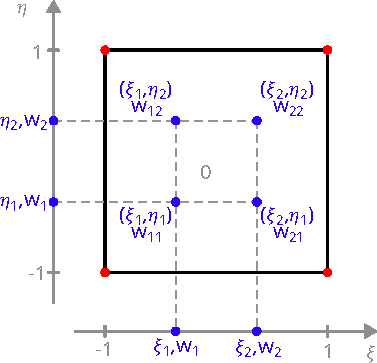
\includegraphics[scale=1.5]{Figures/9-Isoparametrico/Integracao.pdf}
            \caption{Integração em dimensões maiores a partir de uma dimensão}
            \label{fig:integracao_2d}
        \end{figure}

        Para elementos triangulares ou tetraédricos, o procedimento para obter os pontos de integração não é tão simples, visto que as integrais não têm limites constantes. Para este tipo de elemento, com funções de forma lineares, os termos da matriz de rigidez ficam constantes. Portanto, não é necessária uma integração numérica. Entretanto, se aumentamos a ordem dos elementos, ela se torna necessária; ou se integrarmos uma força mais complexa. Existem propostas para obter os pontos de integração desses elementos; entretanto, na prática, são usadas tabelas com os pontos de integração.

        \subsubsection{Exemplo}

        Resolva a integral abaixo usando integração de Gauss-Legendre:

        \begin{equation*}
            \int_{0}^{2} \int_{0}^{1} \left(x^2y + xy^2  \right) dx dy
        \end{equation*}

        \subsubsection*{Solução}

        A integral analítica pode ser obtida como:

        \begin{equation*}
            \int_{0}^{2} \int_{0}^{1} (x^2y + xy^2) dx dy = 
            \int_{0}^{2} \left[\frac{x^3}{3}y + \frac{x^2}{2}y^2\right]_0^1 dy
        \end{equation*}

        \begin{equation*}
            \int_{0}^{2} \frac{y}{3} + \frac{y^2}{2} dy = 
            \left[\frac{y^2}{6} + \frac{y^3}{6}\right]_0^2 = \frac{4}{6} + \frac{8}{6} = 2
        \end{equation*}

        Para integrar numericamente, precisamos fazer um mapeamento entre as coordenadas $x$ e $y$ para coordenadas locais $\xi$ e $\eta$, cujos limites de integração são $-1$ e $1$. No caso, $x$ apenas depende de $\xi$, e $y$, apenas de $\eta$:

        \begin{equation*}
            x(\xi) = \frac{1}{2}(1+\xi)
        \end{equation*}

        \begin{equation*}
            y(\eta) = 1+\eta
        \end{equation*}

        \begin{equation*}
            \frac{dx}{d\xi} = \frac{1}{2}
        \end{equation*}

        \begin{equation*}
            \frac{dy}{d\eta} = 1
        \end{equation*}

        O Jacobiano e seu determinante são:

        \begin{equation*}
            \mathbf{J} = 
            \begin{bmatrix}
                 \frac{\partial x}{\partial \xi} &  \frac{\partial y}{\partial \xi}\\
                 \frac{\partial x}{\partial \eta} &  \frac{\partial y}{\partial \eta}
            \end{bmatrix} =
            \begin{bmatrix}
                \frac{1}{2} & 0\\
                0 & 1
            \end{bmatrix}
        \end{equation*}

        \begin{equation*}
            \det \mathbf{J} = 
            \frac{1}{2}
        \end{equation*}

        \begin{equation*}
            \int_{0}^{2} \int_{0}^{1} (x^2y + xy^2) dx dy = 
            \int_{-1}^{1} \int_{-1}^{1} (x(\xi)^2y(\eta) + x(\xi)y(\eta)^2) \det \mathbf{J} d\xi d\eta 
        \end{equation*}

        Como são funções polinomiais em $\xi$ e $\eta$, podemos encontrar um número mínimo de pontos de Gauss tal que a integração seja exata:

        \begin{equation*}
            N_\xi \geq \frac{P_\xi+1}{2} = \frac{2+1}{2} = 1,5
        \end{equation*}

        \begin{equation*}
            N_\eta \geq \frac{P_\xi+1}{2} = \frac{2+1}{2} = 1,5
        \end{equation*}

        Finalmente, calculamos a integral para dois números de pontos de Gauss para verificar:

        \begin{equation*}
            n_x \times n_y =  1 \times 1 \rightarrow \int_{0}^{2} \int_{0}^{1} (x^2y + xy^2) dx dy \approx  1,5\rightarrow \text{erro de } 25\% 
        \end{equation*}

        \begin{equation*}
            n_x \times n_y =  2 \times 2 \rightarrow \int_{0}^{2} \int_{0}^{1} (x^2y + xy^2) dx dy =  2 \rightarrow \text{erro de } 0\% 
        \end{equation*}


	%LTeX: language=pt-br
% !TeX root = Apostila_IM381.tex

\cleardoublepage
\section{Considerações e propriedades}

    Nesta seção, serão discutidas algumas fontes de erros no Método de Elementos Finitos, assim como algumas considerações adicionais que devem ser levadas em conta ao realizar a análise numérica.

    Conforme apresentado nas seções anteriores, o MEF é um método numérico no qual obtemos uma solução aproximada do problema analisado. Desta forma, erros aparecem na solução. Há várias fontes de erro que podem poluir o resultado, e conhecê-las nos auxilia na interpretação dos valores obtidos. Conhecê-las também nos permite ter uma confiabilidade maior no método, assim como diagnosticar as causas de erros nos resultados.

    Em problemas complexos, sem solução analítica bem definida, não há nenhuma garantia de solução exata. Na verdade, nestes casos, espera-se que nunca cheguemos precisamente na solução exata, erros sempre estarão inclusos no nosso resultado. Estes podem ser dividos nas seguintes categorias:

    \subsubsection*{Erros de modelagem}

        Antes de aplicar o MEF, precisamos de um modelo matemático representativo do sistema. Estes erros provêm da diferença entre o comportamento real e o modelo matemático adotado.

        Por exemplo, um modelo de material linear elástico isotrópico e homogêneo será representativo para um aço. Entretanto, a depender do tratamento térmico, pode ser que este material perca sua isotropia, e o modelo deixe de representar adequadamente o sistema real. Um polímero também terá erros consideráveis se utilizarmos este modelo, exigindo a aplicação de modelos constitutivos de materiais hiperelásticos.

        

        Outros exemplos de erros de modelagem que se inserem aqui são: aplicação indevida de modelos de pequenas deformações ou pequenos deslocamentos, imprecisões nas aproximações das condições de contorno do sistema. Representação aproximada das cargas impostas no sistema.

        Para corrigir estes erros, é necessário que o engenheiro tenha a capacidade de discernimento sobre o quão adequado é cada modelo para aquela aplicação específica, visto que modelos mais complexos exigem um maior custo computacional.

    \subsubsection*{Erros de discretização}

        Conforme estudado nas seções anteriores, o MEF é um método numérico no qual obtemos uma solução aproximada para a função incógnita. Esta pode ser um campo de temperatura, campo de potencial elétrico, campo de deslocamentos, entre outros.

        Esta função incógnita pertence a um espaço $V$ de dimensão infinita. A priori, deconhecemos quem deve ser esta função solução, inclusive, está pode nem ser análitica, basta que ela pertença a $V$. O MEF aproxima a solução para um espaço de dimensão finita $V^h$, obtendo a função deste espaço que melhor se aproxima da exata.

        Os erros de discretização provêm da diferença entre a solução exata e a solução aproximada obtida. Em casos particulares, como barras, eixos, vigas e placas, é possível que esta diferença seja zero. Entretanto, de forma geral, sempre haverá um erro, não importa o quanto aumentemos a dimensão de $V^h$, isto é, não importa o quanto aumentemos o número de funções de forma, refinando a malha em mais elementos finitos. A Figura \ref{fig:discretizacao_erro} ilustra este erro, mostrando a diferença entre as deformações e deslocamentos de um problema de barra.

        \begin{figure}[h!]
            \begin{subfigure}{0.9\textwidth}
                \centering
                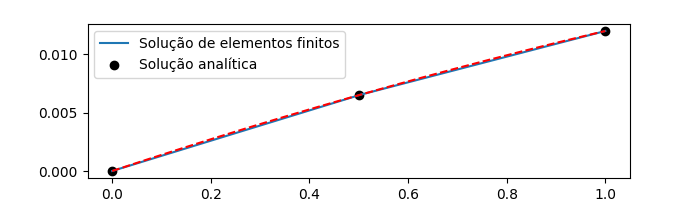
\includegraphics[scale=0.9]{Figures/4-Elemento_barra/Deslocamento_exemplo_4-1.png}
                \caption{}
            \end{subfigure}\\
            \begin{subfigure}{0.9\textwidth}
                \centering
                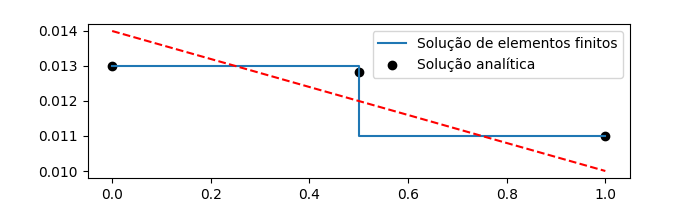
\includegraphics[scale=0.9]{Figures/4-Elemento_barra/Deformacao_exemplo_4-1.png}
                \caption{}
            \end{subfigure}
            \caption{Erros de discretização em barra. (a) Deslocamento, (b) deformação}
            \label{fig:discretizacao_erro}
        \end{figure}

        Este erro também inclui imprecisões sobre a geometria do domínio, como mostrado na Figura \ref{fig:modelo_erro}. Muitas vezes, os elementos adotados não se encaixam perfeitamente na geometria, e a superfície do modelo passa a ser uma aproximação da geometria real.

        \begin{figure}[h!]
            \centering
            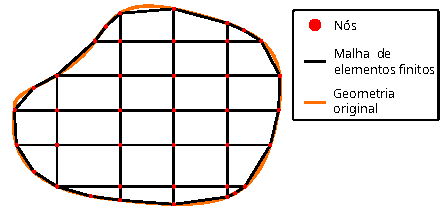
\includegraphics[scale=1]{Figures/4-Elemento_barra/Malha.pdf}
            \caption{Discretização de uma geometria em elementos finitos}
            \label{fig:modelo_erro}
        \end{figure}

    \subsubsection*{Erros de truncamento}

    Um computador salva os números como variáveis que ocupam certas estruturas específicas. Por exemplo, um valor pode ser salvo como uma variável inteira \textit{int} ou \textit{long}. Ambos salvam variáveis inteiras, porém, a diferença entre elas é a sua precisão, isto é, o tamanho dos números que estas são capazes de armazenar. Para armazenar variáveis com uma precisão superior, é necessário utilizar um espaço maior da memória.

    Para variáveis reais, de forma geral, utiliza-se o tipo \textit{float} ou \textit{double}. Nas linguagens C/C++, a primeira utiliza 4 bytes de memória para armazenar por volta de 7 algarismos significativos, a segunda ocupa 8 bytes e armazena por volta de 15 algarismos. No Python, o tipo chamado \textit{float} na verdade corresponde ao \textit{double} da linguagem C.

    As variáveis \textit{float} e \textit{double} aloca números sempre em notação científica em base binária. Nesta notação, qualquer número será da seguinte forma:

    \begin{equation}
        \textit{num. binário em notação científica} = 1, \square \times 10^\square
    \end{equation}

    Por exemplo:

    \begin{equation*}
        65.25 = 1000001.01 = 1.00000101 \times 10^6
    \end{equation*}

    \begin{equation*}
        -0.171875 = -0.001011 = -1.011 \times 10^{-3}
    \end{equation*}

    Portanto, devem ser salvas três informações: o sinal, o expoente e a mantissa (dígitos que aparecem após a vírgula).

    Um \textit{double} possui 8 bytes, isto é, 64 bits (lembrando que 1 byte possui 8 bits). Um bit é a unidade de armazenamento em um computador, e armazena um dado de forma binária, isto é, pode estar ativado (1) ou desativado (0). O sinal é armazenado em 1 bit, representando positivo ou negativo. O expoente é representado em 11 bits, e a mantissa nos últimos 52 bits. Caso o número seja irracional ou uma dízima periódica (na base binária!), então este será truncado e representado de forma aproximada na memória.

     \begin{lstlisting}[language=C++]
        /**
            Exemplo de erros devido a precisao numerica
            em codigo em C
        **/

        // Pi salvo em float
        float pi_float = 3.1415927;

        // Pi salvo em double
        double pi_double = 3.141592653589793;

    \end{lstlisting}

    \subsubsection*{Erros de manipulação numérica}

    Ainda no contexto do erro de truncamento, como as variáveis são truncadas, podem aparecer erros em determinadas operações devido a este truncamento:

    \begin{lstlisting}[language=Python]
        # Exemplo de erros em Python

        print(2.1 * 7)
        # >> 14.700000000000001
        # 2.1 em binario: 10.0001100110011001101
        # Dizima periodica em binario!

        print(1.000000000000001 - 1)
        # >> 1.1102230246251565e-15
        
        print(1 + 1e-16 - 1)
        # >> 0.0

    \end{lstlisting}

    Principalmente em operações que devem ser muito próximas de zero, pode aparecer um erro significativo na resposta. Se, por sua vez, este valor estiver, por exemplo, no denominador de uma divisão, isso pode levar a uma explosão no erro numérico associado a essa operação. Por esta causa, normalmente os métodos numéricos evitam operar com divisões de números pequenos. Um exemplo disso é na solução de sistemas lineares, no qual é feita uma permutação na etapa de pivotamento, para reduzir este tipo de erro.

    Além disso, podemos perder informação significativa para o resultado se somarmos ou subtrairmos dois números com ordens de grandeza muito distintas:

    \begin{lstlisting}[language=Python]
        # Exemplo de erros em Python

        print(1 + 1e-16 - 1)
        # >> 0.0

        print(1 -1 + 1e-16)
        # >> 1e-16

        print(1.000000000000001 -1 + 1e-16)
        # >> 1.2102230246251566e-15

    \end{lstlisting}

    Portanto, também evita-se operar números com esta característica. Se possível, podemos alterar a ordem das operações para reduzir erros, entretanto, esta troca ainda pode trazer os erros citados acima.



    \subsection{Condicionamento de uma matriz}

        No MEF, obtemos uma matriz, chamada matriz de rigidez. Esta matriz, junto com o vetor de forças, resulta no campo de deslocamentos nodais. Desta forma, a matriz de rigidez carrega toda a informação do problema analisado. Portanto, é essencial garantir que esta matriz carregue adequadamente estas informações. Para isso, usaremos algumas propriedades da Álgebra Linear.

        Uma matriz, no contexto do espaço vetorial dos vetores euclidianos, é um tensor. Isto é, ela representa uma transformação linear aplicada a um vetor. A Figura \ref{fig:transformacao_linear} ilustra essa operação. O vetor $\bm{u}$ sofre uma transformação linear pela aplicação do tensor $\bm{T}$, resultando no vetor $\bm{v}$. Matematicamente:

        \begin{equation}
            \bm{v} = \bm{T} \bm{u}
        \end{equation}

        \begin{figure}[h!]
            \centering
            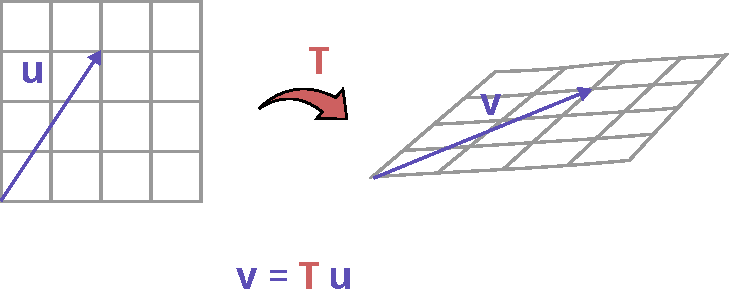
\includegraphics[scale=1]{Figures/10-Consideracoes/Matriz.pdf}
            \caption{Aplicação de uma transformação linear. O espaço se distorce após está, e o vetor muda de direção e módulo.}
            \label{fig:transformacao_linear}
        \end{figure}

        O condicionamento de uma matriz mede o quão sensível o vetor resultante $\bm{v}$ é à uma perturbação no vetor inicial $\bm{u}$. Uma matriz é dita bem condicionada se ele é pouco sensível. Em uma matriz mal condicionada, a solução é bastante sensível a pequenas perturbações. A Figura \ref{fig:mal_condicionado} ilustra uma transformação descrita por uma matriz mal condicionada.

        \begin{figure}[h!]
            \centering
            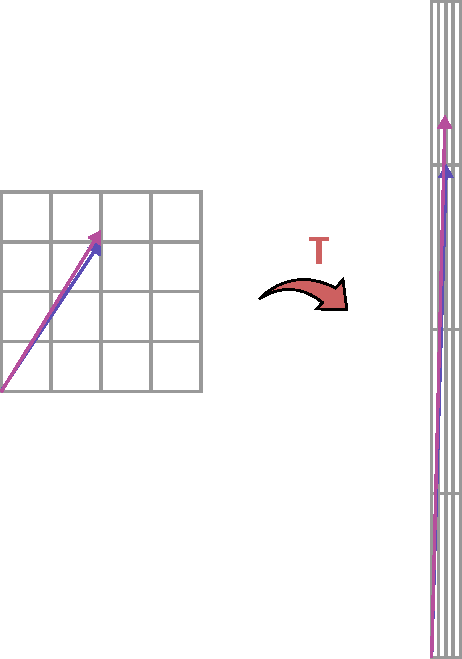
\includegraphics[scale=1]{Figures/10-Consideracoes/Matriz_condicionamento.pdf}
            \caption{Aplicação de uma transformação linear mal condicionada.}
            \label{fig:mal_condicionado}
        \end{figure}

        Um sistema linear representado por uma matriz mal condicionada apresenta uma sensibilidade maior a perturbações nos valores da matriz.

        Vamos verificar essa sensibilidade com um exemplo, abaixo:

        \begin{equation}
            \begin{bmatrix}
                1 & -1\\
                -1 & 1+a
            \end{bmatrix}
            \begin{Bmatrix}
                x_1\\
                x_2
            \end{Bmatrix}
            =
            \begin{Bmatrix}
                4\\
                -2
            \end{Bmatrix}
        \end{equation}

        Se resolvermos este sistema, chegamos a seguinte solução:

        \begin{equation}
            \begin{Bmatrix}
                x_1\\
                x_2
            \end{Bmatrix}
            =
            \begin{Bmatrix}
                4+\frac{2}{a}\\
                \frac{2}{a}
            \end{Bmatrix}
        \end{equation}

        Vamos agora adotar valores para $a$ para observar 

        \begin{equation}
            a =0,01
            \rightarrow
            \begin{Bmatrix}
                x_1\\
                x_2
            \end{Bmatrix}
            =
            \begin{Bmatrix}
                204\\
                200
            \end{Bmatrix}
        \end{equation}

        \begin{equation}
            a =0,009
            \rightarrow
            \begin{Bmatrix}
                x_1\\
                x_2
            \end{Bmatrix}
            =
            \begin{Bmatrix}
                226,2\\
                222,2
            \end{Bmatrix}
        \end{equation}

        Uma pequena variação no valor de $a$ resultou em uma diferença expressiva na resposta. Perceba que esta diferença representa uma mudança de $1,01$ para $1,009$ no termo da matriz, uma variação de menos de 1\% no valor.

        Na prática, em problemas computacionais, conforme mostrado anteriormente, teremos erros de truncamento associados às operações de máquina. Visto a inevitabilidade desses erros, desejamos matrizes bem condicionadas, para evitar que estes sejam amplificados demasiadamente.

        \subsubsection*{Exemplo: molas em série}

            Para ilustrar o efeito do mau condicionamento de uma matriz, considere o sistema da Figura \ref{fig:molas}, composto por duas molas em série, com rigidezes $k_1$ e $k_2$. A mola de rigidez $k_2$ está presa em uma parede fixa, a outra está sujeita a uma força $F$. A equação de equilíbrio deste sistema é dado por:

            \begin{equation}
                \begin{bmatrix}
                    k_1 & -k_1\\
                    -k_1 & k_1 + k_2
                \end{bmatrix}
                \begin{Bmatrix}
                    u_1\\
                    u_2
                \end{Bmatrix}
                =
                \begin{Bmatrix}
                    F\\
                    0
                \end{Bmatrix}
            \end{equation}

            \begin{figure}[h!]
                \centering
                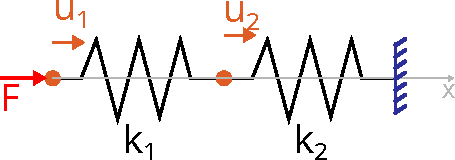
\includegraphics[scale=1]{Figures/10-Consideracoes/Molas.pdf}
                \caption{Molas em série}
                \label{fig:molas}
            \end{figure}

            Resolvendo este sistema, chegamos nos deslocamentos:

            \begin{equation}
                u_1 = \frac{F}{k_1} + \frac{F}{k_2} \quad , \quad  u_2 = \frac{F}{k_2}
            \end{equation}

            Suponha agora, que $k_2 \gg k_1$. Quando realizamos a operação $k_1 + k_2$, se o segundo for muito maior que o primeiro, devido à precisão de máquina, teremos apenas $k_1 + k_2 \approx k_2$:

            \begin{equation}
                \begin{bmatrix}
                    k_1 & -k_1\\
                    -k_1 & k_2
                \end{bmatrix}
                \begin{Bmatrix}
                    u_1\\
                    u_2
                \end{Bmatrix}
                =
                \begin{Bmatrix}
                    F\\
                    0
                \end{Bmatrix}
            \end{equation}

            Este sistema será resolvido normalmente, resultando em:

            \begin{equation}
                u_1 \approx \frac{F}{k_1} + \frac{F}{k_2} \quad , \quad  
                u_2 = \frac{F}{k_2-k_1} \approx \frac{F}{k_2}
            \end{equation}

            Desta forma, o resultado permanece satisfatório, dentro de uma precisão aceitável.

            Agora, suponha que $k_1 \gg k_2$. Pelo mesmo motivo que anteriormente, o valor de $k_1$ significativamente superior a $k_2$ o ofuscará, resultando em:

            \begin{equation}
                \begin{bmatrix}
                    k_1 & -k_1\\
                    -k_1 & k_1
                \end{bmatrix}
                \begin{Bmatrix}
                    u_1\\
                    u_2
                \end{Bmatrix}
                =
                \begin{Bmatrix}
                    F\\
                    0
                \end{Bmatrix}
            \end{equation}

            Este sistema possui infinitas soluções, pois a matriz é singular. Portanto, no caso extremo no qual $k_2$ não aparece de forma alguma na matriz, o computador será inclusive incapaz de resolver o sistema!

            Este caso nos ilustra que devemos nos atentar a variações muito grandes de propriedades de material dentro do sistema, especialmente se isso inclui partes muito flexíveis nas regiões de condições de contorno.

        \subsubsection*{Análise de autovalores}

            Uma matriz quadrada pode ser descrita também pelos seus autovalores e autovetores. Os autovalores $\lambda$ e autovetores $\bm{v}$ de uma matriz $\bm{K}$, são pares escalar-vetor que satisfazem:

            \begin{equation}
                \bm{K}\bm{v} = \lambda \bm{v}
            \end{equation}

            Matrizes hermitianas (que é o caso em MEF) possuem $n$ pares de autovalores e autovetores, no qual $n$ é o tamanho da matriz.

            Graficamente, os autovetores de uma matriz representam as direções que não se alteram após a transformação linear. Isto é, qualquer vetor na direção de um autovetor $\bm{v}_i$ continua na mesma direção após a transformação (Figura \ref{fig:autovalor}). Os autovalores representam o fator de escala aplicado a vetores nestas direções.

            \begin{figure}[h!]
                \centering
                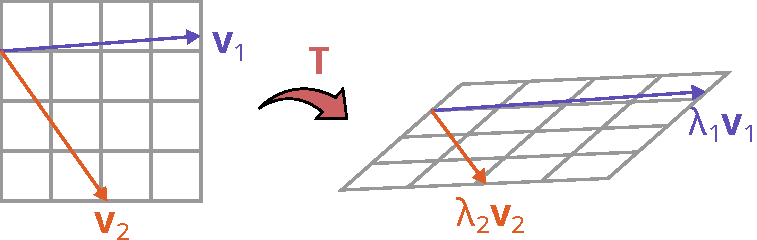
\includegraphics[scale=1]{Figures/10-Consideracoes/Autovalor.pdf}
                \caption{Autovalores e autovetores de uma transformação linear}
                \label{fig:autovalor}
            \end{figure}

            Matrizes de rigidez em elementos finitos (após aplicação das condições de contorno) são positivo definidas, isto é:

            \begin{equation}
                \lambda_i > 0
            \end{equation}

            Um vetor qualquer no espaço $n$ dimensional pode ser escrito como uma combinação linear dos autovetores. Por exemplo, para $n = 2$:

            \begin{equation}
                \bm{u} = a_1 \bm{v}_1 + a_2 \bm{v}_2
            \end{equation}

            \begin{equation}
                \bm{K}\bm{u} 
                = a_1 \lambda_1 \bm{v}_1 + a_2 \lambda_2 \bm{v}_2 
                = \lambda_1 \left( a_1 \bm{v}_1 + a_2 \frac{\lambda_2}{\lambda_1} \bm{v}_2\right)
            \end{equation}

            Entretanto, se $\lambda_1 \gg \lambda_2$, assim como no exemplo da mola, podemos perder informações na resposta, visto que $\frac{\lambda_2}{\lambda_1} \approx 0$:

            \begin{equation}
                \bm{K}\bm{u} 
                \approx a_1 \lambda_1 \bm{v}_1
            \end{equation}

            Portanto, se o autovetor associados aos autovalores pequenos tiverem uma contribuição significativa na composição de $\bm{u}$, podemos perder informações significativas sobre este. Importante salientar que isso indica apenas uma \textbf{possível} perda de precisão na resposta, isso não significa que efetivamente \textbf{teremos} a precisão afetada.

            Para medir a possível perda de precisão na resposta, define-se o número de condicionamento:

            \begin{equation}
                C(\bm{K}) = \frac{\lambda_\text{max}}{\lambda_\text{min}}
            \end{equation}

            \noindent no qual $\lambda_\text{max}$ e $\lambda_\text{min}$ são, respectivamente, o maior e o menor autovalor da matriz $\bm{K}$.

            Um número de condicionamento elevado está, usualmente associado a perda de informação no autovetor associado ao menor autovalor. Na prática, pode-se utilizar a seguinte expressão:

            \begin{equation}
                \text{perda de precisão} \approx \text{log}_{10} C(\bm{K}) = \text{log}_{10} \frac{\lambda_\text{max}}{\lambda_\text{min}}
            \end{equation}

            \noindent no qual a perda de precisão é o número de casas decimais (a partir da menor) nos quais há erros numéricos.

    \subsection{Refino p e h}

    \subsection{Singularidades}


	
	
 
	\cleardoublepage
	\section*{Apêndice}%
    \addcontentsline{toc}{section}{Apêndice}%
    \markright{Apêndice}
	\setcounter{subsection}{0}
	\renewcommand\thesubsection{\Alph{subsection}}
	
	%LTeX: language=pt-br
% !TeX root = Apostila_IM381.tex

\subsection{Superconvergência}
\label{app:superconvergencia}

    Para o problema de barra, o deslocamento nodal será igual ao deslocamento analítico. Neste apêndice, vamos provar isso.

    Sem perda de generalidade, considere a equação diferencial da barra na forma:

    \begin{equation}
        \begin{array}{l}
            u''(x) + p(x) = 0\\
            u(0) = u_0\\
            u'(1) = F
        \end{array}
        \label{eq:fraca_apendice}
    \end{equation}

    \noindent no qual esta equação assume $EA=1$ e $L=1$. Estas hipóteses simplificam a dedução, sem alterar a conclusão.

    Antes de prosseguir, precisamos definir o conceito de função de Green. A função de Green ($g(x)$) correspondente à equação acima, é a função que resolve o problema com uma única força concentrada em um ponto $y$, ou seja, a força é representada por uma função delta de Dirac $\delta_y = \left\langle x-y\right\rangle^{-1}$:


    \begin{equation}
        \begin{array}{l}
            g''(x) + \delta_y = 0\\
            g(0) = 0\\
            g'(1) = 0
        \end{array}
    \end{equation}

    Este problema pode ser resolvido utilizando as funções de singularidade da Seção \ref{sec:singularidade}. A solução então fica:

    \begin{equation*}
        g(x) = -\left\langle x-y\right\rangle^1 + C_1x + C_2
    \end{equation*}

    Aplicando as condições de contorno:

    \begin{equation*}
        g(x) = x-\left\langle x-y\right\rangle^1
    \end{equation*}

    A função de Green obtida é a expressão de duas retas, que ligam, respectivamente, pontos com coordenadas $x=0$, $x=y$ e $x=1$.

    Considere agora a forma fraca do problema com a função de Green:

    \begin{equation*}
        a(w,g) = (w,\delta_y)
    \end{equation*}

    \begin{equation*}
        \int_{0}^{1} w'(x)g'(x) dx + \int_{0}^{1} w(x)\left\langle x-y\right\rangle^{-1} dx = 0 \quad, \forall w(x) \in W
    \end{equation*}

    \begin{equation*}
        \int_{0}^{1} w'(x)g'(x) dx + w(y) = 0 \quad, \forall w(x) \in W
        \label{eq:green}
    \end{equation*}

    Para provar a superconvergência, precisaremos de duas relações. A primeira é:

    \begin{equation}
        a(w^h, u-u^h)=0
        \label{eq:lem1}
    \end{equation}

    Para provar essa relação, partimos da forma fraca da aproximação de Eq. \eqref{eq:fraca_apendice} e da sua forma fraca com os mesmos $w^h(x)$:

    \begin{equation*}
        a(w^h, u) = (w^h, p) + w^h(L)F
    \end{equation*}

    \begin{equation*}
        a(w^h, u^h) = (w^h, p) + w^h(L)F
    \end{equation*}

    Subtraindo as duas expressões 

    \begin{equation*}
        a(w^h, u) - a(w^h, u^h) = 0
    \end{equation*}

    \begin{equation*}
        a(w^h, u-u^h) = 0
    \end{equation*}

    A segunda relação é:

    \begin{equation}
        u(y) - u^h(y) = a(u-u^h, g)
        \label{eq:lem2}
    \end{equation}

    Para provar, partimos da definição do delta de Dirac:

    \begin{equation}
        (u,\delta_y) = \int_{0}^{1} u(x) \delta_y = u(y)
    \end{equation}

    Portanto,

    \begin{equation}
        (u-u^h,\delta_y) = u(y) - u^h(y)
    \end{equation}

    Da Eq. \eqref{eq:green}:

    \begin{equation}
        (u-u^h,\delta_y) = a(u-u^h,g)
    \end{equation}

    Portanto,

    \begin{equation}
        u(y) - u^h(y) = a(u-u^h,g)
    \end{equation}

    Juntaremos agora a Eq. \eqref{eq:lem1} com a Eq. \eqref{eq:lem2}. Além disso, sabemos que a função de Green $g(x)$ representa retas que ligam pontos. Se $x=y$ for um nó da malha, então as funções de forma lineares de $w^h(x)$ conseguem representar de forma exata $g(x)$, isto é $g(x) \in W^h$.

    \begin{equation*}
        u(y) - u^h(y) = a(u-u^h,g) = a(g, u-u^h) = 0
    \end{equation*}

    \begin{equation}
        u(y) = u^h(y)
    \end{equation}

    Desta forma, fica provado que, para o elemento de barra, a solução aproximada $u^h(y)$ será exata para os pontos $x=y$ que são coordenadas de algum nó da malha.


\end{document}
